%%%%%%%%%%%%%%%%%%%%%%%%%%%%%%%%%%%%%%%%%%%%%%%%%%%%%%%%%%%%%%%%%%%%%%%%
%%% P1 --- AAMAS 2027 main track submission
%%%
%%% Working title: What Is This Memory Useful For?
%%%
%%% STATUS: SKELETON. Contains NO results. Every number in this paper must
%%% appear in docs/RESULTS_LEDGER.md in the code repository FIRST, with the
%%% artifact path that produced it and the date it was measured.
%%%
%%% HARD CONSTRAINTS (verified from the AAMAS 2027 site on 2026-09-29):
%%%   * at most EIGHT pages, references unlimited
%%%   * an appendix in the main paper COUNTS toward the 8 pages
%%%     (this differs from AAMAS 2026) --- put overflow in supplementary
%%%   * double-blind; do not de-anonymize, including supplementary
%%%   * do not modify aamas.cls or any layout parameter
%%%   * AI-assistance disclosure is REQUIRED where AI shaped hypotheses or
%%%     experimental design: prompt + tool + version
%%%   * hallucinated citations are a named desk-reject trigger ---
%%%     every \cite must be human-verified against a fetched source
%%%%%%%%%%%%%%%%%%%%%%%%%%%%%%%%%%%%%%%%%%%%%%%%%%%%%%%%%%%%%%%%%%%%%%%%

\documentclass[sigconf,anonymous]{aamas}

\usepackage{balance}
\usepackage{booktabs}
\usepackage{amsmath}
%%% Figures are drawn in TikZ INSIDE this document: no external assets, no
%%% downloaded packages, reproducible from source alone. Data-bearing figures
%%% are generated by scripts/make_figures.py in the code repository, which
%%% emits the coordinate macros below from the tracked artifacts -- no number
%%% in any figure is hand-typed.
\usepackage{tikz}
\usetikzlibrary{positioning,calc,fit,arrows.meta,backgrounds}
%%% Generated figure data: every number inside a data-bearing figure, recomputed
%%% from the tracked artifacts. Regenerate with `python3 scripts/make_figures.py`
%%% in the code repository. Do not edit figdata.tex by hand.
%%% (No absolute path here on purpose: LaTeX source is often uploaded with the
%%% submission, and a home directory in a comment de-anonymizes it.)
%%% GENERATED by scripts/make_figures.py in the code repository.
%%% DO NOT EDIT BY HAND, and do not edit a value here to make a
%%% figure look right -- regenerate. Every value is recomputed from
%%% a tracked artifact and cross-checked against the audited value;
%%% the generator exits non-zero on any disagreement, and a planted
%%% sign flip in one BEARING cell is verified to make it fail.
%%% Sources: data/manifests/lmev2_leakage_small.jsonl
%%%          results/ledgers/repro/screened_cells_slim.jsonl
%%%          results/ledgers/k1_screened_design.json (basis pin)

%% --- sparsity map (fig 1b): one square per MEASURED cell ---
%% The paper's central claim, drawn at cell level. dU is exactly
%% three-valued (-1/0/+1) and the generator FAILS if a fourth
%% level appears. Unmeasured slots are drawn as NOTHING: the
%% rows are ragged, and padding them to a rectangle collapses
%% the BEARING/RANDOM contrast from 3.83x to 1.02x -- both
%% readings are asserted so a padded redraw cannot pass.
\def\spPos{0.00/0.00,4.20/0.00,8.40/0.00,46.80/0.00,93.60/0.00,0.00/-2.55,4.20/-2.55,8.40/-2.55,46.80/-2.55,93.60/-2.55,0.00/-5.10,4.20/-5.10,8.40/-5.10,46.80/-5.10,93.60/-5.10,97.80/-5.10,0.00/-7.65,4.20/-7.65,8.40/-7.65,93.60/-7.65,97.80/-7.65,0.00/-10.20,4.20/-10.20,46.80/-10.20,51.00/-10.20,0.00/-12.75,4.20/-12.75,93.60/-12.75,0.00/-15.30,4.20/-15.30,93.60/-15.30,97.80/-15.30,0.00/-17.85,4.20/-17.85,0.00/-20.40,4.20/-20.40,0.00/-22.95,4.20/-22.95,93.60/-22.95,0.00/-25.50,4.20/-25.50,93.60/-25.50,97.80/-25.50,102.00/-25.50,0.00/-28.05,4.20/-28.05,93.60/-28.05,97.80/-28.05,102.00/-28.05,0.00/-30.60,4.20/-30.60,93.60/-30.60,97.80/-30.60,0.00/-33.15,4.20/-33.15,93.60/-33.15,0.00/-35.70,46.80/-35.70,93.60/-35.70,0.00/-38.25,0.00/-40.80,93.60/-40.80,0.00/-43.35,0.00/-45.90,93.60/-45.90,97.80/-45.90,0.00/-48.45,93.60/-48.45,97.80/-48.45,0.00/-51.00,93.60/-51.00,0.00/-53.55,93.60/-53.55,0.00/-56.10,93.60/-56.10,97.80/-56.10,102.00/-56.10,0.00/-58.65,93.60/-58.65,0.00/-61.20,93.60/-61.20,97.80/-61.20,0.00/-63.75,46.80/-63.75,93.60/-63.75,0.00/-66.30,0.00/-68.85,93.60/-68.85,0.00/-71.40,93.60/-71.40,97.80/-71.40,0.00/-73.95,0.00/-76.50,46.80/-76.50,93.60/-76.50,97.80/-76.50,102.00/-76.50,106.20/-76.50,0.00/-79.05,93.60/-79.05,97.80/-79.05,93.60/-81.60,93.60/-84.15,97.80/-84.15,93.60/-86.70,93.60/-89.25,97.80/-89.25,93.60/-94.35,97.80/-94.35,46.80/-96.90,93.60/-96.90,97.80/-96.90,102.00/-96.90,93.60/-99.45,93.60/-102.00,93.60/-104.55,97.80/-104.55,93.60/-107.10,93.60/-109.65,97.80/-109.65,93.60/-112.20,93.60/-114.75,93.60/-117.30,97.80/-117.30,93.60/-119.85,93.60/-122.40,93.60/-124.95,93.60/-127.50,93.60/-130.05,97.80/-130.05,102.00/-130.05,46.80/-132.60,93.60/-135.15,93.60/-137.70,93.60/-140.25,97.80/-140.25,93.60/-142.80,93.60/-145.35,93.60/-147.90,93.60/-150.45,97.80/-150.45,102.00/-150.45}
\def\spNeg{59.40/-7.65,152.40/-7.65,80.40/-10.20,139.80/-10.20,67.80/-15.30,148.20/-15.30,152.40/-17.85,148.20/-28.05,148.20/-38.25,152.40/-38.25,144.00/-45.90,148.20/-45.90,152.40/-45.90,152.40/-48.45,148.20/-51.00,46.80/-53.55,144.00/-61.20,148.20/-61.20,148.20/-66.30,152.40/-66.30,152.40/-71.40,152.40/-79.05,12.60/-81.60,55.20/-84.15,55.20/-86.70,4.20/-99.45,152.40/-114.75,148.20/-117.30,152.40/-122.40,152.40/-124.95,152.40/-130.05,152.40/-137.70,152.40/-142.80,152.40/-150.45}
\def\spZero{12.60/0.00,16.80/0.00,21.00/0.00,25.20/0.00,29.40/0.00,33.60/0.00,51.00/0.00,55.20/0.00,59.40/0.00,63.60/0.00,67.80/0.00,72.00/0.00,76.20/0.00,80.40/0.00,97.80/0.00,102.00/0.00,106.20/0.00,110.40/0.00,114.60/0.00,118.80/0.00,123.00/0.00,127.20/0.00,131.40/0.00,135.60/0.00,139.80/0.00,144.00/0.00,148.20/0.00,12.60/-2.55,16.80/-2.55,21.00/-2.55,25.20/-2.55,29.40/-2.55,51.00/-2.55,55.20/-2.55,59.40/-2.55,63.60/-2.55,67.80/-2.55,72.00/-2.55,76.20/-2.55,80.40/-2.55,97.80/-2.55,102.00/-2.55,106.20/-2.55,110.40/-2.55,114.60/-2.55,118.80/-2.55,123.00/-2.55,127.20/-2.55,131.40/-2.55,135.60/-2.55,139.80/-2.55,12.60/-5.10,51.00/-5.10,55.20/-5.10,59.40/-5.10,102.00/-5.10,106.20/-5.10,110.40/-5.10,114.60/-5.10,118.80/-5.10,123.00/-5.10,127.20/-5.10,131.40/-5.10,135.60/-5.10,139.80/-5.10,144.00/-5.10,148.20/-5.10,152.40/-5.10,46.80/-7.65,51.00/-7.65,55.20/-7.65,102.00/-7.65,106.20/-7.65,110.40/-7.65,114.60/-7.65,118.80/-7.65,123.00/-7.65,127.20/-7.65,131.40/-7.65,135.60/-7.65,139.80/-7.65,144.00/-7.65,148.20/-7.65,8.40/-10.20,12.60/-10.20,16.80/-10.20,21.00/-10.20,25.20/-10.20,29.40/-10.20,55.20/-10.20,59.40/-10.20,63.60/-10.20,67.80/-10.20,72.00/-10.20,76.20/-10.20,93.60/-10.20,97.80/-10.20,102.00/-10.20,106.20/-10.20,110.40/-10.20,114.60/-10.20,118.80/-10.20,123.00/-10.20,127.20/-10.20,131.40/-10.20,135.60/-10.20,8.40/-12.75,12.60/-12.75,16.80/-12.75,46.80/-12.75,51.00/-12.75,55.20/-12.75,59.40/-12.75,63.60/-12.75,67.80/-12.75,97.80/-12.75,102.00/-12.75,106.20/-12.75,110.40/-12.75,114.60/-12.75,118.80/-12.75,123.00/-12.75,127.20/-12.75,131.40/-12.75,135.60/-12.75,139.80/-12.75,144.00/-12.75,148.20/-12.75,8.40/-15.30,12.60/-15.30,16.80/-15.30,46.80/-15.30,51.00/-15.30,55.20/-15.30,59.40/-15.30,63.60/-15.30,102.00/-15.30,106.20/-15.30,110.40/-15.30,114.60/-15.30,118.80/-15.30,123.00/-15.30,127.20/-15.30,131.40/-15.30,135.60/-15.30,139.80/-15.30,144.00/-15.30,8.40/-17.85,46.80/-17.85,51.00/-17.85,55.20/-17.85,59.40/-17.85,93.60/-17.85,97.80/-17.85,102.00/-17.85,106.20/-17.85,110.40/-17.85,114.60/-17.85,118.80/-17.85,123.00/-17.85,127.20/-17.85,131.40/-17.85,135.60/-17.85,139.80/-17.85,144.00/-17.85,148.20/-17.85,8.40/-20.40,46.80/-20.40,51.00/-20.40,55.20/-20.40,93.60/-20.40,97.80/-20.40,102.00/-20.40,106.20/-20.40,110.40/-20.40,114.60/-20.40,118.80/-20.40,123.00/-20.40,127.20/-20.40,131.40/-20.40,135.60/-20.40,139.80/-20.40,144.00/-20.40,148.20/-20.40,152.40/-20.40,8.40/-22.95,46.80/-22.95,51.00/-22.95,55.20/-22.95,97.80/-22.95,102.00/-22.95,106.20/-22.95,110.40/-22.95,114.60/-22.95,118.80/-22.95,123.00/-22.95,127.20/-22.95,131.40/-22.95,135.60/-22.95,139.80/-22.95,144.00/-22.95,148.20/-22.95,152.40/-22.95,8.40/-25.50,46.80/-25.50,51.00/-25.50,55.20/-25.50,106.20/-25.50,110.40/-25.50,114.60/-25.50,118.80/-25.50,123.00/-25.50,127.20/-25.50,131.40/-25.50,135.60/-25.50,139.80/-25.50,144.00/-25.50,148.20/-25.50,8.40/-28.05,46.80/-28.05,51.00/-28.05,55.20/-28.05,106.20/-28.05,110.40/-28.05,114.60/-28.05,118.80/-28.05,123.00/-28.05,127.20/-28.05,131.40/-28.05,135.60/-28.05,139.80/-28.05,144.00/-28.05,46.80/-30.60,51.00/-30.60,102.00/-30.60,106.20/-30.60,110.40/-30.60,114.60/-30.60,118.80/-30.60,123.00/-30.60,127.20/-30.60,131.40/-30.60,135.60/-30.60,139.80/-30.60,144.00/-30.60,148.20/-30.60,152.40/-30.60,46.80/-33.15,51.00/-33.15,97.80/-33.15,102.00/-33.15,106.20/-33.15,110.40/-33.15,114.60/-33.15,118.80/-33.15,123.00/-33.15,127.20/-33.15,131.40/-33.15,135.60/-33.15,139.80/-33.15,144.00/-33.15,148.20/-33.15,4.20/-35.70,8.40/-35.70,12.60/-35.70,51.00/-35.70,55.20/-35.70,59.40/-35.70,97.80/-35.70,102.00/-35.70,106.20/-35.70,110.40/-35.70,114.60/-35.70,118.80/-35.70,123.00/-35.70,127.20/-35.70,131.40/-35.70,135.60/-35.70,139.80/-35.70,144.00/-35.70,4.20/-38.25,8.40/-38.25,46.80/-38.25,51.00/-38.25,55.20/-38.25,59.40/-38.25,93.60/-38.25,97.80/-38.25,102.00/-38.25,106.20/-38.25,110.40/-38.25,114.60/-38.25,118.80/-38.25,123.00/-38.25,127.20/-38.25,131.40/-38.25,135.60/-38.25,139.80/-38.25,144.00/-38.25,4.20/-40.80,46.80/-40.80,51.00/-40.80,97.80/-40.80,102.00/-40.80,106.20/-40.80,110.40/-40.80,114.60/-40.80,118.80/-40.80,123.00/-40.80,127.20/-40.80,131.40/-40.80,135.60/-40.80,139.80/-40.80,144.00/-40.80,148.20/-40.80,4.20/-43.35,46.80/-43.35,51.00/-43.35,93.60/-43.35,97.80/-43.35,102.00/-43.35,106.20/-43.35,110.40/-43.35,114.60/-43.35,118.80/-43.35,123.00/-43.35,127.20/-43.35,131.40/-43.35,135.60/-43.35,139.80/-43.35,144.00/-43.35,148.20/-43.35,4.20/-45.90,46.80/-45.90,51.00/-45.90,102.00/-45.90,106.20/-45.90,110.40/-45.90,114.60/-45.90,118.80/-45.90,123.00/-45.90,127.20/-45.90,131.40/-45.90,135.60/-45.90,139.80/-45.90,4.20/-48.45,46.80/-48.45,51.00/-48.45,102.00/-48.45,106.20/-48.45,110.40/-48.45,114.60/-48.45,118.80/-48.45,123.00/-48.45,127.20/-48.45,131.40/-48.45,135.60/-48.45,139.80/-48.45,144.00/-48.45,148.20/-48.45,4.20/-51.00,46.80/-51.00,51.00/-51.00,97.80/-51.00,102.00/-51.00,106.20/-51.00,110.40/-51.00,114.60/-51.00,118.80/-51.00,123.00/-51.00,127.20/-51.00,131.40/-51.00,135.60/-51.00,139.80/-51.00,144.00/-51.00,97.80/-53.55,102.00/-53.55,106.20/-53.55,110.40/-53.55,114.60/-53.55,118.80/-53.55,123.00/-53.55,127.20/-53.55,131.40/-53.55,135.60/-53.55,139.80/-53.55,144.00/-53.55,148.20/-53.55,152.40/-53.55,46.80/-56.10,106.20/-56.10,110.40/-56.10,114.60/-56.10,118.80/-56.10,123.00/-56.10,127.20/-56.10,131.40/-56.10,135.60/-56.10,139.80/-56.10,144.00/-56.10,148.20/-56.10,152.40/-56.10,46.80/-58.65,97.80/-58.65,102.00/-58.65,106.20/-58.65,110.40/-58.65,114.60/-58.65,118.80/-58.65,123.00/-58.65,127.20/-58.65,131.40/-58.65,135.60/-58.65,139.80/-58.65,144.00/-58.65,148.20/-58.65,152.40/-58.65,46.80/-61.20,102.00/-61.20,106.20/-61.20,110.40/-61.20,114.60/-61.20,118.80/-61.20,123.00/-61.20,127.20/-61.20,131.40/-61.20,135.60/-61.20,139.80/-61.20,97.80/-63.75,102.00/-63.75,106.20/-63.75,110.40/-63.75,114.60/-63.75,118.80/-63.75,123.00/-63.75,127.20/-63.75,131.40/-63.75,135.60/-63.75,139.80/-63.75,144.00/-63.75,148.20/-63.75,46.80/-66.30,93.60/-66.30,97.80/-66.30,102.00/-66.30,106.20/-66.30,110.40/-66.30,114.60/-66.30,118.80/-66.30,123.00/-66.30,127.20/-66.30,131.40/-66.30,135.60/-66.30,139.80/-66.30,144.00/-66.30,46.80/-68.85,97.80/-68.85,102.00/-68.85,106.20/-68.85,110.40/-68.85,114.60/-68.85,118.80/-68.85,123.00/-68.85,127.20/-68.85,131.40/-68.85,135.60/-68.85,139.80/-68.85,144.00/-68.85,148.20/-68.85,152.40/-68.85,46.80/-71.40,102.00/-71.40,106.20/-71.40,110.40/-71.40,114.60/-71.40,118.80/-71.40,123.00/-71.40,127.20/-71.40,131.40/-71.40,135.60/-71.40,139.80/-71.40,144.00/-71.40,148.20/-71.40,46.80/-73.95,93.60/-73.95,97.80/-73.95,102.00/-73.95,106.20/-73.95,110.40/-73.95,114.60/-73.95,118.80/-73.95,123.00/-73.95,127.20/-73.95,131.40/-73.95,135.60/-73.95,139.80/-73.95,144.00/-73.95,148.20/-73.95,110.40/-76.50,114.60/-76.50,118.80/-76.50,123.00/-76.50,127.20/-76.50,131.40/-76.50,135.60/-76.50,139.80/-76.50,144.00/-76.50,148.20/-76.50,152.40/-76.50,46.80/-79.05,102.00/-79.05,106.20/-79.05,110.40/-79.05,114.60/-79.05,118.80/-79.05,123.00/-79.05,127.20/-79.05,131.40/-79.05,135.60/-79.05,139.80/-79.05,144.00/-79.05,148.20/-79.05,0.00/-81.60,4.20/-81.60,8.40/-81.60,46.80/-81.60,51.00/-81.60,55.20/-81.60,59.40/-81.60,97.80/-81.60,102.00/-81.60,106.20/-81.60,110.40/-81.60,114.60/-81.60,118.80/-81.60,123.00/-81.60,127.20/-81.60,131.40/-81.60,135.60/-81.60,139.80/-81.60,144.00/-81.60,148.20/-81.60,152.40/-81.60,0.00/-84.15,4.20/-84.15,8.40/-84.15,46.80/-84.15,51.00/-84.15,102.00/-84.15,106.20/-84.15,110.40/-84.15,114.60/-84.15,118.80/-84.15,123.00/-84.15,127.20/-84.15,131.40/-84.15,135.60/-84.15,139.80/-84.15,144.00/-84.15,148.20/-84.15,0.00/-86.70,4.20/-86.70,8.40/-86.70,46.80/-86.70,51.00/-86.70,97.80/-86.70,102.00/-86.70,106.20/-86.70,110.40/-86.70,114.60/-86.70,118.80/-86.70,123.00/-86.70,127.20/-86.70,131.40/-86.70,135.60/-86.70,139.80/-86.70,144.00/-86.70,148.20/-86.70,152.40/-86.70,0.00/-89.25,4.20/-89.25,8.40/-89.25,46.80/-89.25,51.00/-89.25,55.20/-89.25,102.00/-89.25,106.20/-89.25,110.40/-89.25,114.60/-89.25,118.80/-89.25,123.00/-89.25,127.20/-89.25,131.40/-89.25,135.60/-89.25,139.80/-89.25,144.00/-89.25,148.20/-89.25,0.00/-91.80,4.20/-91.80,8.40/-91.80,46.80/-91.80,51.00/-91.80,55.20/-91.80,93.60/-91.80,97.80/-91.80,102.00/-91.80,106.20/-91.80,110.40/-91.80,114.60/-91.80,118.80/-91.80,123.00/-91.80,127.20/-91.80,131.40/-91.80,135.60/-91.80,139.80/-91.80,144.00/-91.80,148.20/-91.80,152.40/-91.80,0.00/-94.35,4.20/-94.35,8.40/-94.35,46.80/-94.35,51.00/-94.35,55.20/-94.35,102.00/-94.35,106.20/-94.35,110.40/-94.35,114.60/-94.35,118.80/-94.35,123.00/-94.35,127.20/-94.35,131.40/-94.35,135.60/-94.35,139.80/-94.35,144.00/-94.35,148.20/-94.35,152.40/-94.35,0.00/-96.90,4.20/-96.90,8.40/-96.90,51.00/-96.90,55.20/-96.90,106.20/-96.90,110.40/-96.90,114.60/-96.90,118.80/-96.90,123.00/-96.90,127.20/-96.90,131.40/-96.90,135.60/-96.90,139.80/-96.90,144.00/-96.90,148.20/-96.90,0.00/-99.45,46.80/-99.45,51.00/-99.45,97.80/-99.45,102.00/-99.45,106.20/-99.45,110.40/-99.45,114.60/-99.45,118.80/-99.45,123.00/-99.45,127.20/-99.45,131.40/-99.45,135.60/-99.45,139.80/-99.45,144.00/-99.45,0.00/-102.00,4.20/-102.00,46.80/-102.00,51.00/-102.00,97.80/-102.00,102.00/-102.00,106.20/-102.00,110.40/-102.00,114.60/-102.00,118.80/-102.00,123.00/-102.00,127.20/-102.00,131.40/-102.00,135.60/-102.00,139.80/-102.00,144.00/-102.00,148.20/-102.00,152.40/-102.00,0.00/-104.55,4.20/-104.55,46.80/-104.55,51.00/-104.55,102.00/-104.55,106.20/-104.55,110.40/-104.55,114.60/-104.55,118.80/-104.55,123.00/-104.55,127.20/-104.55,131.40/-104.55,135.60/-104.55,139.80/-104.55,144.00/-104.55,148.20/-104.55,0.00/-107.10,4.20/-107.10,46.80/-107.10,51.00/-107.10,97.80/-107.10,102.00/-107.10,106.20/-107.10,110.40/-107.10,114.60/-107.10,118.80/-107.10,123.00/-107.10,127.20/-107.10,131.40/-107.10,135.60/-107.10,139.80/-107.10,144.00/-107.10,148.20/-107.10,0.00/-109.65,4.20/-109.65,46.80/-109.65,51.00/-109.65,102.00/-109.65,106.20/-109.65,110.40/-109.65,114.60/-109.65,118.80/-109.65,123.00/-109.65,127.20/-109.65,131.40/-109.65,135.60/-109.65,139.80/-109.65,144.00/-109.65,148.20/-109.65,152.40/-109.65,0.00/-112.20,4.20/-112.20,46.80/-112.20,51.00/-112.20,97.80/-112.20,102.00/-112.20,106.20/-112.20,110.40/-112.20,114.60/-112.20,118.80/-112.20,123.00/-112.20,127.20/-112.20,131.40/-112.20,135.60/-112.20,139.80/-112.20,144.00/-112.20,148.20/-112.20,152.40/-112.20,0.00/-114.75,4.20/-114.75,46.80/-114.75,51.00/-114.75,97.80/-114.75,102.00/-114.75,106.20/-114.75,110.40/-114.75,114.60/-114.75,118.80/-114.75,123.00/-114.75,127.20/-114.75,131.40/-114.75,135.60/-114.75,139.80/-114.75,144.00/-114.75,148.20/-114.75,0.00/-117.30,46.80/-117.30,102.00/-117.30,106.20/-117.30,110.40/-117.30,114.60/-117.30,118.80/-117.30,123.00/-117.30,127.20/-117.30,131.40/-117.30,135.60/-117.30,139.80/-117.30,144.00/-117.30,0.00/-119.85,46.80/-119.85,97.80/-119.85,102.00/-119.85,106.20/-119.85,110.40/-119.85,114.60/-119.85,118.80/-119.85,123.00/-119.85,127.20/-119.85,131.40/-119.85,135.60/-119.85,139.80/-119.85,144.00/-119.85,148.20/-119.85,152.40/-119.85,0.00/-122.40,46.80/-122.40,97.80/-122.40,102.00/-122.40,106.20/-122.40,110.40/-122.40,114.60/-122.40,118.80/-122.40,123.00/-122.40,127.20/-122.40,131.40/-122.40,135.60/-122.40,139.80/-122.40,144.00/-122.40,148.20/-122.40,0.00/-124.95,46.80/-124.95,97.80/-124.95,102.00/-124.95,106.20/-124.95,110.40/-124.95,114.60/-124.95,118.80/-124.95,123.00/-124.95,127.20/-124.95,131.40/-124.95,135.60/-124.95,139.80/-124.95,144.00/-124.95,148.20/-124.95,0.00/-127.50,46.80/-127.50,97.80/-127.50,102.00/-127.50,106.20/-127.50,110.40/-127.50,114.60/-127.50,118.80/-127.50,123.00/-127.50,127.20/-127.50,131.40/-127.50,135.60/-127.50,139.80/-127.50,144.00/-127.50,148.20/-127.50,152.40/-127.50,0.00/-130.05,46.80/-130.05,106.20/-130.05,110.40/-130.05,114.60/-130.05,118.80/-130.05,123.00/-130.05,127.20/-130.05,131.40/-130.05,135.60/-130.05,139.80/-130.05,144.00/-130.05,148.20/-130.05,0.00/-132.60,93.60/-132.60,97.80/-132.60,102.00/-132.60,106.20/-132.60,110.40/-132.60,114.60/-132.60,118.80/-132.60,123.00/-132.60,127.20/-132.60,131.40/-132.60,135.60/-132.60,139.80/-132.60,144.00/-132.60,148.20/-132.60,152.40/-132.60,0.00/-135.15,46.80/-135.15,97.80/-135.15,102.00/-135.15,106.20/-135.15,110.40/-135.15,114.60/-135.15,118.80/-135.15,123.00/-135.15,127.20/-135.15,131.40/-135.15,135.60/-135.15,139.80/-135.15,144.00/-135.15,148.20/-135.15,152.40/-135.15,0.00/-137.70,46.80/-137.70,97.80/-137.70,102.00/-137.70,106.20/-137.70,110.40/-137.70,114.60/-137.70,118.80/-137.70,123.00/-137.70,127.20/-137.70,131.40/-137.70,135.60/-137.70,139.80/-137.70,144.00/-137.70,148.20/-137.70,0.00/-140.25,46.80/-140.25,102.00/-140.25,106.20/-140.25,110.40/-140.25,114.60/-140.25,118.80/-140.25,123.00/-140.25,127.20/-140.25,131.40/-140.25,135.60/-140.25,139.80/-140.25,144.00/-140.25,148.20/-140.25,152.40/-140.25,0.00/-142.80,46.80/-142.80,97.80/-142.80,102.00/-142.80,106.20/-142.80,110.40/-142.80,114.60/-142.80,118.80/-142.80,123.00/-142.80,127.20/-142.80,131.40/-142.80,135.60/-142.80,139.80/-142.80,144.00/-142.80,148.20/-142.80,0.00/-145.35,46.80/-145.35,97.80/-145.35,102.00/-145.35,106.20/-145.35,110.40/-145.35,114.60/-145.35,118.80/-145.35,123.00/-145.35,127.20/-145.35,131.40/-145.35,135.60/-145.35,139.80/-145.35,144.00/-145.35,148.20/-145.35,152.40/-145.35,0.00/-147.90,46.80/-147.90,97.80/-147.90,102.00/-147.90,106.20/-147.90,110.40/-147.90,114.60/-147.90,118.80/-147.90,123.00/-147.90,127.20/-147.90,131.40/-147.90,135.60/-147.90,139.80/-147.90,144.00/-147.90,148.20/-147.90,152.40/-147.90,0.00/-150.45,46.80/-150.45,106.20/-150.45,110.40/-150.45,114.60/-150.45,118.80/-150.45,123.00/-150.45,127.20/-150.45,131.40/-150.45,135.60/-150.45,139.80/-150.45,144.00/-150.45,148.20/-150.45}
\def\spCW{4.20pt}
\def\spRH{2.55pt}
\def\spTotW{156.60pt}
\def\spTotH{153.00pt}
\def\spBearX{0.00pt}
\def\spBearW{37.80pt}
\def\spBearMid{18.90pt}
\def\spBearN{139}
\def\spBearPos{50}
\def\spBearNeg{2}
\def\spBearRate{36.0}
\def\spBearLo{28.5}
\def\spBearHi{44.2}
\def\spCtrlX{46.80pt}
\def\spCtrlW{37.80pt}
\def\spCtrlMid{65.70pt}
\def\spCtrlN{146}
\def\spCtrlPos{10}
\def\spCtrlNeg{6}
\def\spCtrlRate{6.8}
\def\spCtrlLo{3.8}
\def\spCtrlHi{12.1}
\def\spRandX{93.60pt}
\def\spRandW{63.00pt}
\def\spRandMid{125.10pt}
\def\spRandN{872}
\def\spRandPos{82}
\def\spRandNeg{26}
\def\spRandRate{9.4}
\def\spRandLo{7.6}
\def\spRandHi{11.5}
\def\spCells{1{,}157}
\def\spMems{60}
\def\spNonzero{176}
\def\spZeroPct{84.8}
\def\spDrawnRatio{3.8}
\def\spBearTasks{56}
\def\spBearHelps{32}
\def\spCtrlTasks{100}
\def\spCtrlHelps{9}
\def\spRandTasks{147}
\def\spRandHelps{51}

%% --- bearing breadth: counts, and log-scaled bar heights in pt ---
\def\bearNZero{1724}
\def\bearHZero{33.00pt}
\def\bearNOne{119}
\def\bearHOne{21.20pt}
\def\bearNTwo{18}
\def\bearHTwo{13.04pt}
\def\bearNThree{18}
\def\bearHThree{13.04pt}
\def\bearNFour{4}
\def\bearHFour{7.13pt}
\def\bearNFive{2}
\def\bearHFive{4.86pt}
\def\bearNSix{1}
\def\bearHSix{3.07pt}
\def\bearNSeven{0}
\def\bearHSeven{0.00pt}
\def\bearNEight{2}
\def\bearHEight{4.86pt}
\def\bearNNine{1}
\def\bearHNine{3.07pt}
\def\bearUnits{1{,}889}
\def\bearAny{165}
\def\bearGeTwo{46}
\def\bearEpisodes{23}
\def\bearDetTasks{75}
\def\bearTickZero{3.07pt}
\def\bearTickOne{10.62pt}
\def\bearTickTwo{20.43pt}
\def\bearTickThree{30.59pt}

%% --- sign reversal: rate and Wilson bounds, as x-offsets in pt ---
\def\flipBearN{35}
\def\flipBearK{0}
\def\flipBearRate{0.0000}
\def\flipBearX{0.00pt}
\def\flipBearXLo{0.00pt}
\def\flipBearXHi{21.10pt}
\def\flipCtrlN{35}
\def\flipCtrlK{1}
\def\flipCtrlRate{0.0286}
\def\flipCtrlX{6.10pt}
\def\flipCtrlXLo{1.08pt}
\def\flipCtrlXHi{31.00pt}
\def\flipRandN{60}
\def\flipRandK{17}
\def\flipRandRate{0.2833}
\def\flipRandX{60.44pt}
\def\flipRandXLo{39.48pt}
\def\flipRandXHi{86.97pt}
\def\flipTickZero{0.00pt}
\def\flipTickOne{21.33pt}
\def\flipTickTwo{42.67pt}
\def\flipTickThree{64.00pt}
\def\flipTickFour{85.33pt}
\def\flipAxisW{96.00pt}
\def\bearAxisW{104.00pt}

%% --- similarity sextiles: y-offsets in pt, DU_MAX = 0.40 ---
\def\simPooledYZero{6.20pt}
\def\simPooledVZero{0.0885}
\def\simRandYZero{6.83pt}
\def\simRandVZero{0.0976}
\def\simXZero{8.33pt}
\def\simPooledYOne{1.09pt}
\def\simPooledVOne{0.0155}
\def\simRandYOne{0.91pt}
\def\simRandVOne{0.0130}
\def\simXOne{25.00pt}
\def\simPooledYTwo{5.80pt}
\def\simPooledVTwo{0.0829}
\def\simRandYTwo{3.78pt}
\def\simRandVTwo{0.0541}
\def\simXTwo{41.67pt}
\def\simPooledYThree{7.62pt}
\def\simPooledVThree{0.1088}
\def\simRandYThree{5.38pt}
\def\simRandVThree{0.0769}
\def\simXThree{58.33pt}
\def\simPooledYFour{7.62pt}
\def\simPooledVFour{0.1088}
\def\simRandYFour{4.26pt}
\def\simRandVFour{0.0608}
\def\simXFour{75.00pt}
\def\simPooledYFive{10.88pt}
\def\simPooledVFive{0.1554}
\def\simRandYFive{6.02pt}
\def\simRandVFive{0.0859}
\def\simXFive{91.67pt}
\def\stratBearY{24.17pt}
\def\stratBearV{+0.3453}
\def\stratBearN{139}
\def\stratCtrlY{1.92pt}
\def\stratCtrlV{+0.0274}
\def\stratCtrlN{146}
\def\stratRandY{4.50pt}
\def\stratRandV{+0.0642}
\def\stratRandN{872}
\def\simTickZero{0.00pt}
\def\simTickOne{7.00pt}
\def\simTickTwo{14.00pt}
\def\simTickThree{21.00pt}
\def\simTickFour{28.00pt}
\def\simAxisW{100.00pt}
\def\simRhoAll{+0.087}
\def\simRhoRand{+0.006}
\def\simCells{1{,}157}
\def\simLoEdge{0.56}
\def\simHiEdge{0.83}

%% --- frontier (fig 4): ONE basis, 277 cells / 57 memories ---
%% x = log10(tokens per cell), y = paired BEARING-control dU.
%% Efficiency is the slope from the origin; it is not a separate
%% number and so cannot disagree with the plotted point.
\def\frRawDU{+0.3174}
\def\frRawLo{+0.192}
\def\frRawHi{+0.448}
\def\frRawY{28.09pt}
\def\frRawYLo{21.25pt}
\def\frRawYHi{35.17pt}
\def\frRawXExp{82.35pt}
\def\frRawXChg{82.35pt}
\def\frRawTokExp{9{,}228}
\def\frRawTokChg{9{,}228}
\def\frRawEffExp{+0.034}
\def\frRawEffChg{+0.034}
\def\frRawNZ{33}
\def\frSumDU{+0.0613}
\def\frSumLo{-0.042}
\def\frSumHi{+0.164}
\def\frSumY{14.19pt}
\def\frSumYLo{8.58pt}
\def\frSumYHi{19.74pt}
\def\frSumXExp{21.33pt}
\def\frSumXChg{54.15pt}
\def\frSumTokExp{323}
\def\frSumTokChg{1{,}960}
\def\frSumEffExp{+0.190}
\def\frSumEffChg{+0.031}
\def\frSumNZ{26}
\def\frStrDU{-0.0498}
\def\frStrLo{-0.143}
\def\frStrHi{+0.038}
\def\frStrY{8.15pt}
\def\frStrYLo{3.07pt}
\def\frStrYHi{12.94pt}
\def\frStrXExp{15.77pt}
\def\frStrXChg{53.71pt}
\def\frStrTokExp{238}
\def\frStrTokChg{1{,}913}
\def\frStrEffExp{-0.209}
\def\frStrEffChg{-0.026}
\def\frStrNZ{20}
\def\frXTickTwo{0.00pt}
\def\frXTickThree{41.90pt}
\def\frXTickFour{83.81pt}
\def\frYTickMinusTwo{0.00pt}
\def\frYTickZero{10.86pt}
\def\frYTickTwo{21.71pt}
\def\frYTickFour{32.57pt}
\def\frZeroY{10.86pt}
\def\frW{88.00pt}
\def\frH{38.00pt}
\def\frCells{277}
\def\frMems{57}
\def\frReuse{4.86}
\def\frRatioExp{5.5}
\def\frRatioChg{1.10}
\def\frFormSum{1{,}637}
\def\frFormStr{1{,}676}

\def\xbSRLmM{-0.1408}
\def\xbSRLmLo{-0.2211}
\def\xbSRLmHi{-0.0601}
\def\xbSRLmN{277}
\def\xbSRScM{+0.0246}
\def\xbSRScLo{-0.0342}
\def\xbSRScHi{+0.0991}
\def\xbSRScN{122}
\def\xbSRSwM{-0.1000}
\def\xbSRSwLo{-0.2250}
\def\xbSRSwHi{+0.0000}
\def\xbSRSwN{40}
\def\xbTRLmM{-0.1625}
\def\xbTRLmLo{-0.2454}
\def\xbTRLmHi{-0.0798}
\def\xbTRLmN{277}
\def\xbTRScM{+0.0328}
\def\xbTRScLo{-0.0342}
\def\xbTRScHi{+0.1200}
\def\xbTRScN{122}
\def\xbTRSwM{-0.0500}
\def\xbTRSwLo{-0.1750}
\def\xbTRSwHi{+0.0750}
\def\xbTRSwN{40}
\def\xbSRLmXM{-20.02pt}
\def\xbSRLmXLo{-31.44pt}
\def\xbSRLmXHi{-8.55pt}
\def\xbSRScXM{3.50pt}
\def\xbSRScXLo{-4.86pt}
\def\xbSRScXHi{14.09pt}
\def\xbSRSwXM{-14.22pt}
\def\xbSRSwXLo{-32.00pt}
\def\xbSRSwXHi{0.00pt}
\def\xbTRLmXM{-23.10pt}
\def\xbTRLmXLo{-34.90pt}
\def\xbTRLmXHi{-11.36pt}
\def\xbTRScXM{4.66pt}
\def\xbTRScXLo{-4.86pt}
\def\xbTRScXHi{17.07pt}
\def\xbTRSwXM{-7.11pt}
\def\xbTRSwXLo{-24.89pt}
\def\xbTRSwXHi{10.67pt}
\def\sciPairs{154}
\def\sciMems{34}
\def\sciTasks{40}
\def\sciArmRuns{924}
\def\sciMatched{122}
\def\sciDiag{0.0}
\def\sciMedTasks{4}
\def\sweMatched{40}
\def\sweLocMiss{38}
\def\sweBafRaw{13/40}
\def\sweRepos{2}
\def\sweDomRepoPct{92}
\def\rgSmDiff{+0.0982}
\def\rgSmLo{+0.0247}
\def\rgSmHi{+0.1730}
\def\rgSmN{550}
\def\rgSmCells{275}
\def\rgSmTasks{123}
\def\rgSmWithout{-0.0364}
\def\rgSmWith{+0.0618}
\def\gfWithoutPct{15.6}
\def\gfWithPct{50.0}
\def\gfN{64}
\def\gfCtlWithoutPct{14.3}
\def\gfCtlWithPct{11.9}
\def\gfCtlN{84}
\def\gfDiff{+0.3676}
\def\gfCells{32}
\def\gfLexBaf{0.744}
\def\gfLlmBaf{0.310}
\def\rgSmWithoutShare{59}
\def\rgSmOss{+0.2182}
\def\rgSmGem{+0.3164}
\def\xbFloorLm{0.025}
\def\xbFloorLmK{7}
\def\xbFloorLmN{285}
\def\xbFloorSc{0.037}
\def\xbFloorScK{5}
\def\xbFloorScN{135}
\def\xbAxisW{64.0pt}
\def\xbAxisMax{0.45}

%% --- reader generalization (fig 6): gpt-oss vs Gemma readers ---
%% Matched cells only: interpretable under BOTH readers at the
%% same replicate depth. Memory text is byte-identical across
%% the two runs (1694/1694 verified), so only the reader differs.
\def\rgRawN{276}
\def\rgRawTasks{124}
\def\rgRawOss{+0.1884}
\def\rgRawGem{+0.3152}
\def\rgRawDiff{+0.1268}
\def\rgRawLo{+0.0496}
\def\rgRawHi{+0.2050}
\def\rgRawXOss{37.49pt}
\def\rgRawXGem{53.98pt}
\def\rgRawXLo{19.45pt}
\def\rgRawXHi{39.64pt}
\def\rgRawXDiff{29.49pt}
\def\rgRawXCiLo{43.94pt}
\def\rgRawXCiHi{64.14pt}
\def\rgRawExcl{yes}
\def\rgRawRAll{+0.520}
\def\rgRawRNz{+0.213}
\def\rgRawNNz{109}
\def\rgRawZeroBoth{167}
\def\rgRawSignK{49}
\def\rgRawSignN{50}
\def\rgRawLabK{216}
\def\rgRawLabN{276}
\def\rgSumN{274}
\def\rgSumTasks{124}
\def\rgSumOss{+0.0511}
\def\rgSumGem{+0.0547}
\def\rgSumDiff{+0.0036}
\def\rgSumLo{-0.0484}
\def\rgSumHi{+0.0612}
\def\rgSumXOss{19.64pt}
\def\rgSumXGem{20.12pt}
\def\rgSumXLo{6.70pt}
\def\rgSumXHi{20.96pt}
\def\rgSumXDiff{13.47pt}
\def\rgSumXCiLo{13.34pt}
\def\rgSumXCiHi{27.60pt}
\def\rgSumExcl{no}
\def\rgSumRAll{+0.370}
\def\rgSumRNz{+0.187}
\def\rgSumNNz{36}
\def\rgSumZeroBoth{238}
\def\rgSumSignK{10}
\def\rgSumSignN{11}
\def\rgSumLabK{248}
\def\rgSumLabN{274}
\def\rgStrN{269}
\def\rgStrTasks{122}
\def\rgStrOss{+0.0186}
\def\rgStrGem{+0.0297}
\def\rgStrDiff{+0.0112}
\def\rgStrLo{-0.0536}
\def\rgStrHi{+0.0833}
\def\rgStrXOss{15.42pt}
\def\rgStrXGem{16.87pt}
\def\rgStrXLo{6.04pt}
\def\rgStrXHi{23.83pt}
\def\rgStrXDiff{14.45pt}
\def\rgStrXCiLo{8.45pt}
\def\rgStrXCiHi{26.25pt}
\def\rgStrExcl{no}
\def\rgStrRAll{-0.008}
\def\rgStrRNz{-0.070}
\def\rgStrNNz{35}
\def\rgStrZeroBoth{234}
\def\rgStrSignK{2}
\def\rgStrSignN{4}
\def\rgStrLabK{236}
\def\rgStrLabN{269}
\def\rgTickZero{13.00pt}
\def\rgTickTwo{39.00pt}
\def\rgTickFour{65.00pt}
\def\rgTickSix{91.00pt}
\def\rgZeroX{13.00pt}
\def\rgW{104.00pt}
\def\rgH{36.00pt}
\def\rgRows{1{,}694}
\def\rgBmcRawOss{+0.3462}
\def\rgBmcRawOssLo{+0.2210}
\def\rgBmcRawOssHi{+0.4761}
\def\rgBmcRawOssMem{59}
\def\rgBmcRawGem{+0.6002}
\def\rgBmcRawGemLo{+0.4787}
\def\rgBmcRawGemHi{+0.7144}
\def\rgBmcRawGemMem{59}
\def\rgWithoutShare{54}
\def\rgWithDelta{+0.0580}
\def\rgWithoutDelta{-0.0688}

%% --- reader transfer, SESSION-MATCHED (fig 6a) ------------
%% CANONICAL. 275 cells / 123 tasks / 550 replicate rows, both
%% arms in ONE session. The superseded cross-session +0.1268 is
%% NOT drawn. Exactly ONE interval is drawn, the PAIRED one:
%% the two readers' marginal intervals overlap by 0.0689, so
%% drawing them would invite a false 'no difference' reading.
\def\smXOss{50.18pt}
\def\smXGem{72.76pt}
\def\smXCiLo{55.86pt}
\def\smXCiHi{89.97pt}
\def\smTickZero{0.00pt}
\def\smTickOne{23.00pt}
\def\smTickTwo{46.00pt}
\def\smTickThree{69.00pt}
\def\smTickFour{92.00pt}
\def\smW{92.00pt}
\def\smCPosPos{55}
\def\smCPosZero{10}
\def\smCPosNeg{1}
\def\smCZeroPos{32}
\def\smCZeroZero{170}
\def\smCZeroNeg{1}
\def\smCNegPos{2}
\def\smCNegZero{4}
\def\smCNegNeg{0}
\def\smAgree{55}
\def\smBoth{58}
\def\smZeroBoth{170}
\def\smIdentN{570}
\def\smIdentK{570}

%% --- coverage (tab 2): eligible / attempted / completed ---
\def\covLmElig{1{,}157}
\def\covLmAtt{1{,}157}
\def\covLmDone{1{,}157}
\def\covLmExcl{0}
\def\covLmPct{100.0}
\def\covScElig{462}
\def\covScAtt{462}
\def\covScDone{391}
\def\covScExcl{71}
\def\covScPct{84.6}
\def\covSwElig{321}
\def\covSwAtt{321}
\def\covSwDone{141}
\def\covSwExcl{180}
\def\covSwPct{43.9}
\def\covScMatched{122}
\def\covSwMatched{40}
\def\covSwRepos{2}
\def\covSwLocMiss{116}
\def\covSwUnscored{62}
\def\covSwUnavail{2}



%%% AAMAS-2027 copyright block (do not change!)
\makeatletter
\gdef\@copyrightpermission{
  \begin{minipage}{0.2\columnwidth}
   \href{https://creativecommons.org/licenses/by/4.0/}{
\includegraphics[width=0.90\textwidth]{by}}
  \end{minipage}\hfill
  \begin{minipage}{0.8\columnwidth}
   \href{https://creativecommons.org/licenses/by/4.0/}{This work is licensed under a Creative Commons Attribution International 4.0 License.}
  \end{minipage}
  \vspace{5pt}
}
\makeatother

\setcopyright{ifaamas}
\acmConference[AAMAS 2027]{Proc.\@ of the 26th International Conference
on Autonomous Agents and Multiagent Systems (AAMAS 2027)}{3--7 May 2027}{Hanoi, Vietnam}{M.~Baldoni, F.~Fang, W.~Yeoh, N.~Yorke-Smith (eds.)}
\copyrightyear{2027}
\acmYear{2027}
\acmDOI{}
\acmISBN{}

%%% TODO: fill in after the abstract is registered on OpenReview.
\acmSubmissionID{<<OpenReview submission id>>}

\title{What Is This Memory Useful For? Measuring Task-Conditioned
Utility in Long-Term Agent Memory}

%%% Anonymous mode suppresses these, but they must be present.
\author{Anonymous Author(s)}
\affiliation{%
  \institution{Anonymous Institution}
  \city{}
  \country{}
}

\begin{document}

\begin{abstract}
%%% Canonical copy: docs/submission/abstract_v5.txt in the code repo.
%%% v6 (2026-10-01, SA-SCI-PAPER) adds the reader-generalization clause and
%%% makes the cross-benchmark BOUNDARY explicit -- "we extend the protocol to
%%% software-engineering and scientific settings" was readable as all three
%%% benchmarks confirming the representation effect, which is false (every
%%% SciCode and SWE-bench contrast crosses zero). Paid for by compression
%%% elsewhere; AAMAS asks for "around 100-300 words in plain text", so the
%%% count must not drift upward. Also drops "a content criterion asking
%%% whether the memory carries what the task needs", which read as a
%%% deployable retriever: the screen consumes the GOLD ANSWER.
%%% v5 supersedes v4. v4 led with sign changes and the variance decomposition;
%%% BOTH have been demoted by the measurements. Sign reversal is 0/35 on bearing
%%% cells and the EXCESS over the fitted additive null is NEGATIVE in every
%%% stratum (docs/ADDITIVE_NULL_AND_DECOMPOSITION.md Sec. 1), so there are FEWER
%%% reversals than an interaction-free model predicts. The decomposition is
%%% UNIDENTIFIABLE: F_exec = 0 (a WITHIN-SESSION floor; replicates issued
%%% 0-16 s apart) leaves no residual
%%% scale, so NO share may be quoted (same doc, Sec. 2). v5 leads with what the
%%% data supports instead: conditional evaluation, sparsity, representation, cost.
%%% Benchmarks beyond LongMemEval-V2 are named only as protocol extensions --
%%% those runs are in flight and no result from them is claimed anywhere.
A long-horizon agent accumulates far more experience than is useful for any
one future task, and something must decide what to keep. The prevailing answer
scores each stored item and keeps the highest-scoring ones, treating
usefulness as a property of the item. That the same memory serves one task and
not another is already observed; missing is a signed per-item measurement of
it, replicated, priced, and compared across ways of writing the experience
down. We measure it directly: for a memory and a later task, we re-execute a
frozen agent with and without that memory and record the signed change in
task reward, holding model, cluster, decoding, budget and scoring fixed.

On LongMemEval-V2, useful memory is sparse: a memory bears on a median of
one future task out of hundreds, so a single global score averages a large
effect over overwhelmingly many inert pairings, and pairing indiscriminately
measures almost nothing. Where a memory does bear on a task it helps
substantially against a matched control drawn from the same memories. Generic
embedding similarity locates that benefit poorly; the screen that does locate
it reads the task's gold answer, making it a measurement instrument rather
than a deployable retriever --- the gap a retrieval or gating method would
have to close. Representation matters too: aggressive
summarization and structuring remove the benefit raw experience retains, and
the raw-memory effect persists under a second, unrelated reader given
byte-identical memories.

Each measurement is paired with the cost of forming, storing, retrieving and
exposing the memory. Counting exposed tokens alone makes compression look
several times more efficient, but on the same cells its utility does not
separate from zero, so the ratio divides by a quantity we cannot distinguish
from no benefit; charging each representation for writing itself erases the
apparent advantage outright. On a software-engineering and a scientific-procedural
benchmark every representation contrast crosses zero, so those runs
\emph{bound} this result rather than confirming it and the ordering should not
be assumed to carry across benchmarks. We release the Conditional Memory
Utility Dataset.
\end{abstract}

%%% ACM CCS 2012 concepts. Required by the class for papers over two pages
%%% (aamas.cls emits "CCS concepts are mandatory" otherwise). Concept paths are
%%% standard ACM CCS 2012 strings, not invented ones.
\begin{CCSXML}
<ccs2012>
<concept>
<concept_id>10010147.10010178.10010187</concept_id>
<concept_desc>Computing methodologies~Knowledge representation and reasoning</concept_desc>
<concept_significance>500</concept_significance>
</concept>
<concept>
<concept_id>10010147.10010178.10010219.10010221</concept_id>
<concept_desc>Computing methodologies~Intelligent agents</concept_desc>
<concept_significance>500</concept_significance>
</concept>
<concept>
<concept_id>10010147.10010178.10010179</concept_id>
<concept_desc>Computing methodologies~Natural language processing</concept_desc>
<concept_significance>300</concept_significance>
</concept>
<concept>
<concept_id>10010147.10010257</concept_id>
<concept_desc>Computing methodologies~Machine learning</concept_desc>
<concept_significance>300</concept_significance>
</concept>
</ccs2012>
\end{CCSXML}

\ccsdesc[500]{Computing methodologies~Knowledge representation and reasoning}
\ccsdesc[500]{Computing methodologies~Intelligent agents}
\ccsdesc[300]{Computing methodologies~Natural language processing}
\ccsdesc[300]{Computing methodologies~Machine learning}

\keywords{agent memory; long-term memory; counterfactual evaluation;
memory utility; memory representation; efficiency; LLM agents}

\maketitle

\section{Introduction}
%%% Sources, all committed in the code repository:
%%%   docs/PROJECT_GOAL.md          -- frozen story and four contributions
%%%   docs/LITERATURE_BOUNDARY.md   -- binding forbidden-claims list; NO "first" claims
%%%   docs/EVOMEMEVAL_VERDICT.md    -- the concession below, verified from their artifact
%%%   docs/ANALYSIS_PREREGISTRATION.md -- every definition referenced here
%%%   docs/THE_HONEST_HEADLINE.md   -- why sparsity, not sign reversal, is the frame
%%%   docs/ADDITIVE_NULL_AND_DECOMPOSITION.md -- why neither leg of the OLD framing
%%%     survives: excess over the fitted additive null is NEGATIVE in every stratum,
%%%     and the variance decomposition is UNIDENTIFIABLE (F_exec = 0). An earlier
%%%     draft of this section promised a variance share as the contribution. It is
%%%     not estimable on this design and no share is quoted anywhere.

Retention policies for long-horizon agents score each stored item by how
useful it is and keep the highest-scoring ones. The mechanisms differ ---
hand-designed features, a learned value model, a reinforcement-learned manager
--- but share a shape: a memory is summarized by one number treated as a
property of the item. A single global scalar is insufficient for a decision
that is task-specific. A memory has no usefulness in
isolation, only a usefulness \emph{for} something: the record of a workaround
that fixed a broken form is decisive for a later task hitting that form and
inert for the hundreds that do not. The operative question is narrower:
\emph{what is this memory useful for?}

\paragraph{What is already known.}
That a memory's value depends on which future task it meets is \emph{already
observed}. The setting in which one retained memory is scored against several
future tasks is named and tabulated in EMBER's MultiQ split~\cite{ember}, and
cross-task variation in a memory's effect is present in EvoMemEval's released
data~\cite{evomemeval}: counting that artifact ourselves, 46 memories are
evaluated on two or more tasks and 17 carry both a \texttt{useful} and a
\texttt{harmful} label.
%%% VERIFIED: docs/EVOMEMEVAL_VERDICT.md Sec. 2 -- Master Agent's own count over
%%% the four released point-wise payloads, memory ids scoped per dataset:
%%% 300 records, 195 distinct (dataset, memory_id), 46 multi-task, 17 spanning.
It is also asserted outright as a design rationale: MeClear motivates risk-aware
clearance with the observation that ``a stored record that degrades performance
on a query can provide indispensable contextual grounding for subsequent
tasks''~\cite{meclear}. No part of this paper claims to have found that memory
utility is task-conditional.

\paragraph{What is missing.}
Task-conditionality is widely asserted and thinly measured, and what is
reported is never the quantity a retention decision needs: a signed, per-item
value for a named future task, with a price on it. Across the closest work
(Section~\ref{sec:related}) the cross-task signal is averaged to a mean,
reduced to a minimum over a bundle, or recorded as a categorical single-shot
label --- so a per-task effect size either does not survive the computation
that produces it or is never available. None prices the memory, and none
varies how the experience was written down. We measure task-conditionality,
and we measure what it costs.

\paragraph{What we do, and contributions.}
For a memory $m$ and a later, distinct task $t$, we re-execute a frozen
agent with and without $m$ and record the signed difference in reward. Three
properties separate this from the measurements above, each committed before
data existed: utility is \textbf{signed and
continuous}, so a per-cell effect size exists; conditions are
\textbf{replicated against measured noise floors}, so no label rests on one
execution; and every measurement is \textbf{paired with cost}, including the
cost of \emph{forming} the memory. We also vary how the same experience is
written down, under a writer that never observes any future task, enforced
structurally rather than asserted.

Our contributions are \emph{ordered}, not five equals.
\textbf{(A)} The primary one is the measurement itself: a conditional,
behavioural $U(m,t)$ obtained by downstream re-execution --- signed, so a
per-cell effect size exists; replicated against measured noise floors, so no
label rests on one execution; and replicated under a second reader
(Section~\ref{sec:results}).
\textbf{(B)} Its first consequence is that applicability is \emph{sparse}:
pairing memories with future tasks indiscriminately produces overwhelmingly
cells in which neither arm can succeed, so a global score averages a large
effect over pairings that could not have exhibited one
(Section~\ref{sec:scarcity}).
\textbf{(C)} Representation and cost both move utility --- raw, summarized
and structured renderings of one experience are not utility-equivalent
(Section~\ref{sec:repr}), and charging each its own formation cost changes
which looks efficient (Section~\ref{sec:cost}).
\textbf{(D)} The central raw-memory effect survives a change of reader with
the memory bytes held fixed (Section~\ref{sec:readertransfer}).
\textbf{(E)} We release the cell-level dataset, pre-registered before any
cell existed, and bound it: LongMemEval-V2's representation ordering is not
established on either secondary benchmark (Section~\ref{sec:crossbench}).

The hypothesis the study was designed around did not survive, and we report
it rather than bury it (Section~\ref{sec:r0}): where the memory bears on the
task the sign-reversal rate is zero and bounded below ten percent, and the
variance decomposition that was the other route to the same claim is not
identifiable on a reader with no execution noise. What the measurement
supports instead is sparsity --- a single global scalar is inadequate for a
reason other than varying sign. That negative, our endpoint's cross-session
drift, and the scorer defects we found are \emph{supporting evidence about
the instrument} behind (A), not peer contributions.

\section{Related Work}
\label{sec:related}
%%% Sources: docs/LITERATURE_BOUNDARY.md (binding), docs/EVOMEMEVAL_VERDICT.md,
%%% docs/DECISION_LOG.md D5/D6. Every claim about another paper was read from
%%% that paper's own text. No "first" claim appears anywhere in this section.
%%% COMPRESSED twice for the 8-page limit; no citation was dropped.

We organize by what a paper \emph{measures} about the dependence of memory
utility on the future task versus what it \emph{asserts}. Several systems are
designed around cross-task reversal and are right to be, but a design
rationale and a measurement have different failure modes, and the quantities a
retention policy needs --- how often reversal happens, how large it is against
execution noise, what share of variation it explains --- are supplied by
neither.

\paragraph{Measured, then averaged away.}
UMEM scores a memory by a neighbourhood-level marginal utility reward under
GRPO~\cite{umem}: a real counterfactual over a cosine neighbourhood of size
$N=3$, reduced to its mean, so per-task values are computed and discarded with
no dispersion or negative-utility statistic reported.
%%% VERIFIED from the full 16-page PDF (docs/LITERATURE_BOUNDARY.md Sec. 2):
%%% controlled grep for varian|dispers|spread|negative utility -> no hits.
%%% N=3 is the operating point (their Sec. 5.1); N=5 is the too-broad ABLATION
%%% arm -- single-run, no CIs, and N=5 IMPROVES HLE by 1.6 on one backbone.
%%% Do not restate that ablation as evidence.
This is argued, not an oversight: their Lemma~C.1 proves the neighbourhood
captures the cluster of future queries that retrieve the same memory, and if
that holds the mean is the right summary --- but it is silent on whether the
dispersion inside that population is structured, so we measure it.

\paragraph{One memory, several future tasks.}
EMBER's MultiQ split ``tests whether one frozen retained memory can serve
multiple future tasks,'' over 100 bundles of five questions each~\cite{ember};
that setting is not ours to introduce. EvoMemEval releases per-cell labels
from real with/without execution on held-out future tasks~\cite{evomemeval},
but they are categorical, so no effect size, and each cell runs once, so no
flip in the file separates from execution variance; its released balance is
itself a control (exactly 100/100/100 by seeded down-sampling), so a rate
computed on it describes the sample, not a population. MeClear computes
per-memory leave-one-out and Shapley attributions from real re-execution, but
only over the memory set available for \emph{one} query~\cite{meclear}: its
motivating claim concerns a quantity its protocol does not range over, and is
the clearest statement of the assertion we convert into a number. The
Multi-Factor Value Model concedes task utility is among the factors its
four-feature scorer does not instantiate~\cite{multifactor}; Memory-R1
optimizes memory management with RL at one task per memory~\cite{memoryrone}.
%%% VERIFIED verbatim: multifactor 0.773 vs 0.770, +0.003 +/- 0.013, 55% of
%%% splits, four of seven factors live (docs/LITERATURE_BOUNDARY.md Sec. 3).
%%% EvoMemEval counts: docs/EVOMEMEVAL_VERDICT.md Sec. 2.

\paragraph{Two results that constrain our design, and one outside the field.}
Memory-R2 argues that once rollouts write, update, or delete different
memories they no longer share an intermediate state, ``making
trajectory-level comparisons fundamentally unfair''~\cite{memoryrtwo} --- a
hazard for any with/without protocol, answered in Section~\ref{sec:method}
rather than assumed away. Selective memory retention on clean benchmarks
reports an honest null: differences among bounded retention policies fall
within Wilson 95\% CIs~\cite{traceretain}, so if a benchmark holds no
genuinely harmful memory every arm lands in one interval. We therefore require
external evidence that harmful memory occurs naturally, rather than planting
faults and making its prevalence a design parameter: pooled over the three
EvoMemEval datasets at pre-balancing counts the natural \texttt{harmful} share
is 22.0\% of 537 items --- their label over their task set, used only to argue
the condition is met.
%%% VERIFIED: docs/EVOMEMEVAL_VERDICT.md Sec. 3, from each payload's own metadata
%%% (alfworld 45/145, scienceworld 27/88, webshop 46/304). THEIR label over THEIR
%%% task set -- external evidence with the source named, never our measurement,
%%% and a PREVALENCE, not a cross-task flip rate.
Outside the memory literature, tool necessity is linearly decodable from
pre-generation representations at AUROC 0.89--0.96~\cite{when2tool}, and
influence-guided context selection combines leave-one-out downstream deltas
with a trained surrogate~\cite{influence} --- both bearing on what a retention
mechanism over measurements like ours would be worth, which is why we present
none (Section~\ref{sec:discussion}).

%%% ===================== FIGURE 1: the evaluation pipeline =====================
%%% Drawn in TikZ INSIDE this document: no external asset, no downloaded package,
%%% reproducible from source alone. Carries NO measured number -- it is a protocol
%%% diagram, so there is nothing here for scripts/audit_claims.py to re-derive.
%%% The P1 -> P3 footer is deliberately set in \tiny at black!45 so it reads as a
%%% forward pointer and not as a result of this paper.
\begin{figure}[t]
\centering
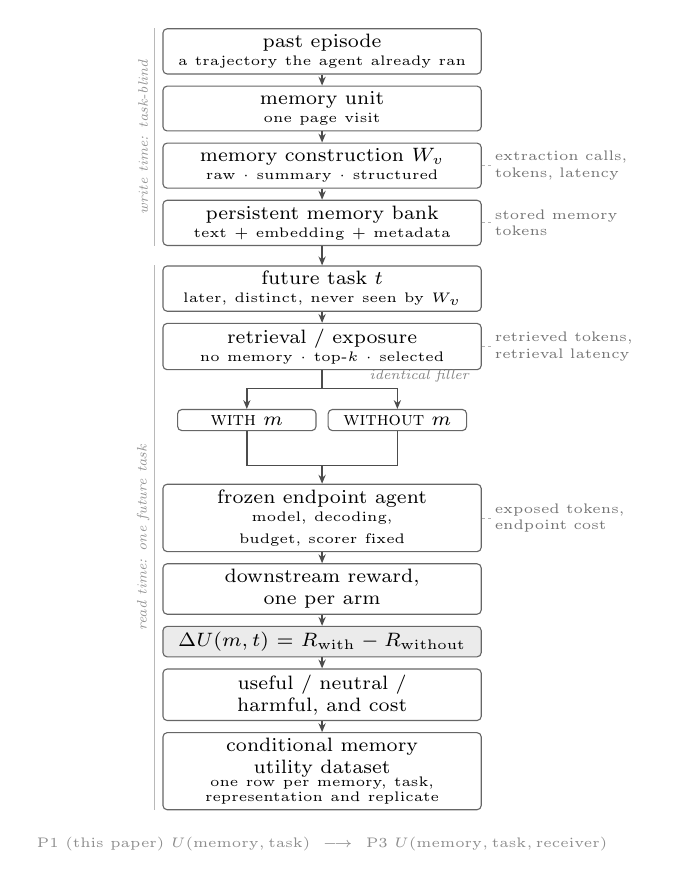
\begin{tikzpicture}[
  font=\scriptsize,
  box/.style={draw=black!60, rounded corners=1.5pt, align=center,
              inner xsep=2.5pt, inner ysep=2.0pt, line width=0.4pt, fill=white},
  spine/.style={box, text width=110pt},
  arm/.style={box, text width=45pt},
  flow/.style={-{Stealth[length=3.2pt,width=2.6pt]}, draw=black!70, line width=0.5pt},
  plain/.style={draw=black!70, line width=0.5pt},
  cost/.style={align=left, font=\tiny, text=black!55, text width=60pt, inner sep=0.5pt},
  tie/.style={draw=black!30, line width=0.3pt, dash pattern=on 1pt off 1.2pt},
  lbl/.style={font=\tiny\itshape, text=black!50, inner sep=1pt},
  phase/.style={font=\tiny\itshape, text=black!42, inner sep=0pt, rotate=90},
]
\def\g{4.0pt}
\hyphenpenalty=10000 \exhyphenpenalty=10000 \sloppy
% ================= WRITE TIME =================
\node[spine] (ep) {past episode\\[-1.5pt]{\tiny a trajectory the agent already ran}};
\node[spine, below=\g of ep] (unit) {memory unit\\[-1.5pt]{\tiny one page visit}};
\node[spine, below=\g of unit] (write)
  {memory construction $W_v$\\[-1.5pt]{\tiny raw $\cdot$ summary $\cdot$ structured}};
\node[spine, below=\g of write] (bank)
  {persistent memory bank\\[-1.5pt]{\tiny text $+$ embedding $+$ metadata}};
\draw[flow] (ep)--(unit); \draw[flow] (unit)--(write); \draw[flow] (write)--(bank);
% ================= READ TIME =================
\node[spine, below=7pt of bank] (task)
  {future task $t$\\[-1.5pt]{\tiny later, distinct, never seen by $W_v$}};
\node[spine, below=\g of task] (ret)
  {retrieval / exposure\\[-1.5pt]{\tiny no memory $\cdot$ top-$k$ $\cdot$ selected}};
\draw[flow] (bank)--(task); \draw[flow] (task)--(ret);
% ---- the paired contrast ----
\node[arm, below left=14pt and 2pt of ret.south] (with) {\textsc{with} $m$};
\node[arm, below right=14pt and 2pt of ret.south] (without) {\textsc{without} $m$};
\coordinate (sp) at ($(ret.south)+(0,-6.5pt)$);
\draw[plain] (ret.south)--(sp);
\draw[flow] (sp) -| (with.north);
\draw[flow] (sp) -| (without.north);
\node[lbl, anchor=west] at ($(sp)+(16pt,4.5pt)$) {identical filler};
\node[spine, below=14pt of ret.south, yshift=-27pt] (agent)
  {frozen endpoint agent\\[-1.5pt]{\tiny model, decoding, budget, scorer fixed}};
\coordinate (jn) at ($(agent.north)+(0,6.5pt)$);
\draw[plain] (with.south)|-(jn); \draw[plain] (without.south)|-(jn);
\draw[flow] (jn)--(agent.north);
\node[spine, below=\g of agent] (rew) {downstream reward, one per arm};
\draw[flow] (agent)--(rew);
\node[spine, below=\g of rew, fill=black!8] (du)
  {$\Delta U(m,t)=R_{\text{with}}-R_{\text{without}}$};
\draw[flow] (rew)--(du);
\node[spine, below=\g of du] (lab) {useful / neutral / harmful, and cost};
\draw[flow] (du)--(lab);
\node[spine, below=\g of lab] (ds)
  {conditional memory utility dataset\\[-1.5pt]{\tiny one row per memory, task,\\[-2.5pt]representation and replicate}};
\draw[flow] (lab)--(ds);
% ================= EFFICIENCY RAIL =================
\node[cost, right=4pt of write.east, anchor=west] (c1) {extraction calls,\\tokens, latency};
\node[cost, right=4pt of bank.east, anchor=west] (c2) {stored memory\\tokens};
\node[cost, right=4pt of ret.east, anchor=west] (c3) {retrieved tokens,\\retrieval latency};
\node[cost, right=4pt of agent.east, anchor=west] (c4) {exposed tokens,\\endpoint cost};
\draw[tie] (write.east)--(c1.west); \draw[tie] (bank.east)--(c2.west);
\draw[tie] (ret.east)--(c3.west);   \draw[tie] (agent.east)--(c4.west);
% ================= PHASE BRACKETS =================
\draw[draw=black!28, line width=0.4pt] ($(ep.north west)+(-3pt,0)$) -- ($(bank.south west)+(-3pt,0)$);
\node[phase] at ($(ep.north west)!0.5!(bank.south west)+(-7pt,0)$) {write time: task-blind};
\draw[draw=black!28, line width=0.4pt] ($(task.north west)+(-3pt,0)$) -- ($(ds.south west)+(-3pt,0)$);
\node[phase] at ($(task.north west)!0.5!(ds.south west)+(-7pt,0)$) {read time: one future task};
% ================= FOOTER (visually secondary) =================
\node[below=6pt of ds.south, font=\tiny, text=black!45, align=center]
  {P1 (this paper) $U(\text{memory},\text{task})\ \longrightarrow\ $ P3 $U(\text{memory},\text{task},\text{receiver})$};
\end{tikzpicture}
\caption{The conditional memory utility protocol. At \emph{write time} a past
episode is cut into naturally occurring memory units and written down in three
representations by a writer that never observes a future task. At \emph{read
time} each memory is paired with several distinct later tasks and evaluated by
paired re-execution of a frozen reader --- identical controlled filler in both
arms, the \textsc{with} arm adding exactly one item --- so the measured
quantity is a signed $\Delta U(m,t)$ per cell, not one score per memory.
Efficiency quantities (right) sit on the same row as the utility they paid
for, including the cost of \emph{forming} the memory.}
\label{fig:pipeline}
\end{figure}

\section{Conditional Memory Evaluation}
\label{sec:method}
%%% Sources: docs/MEMORY_PROTOCOL.md (frozen), docs/ANALYSIS_PREREGISTRATION.md
%%% (fixed before any data existed -- git history proves the ordering),
%%% docs/MEMORY_REPRESENTATIONS.md (B's implementation + B6 pilot).

\subsection{The measured quantity}
Figure~\ref{fig:pipeline} gives the protocol end to end.
For a memory $m$ formed from a past episode and a later, distinct future task
$t$, executed under seed $s$:
\begin{equation}
\label{eq:du}
  \Delta U(m, t, s) \;=\; R\!\left(t \mid m \text{ available}; s\right)
                        \;-\; R\!\left(t \mid m \text{ absent}; s\right),
\end{equation}
where both arms fix the reader model, cluster, serving configuration,
decoding, prompt scaffold, context budget, and scoring function and version,
differing only in the availability of $m$. Reward stays continuous wherever
the benchmark gives partial credit, and the per-cell estimate is the mean over
replicates with a bootstrap interval. The unit of analysis is the cell
$(m,t)$: a memory has no single utility here, so its result is its profile
across the tasks it faced.

\subsection{Identical controlled filler, and the leakage invariant}
Eq.~\eqref{eq:du} removes one memory, which is only what it measures if the
surrounding context is constant: both arms place the same fixed controlled
filler in the reader's context and the WITH arm adds $m$, so the WITHOUT arm is
not an empty-context arm. A measurement forced this. On LongMemEval's first
version~\cite{lmev1} the oracle context is \textbf{entirely evidence} --- a
median $6{,}913$ tokens of context of which a median $6{,}913$ is evidence ---
so ablating ``the memory'' there deletes the whole context and answers a
different question.
%%% VERIFIED: docs/DATASET_FEASIBILITY.md Sec. 3 (the median-token measurement),
%%% corroborated in docs/MEMORY_PROTOCOL.md and docs/MEMORY_UNIT_LMEV2.md.
%%% CORRECTED 2026-10-01: this previously read "948 of 948 ... zero filler" and
%%% cited LEAKAGE_AUDIT.md. That doc reports 471/948 labelled evidence and
%%% 22,919 filler sessions -- those are the DETECTOR's flag rates over the V1
%%% corpus, a different quantity from the ORACLE CONTEXT's composition. No
%%% artifact states 948/948, and the comment claiming it was "positive-
%%% controlled by direct count" was false. The claim itself survives in its
%%% measured form; only the unsourced count is gone.
On our primary benchmark the intervention is measured to be local
(Section~\ref{sec:setup}). This also answers the fair-comparison
critique~\cite{memoryrtwo}: the memory set is written once, frozen and
content-hashed before any pairing exists, no arm writes, updates or deletes a
memory, and the arms differ by exactly one item from that frozen set, so no
divergent intermediate state exists.

Memory formation is a function of the past episode alone, $m = W_v(e)$ and
never $m = W_v(e,t)$. Without this, $\Delta U(m,t) > 0$ shows only that a model can be told the
answer and copy it forward, and every conditional claim collapses. It is the
assumption to attack first, so we enforce it structurally with four
barriers --- \textbf{arity} (a writer takes a segment
and nothing else), \textbf{a closed field set}, \textbf{a metadata denylist}
(the weakest, present only to make a plumbing mistake loud), and \textbf{a
single interpolation point} (one placeholder, the segment text) --- each
carrying a negative control that plants the defect and requires the check to
fire. Prompt identity derives from the file bytes, not a hand-maintained
constant that can report a stale version.

\paragraph{The bearing criterion is a measurement instrument, not a
retrieval policy.}
%%% TASK 4 (SA-SCI-PAPER), read off the CODE, not the prose:
%%%   scripts/k1_build_screened_design.py -> LK.detect(memory_text, t.answer,
%%%   eval_function_spec=t.eval_function) in src/p1mem/adapters/leakage.py.
%%% The three inputs are (i) the memory text, (ii) the task's GOLD ANSWER,
%%% (iii) the task's eval-function spec. The question text is NEVER passed --
%%% grep for `.question` in leakage.py returns nothing. So the screen reads
%%% benchmark ground truth that no deployed retriever has, and the paper must
%%% say so in those words rather than leaving a reviewer to infer it from
%%% "contains what the task needs".
The same scorer drives a \emph{screen} we use to decide which (memory, task)
pairs are worth executing, and its inputs must be stated exactly, because
they are not the inputs a retriever would have. For each pair it receives
three things: the memory's rendered text, the task's \textbf{gold answer},
and the task's evaluation-function specification. It never sees the question,
and no reward, model output or outcome of any kind enters it --- which is why
the resulting strata are not selected on the outcome. A pair is
\textsc{bearing} when the benchmark's own scorer would mark the memory text
correct against that gold answer \emph{and} the same test singles this memory
out of its whole same-domain pool, firing on at most eight of the
$865$--$1{,}024$ units available to that task; a detector firing on two dozen
of two dozen has said nothing about any of them, which an earlier
non-discriminative version of this flag did, at a ratio of $0.995$ between
paired and unpaired memories.

\textbf{This is a measurement instrument, not a deployable retrieval policy.}
It consumes the gold answer, which is exactly what a deployed system does not
have, so it cannot be used to retrieve and we do not propose it as a
retriever. Its purpose is the opposite: by locating, with ground truth, the
pairs on which a memory actually bears, it exposes the quantity that a future
retrieval or gating method would have to approximate without ground truth ---
and makes visible how far a generic similarity retriever is from
approximating it (Section~\ref{sec:similarity}). Every rate we report under
it is therefore conditional on a screened design and is never a natural base
rate.

\textbf{A screen that never sees the gold answer finds the same effect.} The
objection this instrument invites is that a cell selected because the memory
carries the answer is a cell where a memory trivially helps. We tested it
directly. Two \emph{gold-free} screens were pre-registered before execution,
each reading the memory, the question and the same-domain pool, and none of
the gold answer, the reward, any model output or the evaluation
specification. On the cells the gold screen \emph{never} selected, the
gold-free bearing set moves the reader from $\gfWithoutPct$\% correct without
the memory to $\gfWithPct$\% with it ($n{=}\gfN$ rows), while its matched
control does not improve at all ($\gfCtlWithoutPct$\% to
$\gfCtlWithPct$\%); the contrast is $\gfDiff$ over $\gfCells$ cells. The
effect therefore does not depend on answer containment, and it is not an
artifact of selecting cells on ground truth.

We report \emph{both} gold-free screens, including the one that found
nothing, because reporting only the screen that worked would select an
instrument on its outcome. A purely lexical variant returns no effect, and a
diagnostic independent of any utility says why it should not be believed: its
bearing cells fail in both arms at $\gfLexBaf$, \emph{worse} than unscreened
random pairing, against $\gfLlmBaf$ for the screen above. A criterion whose
selections are harder than a random draw has not located bearing. The
surviving estimate rests on $\gfCells$ cells and is cross-session against the
gold run, so it agrees with it in sign and significance rather than in
magnitude.

The invariant excludes \emph{task-directed writing}, not a naturally
occurring memory that happens to contain a later answer: that is a real memory
being genuinely useful, and removing those cells would condition the cell set
on the outcome. We audit every cell with a detector reusing the benchmark's
own scorer, asking whether the rendered memory text alone would score correct
against the gold answer, and we flag rather than filter. It is validated by 17
controls --- plants it must catch, clean cases it must not fire on, two pinned
known false negatives --- and aborts if any fails.
%%% VERIFIED: docs/LEAKAGE_AUDIT.md. 17/17; two failed on first run, both
%%% control-construction errors, one exposing a real bug in the OFFICIAL scorer
%%% (see Limitations).

\subsection{Three representations of the same experience}
All three derive from the \emph{same} source segment, bound once and handed
to each writer, so any downstream difference is attributable to representation
rather than content selection. \textbf{Raw/extractive} is deterministic and
uses no model: the memory \emph{is} the segment, whose boundaries were drawn
upstream by the past agent's own behaviour, with no span selection ---
``pick the most informative span'' would smuggle in the value judgement the
experiment exists to measure. \textbf{Abstractive summary} is one call per
segment at pinned decoding and prompt version. \textbf{Structured experience}
is one call emitting a validated schema (\emph{memory type $\cdot$ trigger
$\cdot$ action $\cdot$ outcome $\cdot$ lesson $\cdot$ scope}, with a
procedural variant substituting \emph{trigger $\cdot$ procedure $\cdot$
failure mode $\cdot$ correction $\cdot$ scope}); a malformed structure is a
recorded failure, never repaired and never a silent fallback to prose --- a
repaired structure is a different structure --- and the malformed text is
retained, since a discarded failure cannot be audited. Representation is
orthogonal to \emph{semantic type}: the dataset carries them separately and we
report labelling-pass agreement rather than presenting type as given
(Section~\ref{sec:limitations}).

\paragraph{Formation cost belongs to the representation.}
Raw costs zero calls; summary and structured cost one each per segment. An
efficiency comparison omitting formation cost flatters the model-written
representations, so each is charged its own, and we distinguish three
routinely merged zeros: a measured zero (raw makes zero extraction calls), an
absent measurement (no call was made, so the cell leaves that denominator),
and an unreported field (the endpoint exposes no counter). Failed writes
count --- one that failed after burning a call still cost it.

\section{Benchmarks and Experimental Setup}
\label{sec:setup}
%%% Sources: docs/BENCHMARK_DECISIONS.md, docs/MEMORY_UNIT_LMEV2.md,
%%% docs/CLUSTER_DECISION.md, docs/INFRA_VERIFICATION.md, docs/POWER_ANALYSIS.md,
%%% docs/BENCHMARK_LICENSES.md. Every number is in docs/RESULTS_LEDGER.md or in
%%% the cited measurement document with its artifact path.

Eq.~\eqref{eq:du} requires that the same memory be evaluable against several
distinct future tasks. We measured that axis on each candidate benchmark
before committing, and the measurements changed the plan.

\paragraph{LongMemEval-V2, and the page-visit memory unit.}
We use the \texttt{small} tier of LongMemEval-V2~\cite{lmev2}, where each
domain has exactly one haystack --- identical across questions even as an
ordered tuple --- so every memory is legitimately available to every question
in its domain, with no availability confound between arms; the same test
returns 222 and 211 distinct haystacks on \texttt{medium}, the positive
control showing it distinguishes the two cases. A whole trajectory cannot be
a memory: under the benchmark's own tokenizer over 200 trajectories and 5,095
states the median trajectory is 103,886 tokens. We segment at the \emph{page visit}, the maximal run of consecutive states
sharing one URL --- a boundary drawn by the past agent's own navigation, by a
function taking a trajectory and nothing else. This yields \textbf{1,889
memory units}, median \textbf{7,261 tokens}.
%%% VERIFIED: docs/MEMORY_UNIT_LMEV2.md Sec. 2; reproducible with
%%% scripts/build_lmev2_units.py --tier small --seed 20261008.
Two measured properties make this a memory rather than a context ablation:
removing one unit removes a median 3.33\% of its trajectory and 0.058\% of the
domain haystack, and segmentation preserves answerability for 94.2\% of
deterministically scored questions (278 of 295).

\paragraph{Future tasks, pairing, and power.}
A future task is one question with its evaluation-function specification. Of
451 questions, \textbf{295 are deterministically scored} and 156 need an LLM
judge. There are \emph{eight} distinct specification strings, not six --- two
phrase-match variants differ only in their separator --- so our adapter
dispatches on the full string, never the function name, and uses the
benchmark's scorer verbatim: its phrase matcher is gold-phrase
\emph{containment}, not set equality, which a name-based reimplementation gets
wrong. An LLM-judged task \emph{raises} rather than returning a default, since
a silent \texttt{False} would turn ``cannot evaluate'' into ``wrong answer''
for 156 of 451 questions in both arms. Seeded deterministic pairing within
domain, stratified by the benchmark's own question-type taxonomy, gives
\textbf{1,889 memories $\times$ 8 tasks $=$ 15,112 cells}, every memory
verified to get exactly 8; the build asserts the same seed reproduces
byte-identically \emph{and} that a different seed differs, so reproducibility
is not vacuous. That grid is the available pairing, not the executed design
(Table~\ref{tab:coverage}). We fixed a floor of \textbf{60 memories} before
running, from a recovery study on synthetic data with known planted components
that also showed widening the task axis beats adding memories. The executed
design meets it; Section~\ref{sec:metrics} reports why the decomposition it
was sized for is not estimable on a reader deterministic within a session.
%%% VERIFIED: docs/POWER_ANALYSIS.md, measured with
%%% src/p1mem/analysis/decomposition.py over 6 seeds; reproduction snippet there.

\paragraph{BEAM demoted; two secondary benchmarks, each reported at its own
strength.}
BEAM~\cite{beam} was in our frozen plan as the multi-domain check but cannot
supply the axis: \textbf{92.6\% of its cited turns are cited by exactly one
question}, so the same memory is almost never evaluated against two tasks. We
demote it on that measurement rather than on the schedule; being CC~BY-SA~4.0
it would also ship separately, since ShareAlike would otherwise relicense the
rest.

The two benchmarks we did execute are secondary in different ways
(Table~\ref{tab:coverage}). In SciCode~\cite{scicode} the unit is a reusable
helper routine with its procedure, transferring \emph{across} problems;
against an early feasibility estimate of 8--12 pairs, the whole candidate pool
measured on the built adapter is \textbf{\sciPairs{} donor$\to$recipient
pairs} (\sciMems{} memories, \sciTasks{} tasks), and we ran all of it. On
SWE-bench Verified~\cite{swebench} the pairing is likewise excellent but the
\emph{measurable} yield is not: across \covSwRepos{} repositories, after a
localizer that misses the edit region on \sweLocMiss{} cells and edits that
neither apply nor produce a test verdict, \textbf{\sweMatched{} cells} are
interpretable under all three representations, \sweDomRepoPct\% from one
repository --- a two-repository result dominated by one. A scoring defect we
corrected is part of that count: a suite that printed no verdict at all --- an
import or collection error --- was recorded as a reward of zero. Demoting
those $37$ arm-reads to unscorable moves the matched set from $17$ to
\sweMatched{}; every contrast crosses zero before and after.

\textbf{Neither secondary benchmark establishes an ordering}; we report that
as a boundary on the primary result in Section~\ref{sec:crossbench} rather
than as a second confirmation of it.


%%% ============ TABLE 2: COVERAGE ==========================================
%%% EVERY NUMBER GENERATED into figdata.tex by scripts/make_figures.py.
%%% Each of the three terms is counted from its OWN source -- eligible from
%%% the pre-committed design manifest or the pair design, attempted and
%%% completed from the executed row files, excluded from the rows that could
%%% not be scored -- so the identity eligible = completed + excluded is a
%%% CHECK rather than an arithmetic restatement.
%%%
%%% 🔴 THIS TABLE'S OWN GUARD WAS FOUND VACUOUS BY PLANTING THE DEFECT.
%%% A first version derived `eligible` as completed + excluded, which made
%%% the closing identity unable to fail: deleting an entire exclusion
%%% category closed just as neatly as a complete run. Found by
%%% scripts/verify_figure_guards.py plant [M]. Every term is now counted
%%% independently, and plants [M], [S], [T] confirm the identity can break.
%%%
%%% THE UNIVERSE MUST BE NAMED (docs/COVERAGE_MANIFEST.md). LongMemEval's
%%% row is the screened design the paper reports, which is 1,157 cells. The
%%% frozen 15,112-pair grid is a DIFFERENT universe and the table says so in
%%% the caption; quoting either percentage without naming its universe is
%%% false against the other.
\begin{table}[t]
\centering\small
\caption{Coverage, on the universe each result is reported over. Cells are
(memory, task, representation); a cell is \textsc{excluded} when no reward
could be produced --- unscorable execution, localizer miss, memory never
written --- and is never recorded as a reward of zero. The columns come from
separate artifacts, so \textsc{eligible} $=$ \textsc{completed} $+$
\textsc{excluded} is a check the build can fail. LongMemEval-V2's universe is
the screened design we report; the frozen grid it was re-drawn from holds
15,112 pairs, and a percentage is false against one of the two unless the
universe is named.}
\label{tab:coverage}
\setlength{\tabcolsep}{4pt}
\begin{tabular}{@{}lrrrr@{}}
\toprule
benchmark & eligible & completed & excluded & \% \\
\midrule
LongMemEval-V2 & \covLmElig & \covLmDone & \covLmExcl & \covLmPct \\
SciCode        & \covScElig & \covScDone & \covScExcl & \covScPct \\
SWE-bench      & \covSwElig & \covSwDone & \covSwExcl & \covSwPct \\
\bottomrule
\end{tabular}
\end{table}

\textbf{SWE-bench content is not redistributed.} The harness is MIT, but the
\texttt{SWE-bench\_Verified} corpus declares \emph{no} licence --- none in its
hub metadata, no tag, no statement on its card --- and its issue text and
patches belong to the upstream projects. Our release therefore carries
SWE-bench instance identifiers and our own derived measurements only, every
source-text field withheld and marked as withheld. An absent licence is not a
permissive one, and the exporter enforces this rather than convention.

\paragraph{Frozen execution configuration.}
Cluster and serving configuration are experimental identity, so every row
records the full pinned set --- in the primary arms reader and memory writer
are both \texttt{gpt-oss-120b} on one cluster, \texttt{reasoning\_effort} low,
temperature 0, \texttt{max\_tokens} 512, 16 concurrent workers,
SFR-Embedding-Mistral at dim 4096, the benchmark's own tokenizer --- and a
change to any of them defines a new arm rather than additional data.
Section~\ref{sec:readertransfer} changes the reader to
\texttt{gemma-4-31B-it}, and \emph{only} the reader, on that basis; model
identity stays explicit wherever a cost is reported, since the two do not
expose the same token-accounting categories. Three settings were fixed by
measurement, each guarding a way the study could have produced numbers that
looked fine: an empty or truncated completion raises and the cell is re-run
rather than scoring zero, which would push $\Delta U$ negative and
\emph{manufacture} the harmful memories we set out to measure; concurrency
sits at a measured saturation ceiling, with the ladder pushed past the chosen
value, since a ceiling cannot be justified without observing one; and
responses are cached on all twelve fields of a cell's experimental identity,
verified behaviourally by varying one field and confirming a miss.

\section{Metrics}
\label{sec:metrics}
%%% Source: docs/ANALYSIS_PREREGISTRATION.md, committed BEFORE any experimental
%%% data existed -- git history proves the ordering. Every threshold below was
%%% chosen without having seen a single Delta-U value; changing one after results
%%% exist requires a DECISION_LOG entry and BOTH numbers appear in the paper.

\subsection{Utility, floors, and robust labels}
We neither threshold reward where partial credit exists nor reduce a memory
to a scalar. Both a flip rate and an interaction share are
threshold-dependent, so a threshold chosen after seeing data turns any noisy
measurement into a finding; ours were fixed before data existed, and the
floors measured first. Three floors, not interchangeable: $F_{\mathrm{exec}}$,
outcome variation across seeds with everything else fixed (the reference
floor, per benchmark, with a bootstrap interval), measured \emph{within a
single execution session}, since this endpoint is not stable across days
(Section~\ref{sec:limitations}); $F_{\mathrm{empty}}$, variation of the
no-memory arm, free because that arm is identical across every memory
condition for a task; and $F_{\mathrm{judge}}$, scorer disagreement on
\emph{byte-identical} outputs from re-scoring stored generations. The last
should be near zero for deterministic scorers --- one reason we prefer them
--- but is measured: a prior study in our group saw a 9.35\% verdict flip rate
on byte-identical inputs at temperature~0. We store full output text rather
than a digest so this re-scoring is possible.

The floor is on the $\Delta U$ scale, not per arm: since
$\mathrm{var}(\Delta U) = \mathrm{var}_{\mathrm{with}} +
\mathrm{var}_{\mathrm{without}} - 2\,\mathrm{cov}$, only the contrast scale is
comparable to a mean $\Delta U$; per-arm floors are reported alongside. One hazard would fabricate the whole result: the WITHOUT arm's inputs are
identical across memories, so a cache serving it would reuse one generation
everywhere and let every $\Delta U$ clear a zero floor. That arm is
re-generated per (task, replicate), and a measured $F_{\mathrm{empty}} = 0$
raises rather than passes.

Let $\mathrm{CI}(m,t)$ be the 95\% bootstrap interval of mean $\Delta U$ over
replicates and $F$ the floor. A cell is \textbf{robust useful} when
$\mathrm{CI}_{\mathrm{lower}} > 0$ \emph{and} $\overline{\Delta U} > F$;
\textbf{robust harmful} when $\mathrm{CI}_{\mathrm{upper}} < 0$ \emph{and}
$|\overline{\Delta U}| > F$; \textbf{neutral} otherwise --- both clauses, so a
cell can be statistically nonzero and still neutral. A memory shows a
\textbf{robust sign flip} iff two of its cells are respectively robust useful
and robust harmful, each independently clearing the criterion, so a raw sign
difference is not a flip. Any flip rate carries its denominator (memories on $\ge 2$ tasks) and a
Wilson interval beside the naive no-floor rate, and a cell needs $\ge 2$
replicates to enter one, since a single-replicate pilot yields a headline of
exactly zero whatever the truth.

\paragraph{A sign flip is not evidence of interaction.}
%%% BINDING: docs/ANALYSIS_PREREGISTRATION.md Amendment A1.1 and the matching
%%% forbidden-claim clause in docs/LITERATURE_BOUNDARY.md. Any sentence of the
%%% form "memories flip sign, therefore utility is task-conditional" is FALSE
%%% and forbidden, whatever the measured rate. This paragraph is the correction.
We state this before any data, because it decides the headline. A flip is a
property of $\Delta U$'s \emph{sign}; interaction is a property of its
\emph{variance}, and the first does not imply the second. Under a purely
\emph{additive} model $\Delta U(m,t) = \mu + a_m + b_t$ with the interaction
identically zero, a memory still helps one task and harms another whenever
$b_t$ crosses $-(\mu + a_m)$: simulating that null over 20 trials of 200
memories $\times$ 8 tasks gives sign-flip rates of \textbf{53.5\%--92.0\%}
with \emph{zero} interaction present.
%%% VERIFIED: docs/ANALYSIS_PREREGISTRATION.md A1.1 table (Master Agent, 20
%%% trials x 200 memories x 8 tasks): 0.749 / 0.920 / 0.535 / 0.718 / 0.645
%%% across the five (mu, sd_memory, sd_task) settings. Sub-agent D independently
%%% measured 0.598 under its own generative settings.
A high flip rate is therefore fully consistent with memory value being a
scalar plus a task-difficulty term, so we report it as a \textbf{descriptive,
operational} fact --- a single scalar cannot tell you the sign for a given
task --- and never as evidence of interaction. Our pre-registered standard for
a conditionality claim required two quantities together; neither is available
on this design, and Section~\ref{sec:r0} reports why.

\subsection{Decomposition, distance, and efficiency}
%%% REWRITTEN. The pre-registered plan was to report component variance shares.
%%% It is NOT estimable on this design and no such share is quoted anywhere in
%%% this paper (docs/ADDITIVE_NULL_AND_DECOMPOSITION.md Sec. 2: F_exec = 0,
%%% fitted residual 3.07e-06, task and interaction shares equal to 16 s.f.
%%% pinned at the optimizer's clip while reporting converged=True). The
%%% identifiability PRECONDITION was recorded in docs/IDENTIFIABILITY_STATUS.md
%%% BEFORE the run, which is why this states the failure as a predicted outcome
%%% of a measured structural property rather than discovering it afterwards.
We pre-registered a decomposition of $\Delta U(m,t,s) = \mu + a_m + b_t +
(ab)_{mt} + \varepsilon_s$ into component variance shares against
$F_{\mathrm{exec}}$, with a method-of-moments fallback fixed in advance so
non-convergence would be disclosed rather than silently swapped. We recorded
the structural precondition before executing: components are identified only
relative to a residual scale. It fails here, for a reason the rest of the
design makes desirable --- our reader is deterministic within a session ---
so \textbf{we quote no such share}, and Section~\ref{sec:r0} treats the
failure as a result about what a noiseless reader costs. Standard errors are
clustered by task throughout. Semantic distance is
$\cos(\mathrm{embed}(m),\mathrm{embed}(t))$ under the pinned embedding model,
whose determinism we verified directly (cosine of identical texts exactly
1.0), banded by terciles fixed before outcomes are examined, since cosine
scales are not comparable across corpora. We report Spearman correlation
between similarity and mean utility, overall and per band, against the content
criterion of Section~\ref{sec:method} --- as measurement, not discovery: that
relevance is not utility is already stated in prior work.

Every utility measurement is paired with its cost in seven families:
\textbf{storage} (memory tokens held), \textbf{retrieval} (latency, tokens
returned), \textbf{exposure} (tokens placed in the reader's context),
\textbf{generation} (latency, input, output, reasoning tokens),
\textbf{extraction} (formation cost), \textbf{API and compute}, and
\textbf{selectivity} (how much of what was retrieved was worth exposing).
Exposure is deliberately distinct from retrieval: the gap is truncation loss,
invisible if only one is recorded. The central quantity is \textbf{exposure
efficiency}, utility per exposed token, since exposed tokens are what the
reader pays for and what a retention policy controls; each representation is
additionally charged its own formation cost, so one cheap to store but
expensive to write does not appear free. A cost family is reported per model
and never summed across models, since two models need not expose the same
counters.

\section{Results}
\label{sec:results}
%%% RESTRUCTURED 2026-10-01 (SA-SCI-PAPER). The headline results previously
%%% sat UNDER \section{Limitations}, which inverted the paper: a reader met
%%% the caveats before the findings. They are MOVED here -- every number, CI,
%%% denominator and caveat travels with its own sentence. Nothing was
%%% re-derived, re-rounded or re-worded in the move; `scripts/audit_claims.py`
%%% is the check on that, since it re-derives the CIs, the strata, the reader
%%% effect and the required caveat strings from the tracked artifacts and
%%% fails if one went missing. Several caveats below exist because an
%%% instrument defect was found (docs/DEFECT_REGISTER.md) -- deleting one
%%% deletes the evidence, not the hedge.
%%%
%%% ORDER = the contribution hierarchy of Sec. 1: sparsity (B) -> the screen
%%% that makes it measurable (A) -> what fails to locate it -> representation
%%% and cost (C) -> the cross-benchmark bound (E) -> reader generalization (D)
%%% -> the founding negative, LAST, because it is evidence about the
%%% instrument and not a peer contribution.
%%%
%%% WHAT STAYS IN LIMITATIONS: only genuine limits -- the constructed pairing,
%%% the official-scorer bug that makes leakage a lower bound, cross-session
%%% drift, the two abandoned axes, the single cluster and domain.

%%% ===================== FIGURE 2: scarcity and sign reversal =====================
%%% EVERY NUMBER IN THIS FIGURE IS GENERATED, NOT TYPED. The bar heights, the
%%% interval endpoints and the counts all come from %%% GENERATED by scripts/make_figures.py in the code repository.
%%% DO NOT EDIT BY HAND, and do not edit a value here to make a
%%% figure look right -- regenerate. Every value is recomputed from
%%% a tracked artifact and cross-checked against the audited value;
%%% the generator exits non-zero on any disagreement, and a planted
%%% sign flip in one BEARING cell is verified to make it fail.
%%% Sources: data/manifests/lmev2_leakage_small.jsonl
%%%          results/ledgers/repro/screened_cells_slim.jsonl
%%%          results/ledgers/k1_screened_design.json (basis pin)

%% --- sparsity map (fig 1b): one square per MEASURED cell ---
%% The paper's central claim, drawn at cell level. dU is exactly
%% three-valued (-1/0/+1) and the generator FAILS if a fourth
%% level appears. Unmeasured slots are drawn as NOTHING: the
%% rows are ragged, and padding them to a rectangle collapses
%% the BEARING/RANDOM contrast from 3.83x to 1.02x -- both
%% readings are asserted so a padded redraw cannot pass.
\def\spPos{0.00/0.00,4.20/0.00,8.40/0.00,46.80/0.00,93.60/0.00,0.00/-2.55,4.20/-2.55,8.40/-2.55,46.80/-2.55,93.60/-2.55,0.00/-5.10,4.20/-5.10,8.40/-5.10,46.80/-5.10,93.60/-5.10,97.80/-5.10,0.00/-7.65,4.20/-7.65,8.40/-7.65,93.60/-7.65,97.80/-7.65,0.00/-10.20,4.20/-10.20,46.80/-10.20,51.00/-10.20,0.00/-12.75,4.20/-12.75,93.60/-12.75,0.00/-15.30,4.20/-15.30,93.60/-15.30,97.80/-15.30,0.00/-17.85,4.20/-17.85,0.00/-20.40,4.20/-20.40,0.00/-22.95,4.20/-22.95,93.60/-22.95,0.00/-25.50,4.20/-25.50,93.60/-25.50,97.80/-25.50,102.00/-25.50,0.00/-28.05,4.20/-28.05,93.60/-28.05,97.80/-28.05,102.00/-28.05,0.00/-30.60,4.20/-30.60,93.60/-30.60,97.80/-30.60,0.00/-33.15,4.20/-33.15,93.60/-33.15,0.00/-35.70,46.80/-35.70,93.60/-35.70,0.00/-38.25,0.00/-40.80,93.60/-40.80,0.00/-43.35,0.00/-45.90,93.60/-45.90,97.80/-45.90,0.00/-48.45,93.60/-48.45,97.80/-48.45,0.00/-51.00,93.60/-51.00,0.00/-53.55,93.60/-53.55,0.00/-56.10,93.60/-56.10,97.80/-56.10,102.00/-56.10,0.00/-58.65,93.60/-58.65,0.00/-61.20,93.60/-61.20,97.80/-61.20,0.00/-63.75,46.80/-63.75,93.60/-63.75,0.00/-66.30,0.00/-68.85,93.60/-68.85,0.00/-71.40,93.60/-71.40,97.80/-71.40,0.00/-73.95,0.00/-76.50,46.80/-76.50,93.60/-76.50,97.80/-76.50,102.00/-76.50,106.20/-76.50,0.00/-79.05,93.60/-79.05,97.80/-79.05,93.60/-81.60,93.60/-84.15,97.80/-84.15,93.60/-86.70,93.60/-89.25,97.80/-89.25,93.60/-94.35,97.80/-94.35,46.80/-96.90,93.60/-96.90,97.80/-96.90,102.00/-96.90,93.60/-99.45,93.60/-102.00,93.60/-104.55,97.80/-104.55,93.60/-107.10,93.60/-109.65,97.80/-109.65,93.60/-112.20,93.60/-114.75,93.60/-117.30,97.80/-117.30,93.60/-119.85,93.60/-122.40,93.60/-124.95,93.60/-127.50,93.60/-130.05,97.80/-130.05,102.00/-130.05,46.80/-132.60,93.60/-135.15,93.60/-137.70,93.60/-140.25,97.80/-140.25,93.60/-142.80,93.60/-145.35,93.60/-147.90,93.60/-150.45,97.80/-150.45,102.00/-150.45}
\def\spNeg{59.40/-7.65,152.40/-7.65,80.40/-10.20,139.80/-10.20,67.80/-15.30,148.20/-15.30,152.40/-17.85,148.20/-28.05,148.20/-38.25,152.40/-38.25,144.00/-45.90,148.20/-45.90,152.40/-45.90,152.40/-48.45,148.20/-51.00,46.80/-53.55,144.00/-61.20,148.20/-61.20,148.20/-66.30,152.40/-66.30,152.40/-71.40,152.40/-79.05,12.60/-81.60,55.20/-84.15,55.20/-86.70,4.20/-99.45,152.40/-114.75,148.20/-117.30,152.40/-122.40,152.40/-124.95,152.40/-130.05,152.40/-137.70,152.40/-142.80,152.40/-150.45}
\def\spZero{12.60/0.00,16.80/0.00,21.00/0.00,25.20/0.00,29.40/0.00,33.60/0.00,51.00/0.00,55.20/0.00,59.40/0.00,63.60/0.00,67.80/0.00,72.00/0.00,76.20/0.00,80.40/0.00,97.80/0.00,102.00/0.00,106.20/0.00,110.40/0.00,114.60/0.00,118.80/0.00,123.00/0.00,127.20/0.00,131.40/0.00,135.60/0.00,139.80/0.00,144.00/0.00,148.20/0.00,12.60/-2.55,16.80/-2.55,21.00/-2.55,25.20/-2.55,29.40/-2.55,51.00/-2.55,55.20/-2.55,59.40/-2.55,63.60/-2.55,67.80/-2.55,72.00/-2.55,76.20/-2.55,80.40/-2.55,97.80/-2.55,102.00/-2.55,106.20/-2.55,110.40/-2.55,114.60/-2.55,118.80/-2.55,123.00/-2.55,127.20/-2.55,131.40/-2.55,135.60/-2.55,139.80/-2.55,12.60/-5.10,51.00/-5.10,55.20/-5.10,59.40/-5.10,102.00/-5.10,106.20/-5.10,110.40/-5.10,114.60/-5.10,118.80/-5.10,123.00/-5.10,127.20/-5.10,131.40/-5.10,135.60/-5.10,139.80/-5.10,144.00/-5.10,148.20/-5.10,152.40/-5.10,46.80/-7.65,51.00/-7.65,55.20/-7.65,102.00/-7.65,106.20/-7.65,110.40/-7.65,114.60/-7.65,118.80/-7.65,123.00/-7.65,127.20/-7.65,131.40/-7.65,135.60/-7.65,139.80/-7.65,144.00/-7.65,148.20/-7.65,8.40/-10.20,12.60/-10.20,16.80/-10.20,21.00/-10.20,25.20/-10.20,29.40/-10.20,55.20/-10.20,59.40/-10.20,63.60/-10.20,67.80/-10.20,72.00/-10.20,76.20/-10.20,93.60/-10.20,97.80/-10.20,102.00/-10.20,106.20/-10.20,110.40/-10.20,114.60/-10.20,118.80/-10.20,123.00/-10.20,127.20/-10.20,131.40/-10.20,135.60/-10.20,8.40/-12.75,12.60/-12.75,16.80/-12.75,46.80/-12.75,51.00/-12.75,55.20/-12.75,59.40/-12.75,63.60/-12.75,67.80/-12.75,97.80/-12.75,102.00/-12.75,106.20/-12.75,110.40/-12.75,114.60/-12.75,118.80/-12.75,123.00/-12.75,127.20/-12.75,131.40/-12.75,135.60/-12.75,139.80/-12.75,144.00/-12.75,148.20/-12.75,8.40/-15.30,12.60/-15.30,16.80/-15.30,46.80/-15.30,51.00/-15.30,55.20/-15.30,59.40/-15.30,63.60/-15.30,102.00/-15.30,106.20/-15.30,110.40/-15.30,114.60/-15.30,118.80/-15.30,123.00/-15.30,127.20/-15.30,131.40/-15.30,135.60/-15.30,139.80/-15.30,144.00/-15.30,8.40/-17.85,46.80/-17.85,51.00/-17.85,55.20/-17.85,59.40/-17.85,93.60/-17.85,97.80/-17.85,102.00/-17.85,106.20/-17.85,110.40/-17.85,114.60/-17.85,118.80/-17.85,123.00/-17.85,127.20/-17.85,131.40/-17.85,135.60/-17.85,139.80/-17.85,144.00/-17.85,148.20/-17.85,8.40/-20.40,46.80/-20.40,51.00/-20.40,55.20/-20.40,93.60/-20.40,97.80/-20.40,102.00/-20.40,106.20/-20.40,110.40/-20.40,114.60/-20.40,118.80/-20.40,123.00/-20.40,127.20/-20.40,131.40/-20.40,135.60/-20.40,139.80/-20.40,144.00/-20.40,148.20/-20.40,152.40/-20.40,8.40/-22.95,46.80/-22.95,51.00/-22.95,55.20/-22.95,97.80/-22.95,102.00/-22.95,106.20/-22.95,110.40/-22.95,114.60/-22.95,118.80/-22.95,123.00/-22.95,127.20/-22.95,131.40/-22.95,135.60/-22.95,139.80/-22.95,144.00/-22.95,148.20/-22.95,152.40/-22.95,8.40/-25.50,46.80/-25.50,51.00/-25.50,55.20/-25.50,106.20/-25.50,110.40/-25.50,114.60/-25.50,118.80/-25.50,123.00/-25.50,127.20/-25.50,131.40/-25.50,135.60/-25.50,139.80/-25.50,144.00/-25.50,148.20/-25.50,8.40/-28.05,46.80/-28.05,51.00/-28.05,55.20/-28.05,106.20/-28.05,110.40/-28.05,114.60/-28.05,118.80/-28.05,123.00/-28.05,127.20/-28.05,131.40/-28.05,135.60/-28.05,139.80/-28.05,144.00/-28.05,46.80/-30.60,51.00/-30.60,102.00/-30.60,106.20/-30.60,110.40/-30.60,114.60/-30.60,118.80/-30.60,123.00/-30.60,127.20/-30.60,131.40/-30.60,135.60/-30.60,139.80/-30.60,144.00/-30.60,148.20/-30.60,152.40/-30.60,46.80/-33.15,51.00/-33.15,97.80/-33.15,102.00/-33.15,106.20/-33.15,110.40/-33.15,114.60/-33.15,118.80/-33.15,123.00/-33.15,127.20/-33.15,131.40/-33.15,135.60/-33.15,139.80/-33.15,144.00/-33.15,148.20/-33.15,4.20/-35.70,8.40/-35.70,12.60/-35.70,51.00/-35.70,55.20/-35.70,59.40/-35.70,97.80/-35.70,102.00/-35.70,106.20/-35.70,110.40/-35.70,114.60/-35.70,118.80/-35.70,123.00/-35.70,127.20/-35.70,131.40/-35.70,135.60/-35.70,139.80/-35.70,144.00/-35.70,4.20/-38.25,8.40/-38.25,46.80/-38.25,51.00/-38.25,55.20/-38.25,59.40/-38.25,93.60/-38.25,97.80/-38.25,102.00/-38.25,106.20/-38.25,110.40/-38.25,114.60/-38.25,118.80/-38.25,123.00/-38.25,127.20/-38.25,131.40/-38.25,135.60/-38.25,139.80/-38.25,144.00/-38.25,4.20/-40.80,46.80/-40.80,51.00/-40.80,97.80/-40.80,102.00/-40.80,106.20/-40.80,110.40/-40.80,114.60/-40.80,118.80/-40.80,123.00/-40.80,127.20/-40.80,131.40/-40.80,135.60/-40.80,139.80/-40.80,144.00/-40.80,148.20/-40.80,4.20/-43.35,46.80/-43.35,51.00/-43.35,93.60/-43.35,97.80/-43.35,102.00/-43.35,106.20/-43.35,110.40/-43.35,114.60/-43.35,118.80/-43.35,123.00/-43.35,127.20/-43.35,131.40/-43.35,135.60/-43.35,139.80/-43.35,144.00/-43.35,148.20/-43.35,4.20/-45.90,46.80/-45.90,51.00/-45.90,102.00/-45.90,106.20/-45.90,110.40/-45.90,114.60/-45.90,118.80/-45.90,123.00/-45.90,127.20/-45.90,131.40/-45.90,135.60/-45.90,139.80/-45.90,4.20/-48.45,46.80/-48.45,51.00/-48.45,102.00/-48.45,106.20/-48.45,110.40/-48.45,114.60/-48.45,118.80/-48.45,123.00/-48.45,127.20/-48.45,131.40/-48.45,135.60/-48.45,139.80/-48.45,144.00/-48.45,148.20/-48.45,4.20/-51.00,46.80/-51.00,51.00/-51.00,97.80/-51.00,102.00/-51.00,106.20/-51.00,110.40/-51.00,114.60/-51.00,118.80/-51.00,123.00/-51.00,127.20/-51.00,131.40/-51.00,135.60/-51.00,139.80/-51.00,144.00/-51.00,97.80/-53.55,102.00/-53.55,106.20/-53.55,110.40/-53.55,114.60/-53.55,118.80/-53.55,123.00/-53.55,127.20/-53.55,131.40/-53.55,135.60/-53.55,139.80/-53.55,144.00/-53.55,148.20/-53.55,152.40/-53.55,46.80/-56.10,106.20/-56.10,110.40/-56.10,114.60/-56.10,118.80/-56.10,123.00/-56.10,127.20/-56.10,131.40/-56.10,135.60/-56.10,139.80/-56.10,144.00/-56.10,148.20/-56.10,152.40/-56.10,46.80/-58.65,97.80/-58.65,102.00/-58.65,106.20/-58.65,110.40/-58.65,114.60/-58.65,118.80/-58.65,123.00/-58.65,127.20/-58.65,131.40/-58.65,135.60/-58.65,139.80/-58.65,144.00/-58.65,148.20/-58.65,152.40/-58.65,46.80/-61.20,102.00/-61.20,106.20/-61.20,110.40/-61.20,114.60/-61.20,118.80/-61.20,123.00/-61.20,127.20/-61.20,131.40/-61.20,135.60/-61.20,139.80/-61.20,97.80/-63.75,102.00/-63.75,106.20/-63.75,110.40/-63.75,114.60/-63.75,118.80/-63.75,123.00/-63.75,127.20/-63.75,131.40/-63.75,135.60/-63.75,139.80/-63.75,144.00/-63.75,148.20/-63.75,46.80/-66.30,93.60/-66.30,97.80/-66.30,102.00/-66.30,106.20/-66.30,110.40/-66.30,114.60/-66.30,118.80/-66.30,123.00/-66.30,127.20/-66.30,131.40/-66.30,135.60/-66.30,139.80/-66.30,144.00/-66.30,46.80/-68.85,97.80/-68.85,102.00/-68.85,106.20/-68.85,110.40/-68.85,114.60/-68.85,118.80/-68.85,123.00/-68.85,127.20/-68.85,131.40/-68.85,135.60/-68.85,139.80/-68.85,144.00/-68.85,148.20/-68.85,152.40/-68.85,46.80/-71.40,102.00/-71.40,106.20/-71.40,110.40/-71.40,114.60/-71.40,118.80/-71.40,123.00/-71.40,127.20/-71.40,131.40/-71.40,135.60/-71.40,139.80/-71.40,144.00/-71.40,148.20/-71.40,46.80/-73.95,93.60/-73.95,97.80/-73.95,102.00/-73.95,106.20/-73.95,110.40/-73.95,114.60/-73.95,118.80/-73.95,123.00/-73.95,127.20/-73.95,131.40/-73.95,135.60/-73.95,139.80/-73.95,144.00/-73.95,148.20/-73.95,110.40/-76.50,114.60/-76.50,118.80/-76.50,123.00/-76.50,127.20/-76.50,131.40/-76.50,135.60/-76.50,139.80/-76.50,144.00/-76.50,148.20/-76.50,152.40/-76.50,46.80/-79.05,102.00/-79.05,106.20/-79.05,110.40/-79.05,114.60/-79.05,118.80/-79.05,123.00/-79.05,127.20/-79.05,131.40/-79.05,135.60/-79.05,139.80/-79.05,144.00/-79.05,148.20/-79.05,0.00/-81.60,4.20/-81.60,8.40/-81.60,46.80/-81.60,51.00/-81.60,55.20/-81.60,59.40/-81.60,97.80/-81.60,102.00/-81.60,106.20/-81.60,110.40/-81.60,114.60/-81.60,118.80/-81.60,123.00/-81.60,127.20/-81.60,131.40/-81.60,135.60/-81.60,139.80/-81.60,144.00/-81.60,148.20/-81.60,152.40/-81.60,0.00/-84.15,4.20/-84.15,8.40/-84.15,46.80/-84.15,51.00/-84.15,102.00/-84.15,106.20/-84.15,110.40/-84.15,114.60/-84.15,118.80/-84.15,123.00/-84.15,127.20/-84.15,131.40/-84.15,135.60/-84.15,139.80/-84.15,144.00/-84.15,148.20/-84.15,0.00/-86.70,4.20/-86.70,8.40/-86.70,46.80/-86.70,51.00/-86.70,97.80/-86.70,102.00/-86.70,106.20/-86.70,110.40/-86.70,114.60/-86.70,118.80/-86.70,123.00/-86.70,127.20/-86.70,131.40/-86.70,135.60/-86.70,139.80/-86.70,144.00/-86.70,148.20/-86.70,152.40/-86.70,0.00/-89.25,4.20/-89.25,8.40/-89.25,46.80/-89.25,51.00/-89.25,55.20/-89.25,102.00/-89.25,106.20/-89.25,110.40/-89.25,114.60/-89.25,118.80/-89.25,123.00/-89.25,127.20/-89.25,131.40/-89.25,135.60/-89.25,139.80/-89.25,144.00/-89.25,148.20/-89.25,0.00/-91.80,4.20/-91.80,8.40/-91.80,46.80/-91.80,51.00/-91.80,55.20/-91.80,93.60/-91.80,97.80/-91.80,102.00/-91.80,106.20/-91.80,110.40/-91.80,114.60/-91.80,118.80/-91.80,123.00/-91.80,127.20/-91.80,131.40/-91.80,135.60/-91.80,139.80/-91.80,144.00/-91.80,148.20/-91.80,152.40/-91.80,0.00/-94.35,4.20/-94.35,8.40/-94.35,46.80/-94.35,51.00/-94.35,55.20/-94.35,102.00/-94.35,106.20/-94.35,110.40/-94.35,114.60/-94.35,118.80/-94.35,123.00/-94.35,127.20/-94.35,131.40/-94.35,135.60/-94.35,139.80/-94.35,144.00/-94.35,148.20/-94.35,152.40/-94.35,0.00/-96.90,4.20/-96.90,8.40/-96.90,51.00/-96.90,55.20/-96.90,106.20/-96.90,110.40/-96.90,114.60/-96.90,118.80/-96.90,123.00/-96.90,127.20/-96.90,131.40/-96.90,135.60/-96.90,139.80/-96.90,144.00/-96.90,148.20/-96.90,0.00/-99.45,46.80/-99.45,51.00/-99.45,97.80/-99.45,102.00/-99.45,106.20/-99.45,110.40/-99.45,114.60/-99.45,118.80/-99.45,123.00/-99.45,127.20/-99.45,131.40/-99.45,135.60/-99.45,139.80/-99.45,144.00/-99.45,0.00/-102.00,4.20/-102.00,46.80/-102.00,51.00/-102.00,97.80/-102.00,102.00/-102.00,106.20/-102.00,110.40/-102.00,114.60/-102.00,118.80/-102.00,123.00/-102.00,127.20/-102.00,131.40/-102.00,135.60/-102.00,139.80/-102.00,144.00/-102.00,148.20/-102.00,152.40/-102.00,0.00/-104.55,4.20/-104.55,46.80/-104.55,51.00/-104.55,102.00/-104.55,106.20/-104.55,110.40/-104.55,114.60/-104.55,118.80/-104.55,123.00/-104.55,127.20/-104.55,131.40/-104.55,135.60/-104.55,139.80/-104.55,144.00/-104.55,148.20/-104.55,0.00/-107.10,4.20/-107.10,46.80/-107.10,51.00/-107.10,97.80/-107.10,102.00/-107.10,106.20/-107.10,110.40/-107.10,114.60/-107.10,118.80/-107.10,123.00/-107.10,127.20/-107.10,131.40/-107.10,135.60/-107.10,139.80/-107.10,144.00/-107.10,148.20/-107.10,0.00/-109.65,4.20/-109.65,46.80/-109.65,51.00/-109.65,102.00/-109.65,106.20/-109.65,110.40/-109.65,114.60/-109.65,118.80/-109.65,123.00/-109.65,127.20/-109.65,131.40/-109.65,135.60/-109.65,139.80/-109.65,144.00/-109.65,148.20/-109.65,152.40/-109.65,0.00/-112.20,4.20/-112.20,46.80/-112.20,51.00/-112.20,97.80/-112.20,102.00/-112.20,106.20/-112.20,110.40/-112.20,114.60/-112.20,118.80/-112.20,123.00/-112.20,127.20/-112.20,131.40/-112.20,135.60/-112.20,139.80/-112.20,144.00/-112.20,148.20/-112.20,152.40/-112.20,0.00/-114.75,4.20/-114.75,46.80/-114.75,51.00/-114.75,97.80/-114.75,102.00/-114.75,106.20/-114.75,110.40/-114.75,114.60/-114.75,118.80/-114.75,123.00/-114.75,127.20/-114.75,131.40/-114.75,135.60/-114.75,139.80/-114.75,144.00/-114.75,148.20/-114.75,0.00/-117.30,46.80/-117.30,102.00/-117.30,106.20/-117.30,110.40/-117.30,114.60/-117.30,118.80/-117.30,123.00/-117.30,127.20/-117.30,131.40/-117.30,135.60/-117.30,139.80/-117.30,144.00/-117.30,0.00/-119.85,46.80/-119.85,97.80/-119.85,102.00/-119.85,106.20/-119.85,110.40/-119.85,114.60/-119.85,118.80/-119.85,123.00/-119.85,127.20/-119.85,131.40/-119.85,135.60/-119.85,139.80/-119.85,144.00/-119.85,148.20/-119.85,152.40/-119.85,0.00/-122.40,46.80/-122.40,97.80/-122.40,102.00/-122.40,106.20/-122.40,110.40/-122.40,114.60/-122.40,118.80/-122.40,123.00/-122.40,127.20/-122.40,131.40/-122.40,135.60/-122.40,139.80/-122.40,144.00/-122.40,148.20/-122.40,0.00/-124.95,46.80/-124.95,97.80/-124.95,102.00/-124.95,106.20/-124.95,110.40/-124.95,114.60/-124.95,118.80/-124.95,123.00/-124.95,127.20/-124.95,131.40/-124.95,135.60/-124.95,139.80/-124.95,144.00/-124.95,148.20/-124.95,0.00/-127.50,46.80/-127.50,97.80/-127.50,102.00/-127.50,106.20/-127.50,110.40/-127.50,114.60/-127.50,118.80/-127.50,123.00/-127.50,127.20/-127.50,131.40/-127.50,135.60/-127.50,139.80/-127.50,144.00/-127.50,148.20/-127.50,152.40/-127.50,0.00/-130.05,46.80/-130.05,106.20/-130.05,110.40/-130.05,114.60/-130.05,118.80/-130.05,123.00/-130.05,127.20/-130.05,131.40/-130.05,135.60/-130.05,139.80/-130.05,144.00/-130.05,148.20/-130.05,0.00/-132.60,93.60/-132.60,97.80/-132.60,102.00/-132.60,106.20/-132.60,110.40/-132.60,114.60/-132.60,118.80/-132.60,123.00/-132.60,127.20/-132.60,131.40/-132.60,135.60/-132.60,139.80/-132.60,144.00/-132.60,148.20/-132.60,152.40/-132.60,0.00/-135.15,46.80/-135.15,97.80/-135.15,102.00/-135.15,106.20/-135.15,110.40/-135.15,114.60/-135.15,118.80/-135.15,123.00/-135.15,127.20/-135.15,131.40/-135.15,135.60/-135.15,139.80/-135.15,144.00/-135.15,148.20/-135.15,152.40/-135.15,0.00/-137.70,46.80/-137.70,97.80/-137.70,102.00/-137.70,106.20/-137.70,110.40/-137.70,114.60/-137.70,118.80/-137.70,123.00/-137.70,127.20/-137.70,131.40/-137.70,135.60/-137.70,139.80/-137.70,144.00/-137.70,148.20/-137.70,0.00/-140.25,46.80/-140.25,102.00/-140.25,106.20/-140.25,110.40/-140.25,114.60/-140.25,118.80/-140.25,123.00/-140.25,127.20/-140.25,131.40/-140.25,135.60/-140.25,139.80/-140.25,144.00/-140.25,148.20/-140.25,152.40/-140.25,0.00/-142.80,46.80/-142.80,97.80/-142.80,102.00/-142.80,106.20/-142.80,110.40/-142.80,114.60/-142.80,118.80/-142.80,123.00/-142.80,127.20/-142.80,131.40/-142.80,135.60/-142.80,139.80/-142.80,144.00/-142.80,148.20/-142.80,0.00/-145.35,46.80/-145.35,97.80/-145.35,102.00/-145.35,106.20/-145.35,110.40/-145.35,114.60/-145.35,118.80/-145.35,123.00/-145.35,127.20/-145.35,131.40/-145.35,135.60/-145.35,139.80/-145.35,144.00/-145.35,148.20/-145.35,152.40/-145.35,0.00/-147.90,46.80/-147.90,97.80/-147.90,102.00/-147.90,106.20/-147.90,110.40/-147.90,114.60/-147.90,118.80/-147.90,123.00/-147.90,127.20/-147.90,131.40/-147.90,135.60/-147.90,139.80/-147.90,144.00/-147.90,148.20/-147.90,152.40/-147.90,0.00/-150.45,46.80/-150.45,106.20/-150.45,110.40/-150.45,114.60/-150.45,118.80/-150.45,123.00/-150.45,127.20/-150.45,131.40/-150.45,135.60/-150.45,139.80/-150.45,144.00/-150.45,148.20/-150.45}
\def\spCW{4.20pt}
\def\spRH{2.55pt}
\def\spTotW{156.60pt}
\def\spTotH{153.00pt}
\def\spBearX{0.00pt}
\def\spBearW{37.80pt}
\def\spBearMid{18.90pt}
\def\spBearN{139}
\def\spBearPos{50}
\def\spBearNeg{2}
\def\spBearRate{36.0}
\def\spBearLo{28.5}
\def\spBearHi{44.2}
\def\spCtrlX{46.80pt}
\def\spCtrlW{37.80pt}
\def\spCtrlMid{65.70pt}
\def\spCtrlN{146}
\def\spCtrlPos{10}
\def\spCtrlNeg{6}
\def\spCtrlRate{6.8}
\def\spCtrlLo{3.8}
\def\spCtrlHi{12.1}
\def\spRandX{93.60pt}
\def\spRandW{63.00pt}
\def\spRandMid{125.10pt}
\def\spRandN{872}
\def\spRandPos{82}
\def\spRandNeg{26}
\def\spRandRate{9.4}
\def\spRandLo{7.6}
\def\spRandHi{11.5}
\def\spCells{1{,}157}
\def\spMems{60}
\def\spNonzero{176}
\def\spZeroPct{84.8}
\def\spDrawnRatio{3.8}
\def\spBearTasks{56}
\def\spBearHelps{32}
\def\spCtrlTasks{100}
\def\spCtrlHelps{9}
\def\spRandTasks{147}
\def\spRandHelps{51}

%% --- bearing breadth: counts, and log-scaled bar heights in pt ---
\def\bearNZero{1724}
\def\bearHZero{33.00pt}
\def\bearNOne{119}
\def\bearHOne{21.20pt}
\def\bearNTwo{18}
\def\bearHTwo{13.04pt}
\def\bearNThree{18}
\def\bearHThree{13.04pt}
\def\bearNFour{4}
\def\bearHFour{7.13pt}
\def\bearNFive{2}
\def\bearHFive{4.86pt}
\def\bearNSix{1}
\def\bearHSix{3.07pt}
\def\bearNSeven{0}
\def\bearHSeven{0.00pt}
\def\bearNEight{2}
\def\bearHEight{4.86pt}
\def\bearNNine{1}
\def\bearHNine{3.07pt}
\def\bearUnits{1{,}889}
\def\bearAny{165}
\def\bearGeTwo{46}
\def\bearEpisodes{23}
\def\bearDetTasks{75}
\def\bearTickZero{3.07pt}
\def\bearTickOne{10.62pt}
\def\bearTickTwo{20.43pt}
\def\bearTickThree{30.59pt}

%% --- sign reversal: rate and Wilson bounds, as x-offsets in pt ---
\def\flipBearN{35}
\def\flipBearK{0}
\def\flipBearRate{0.0000}
\def\flipBearX{0.00pt}
\def\flipBearXLo{0.00pt}
\def\flipBearXHi{21.10pt}
\def\flipCtrlN{35}
\def\flipCtrlK{1}
\def\flipCtrlRate{0.0286}
\def\flipCtrlX{6.10pt}
\def\flipCtrlXLo{1.08pt}
\def\flipCtrlXHi{31.00pt}
\def\flipRandN{60}
\def\flipRandK{17}
\def\flipRandRate{0.2833}
\def\flipRandX{60.44pt}
\def\flipRandXLo{39.48pt}
\def\flipRandXHi{86.97pt}
\def\flipTickZero{0.00pt}
\def\flipTickOne{21.33pt}
\def\flipTickTwo{42.67pt}
\def\flipTickThree{64.00pt}
\def\flipTickFour{85.33pt}
\def\flipAxisW{96.00pt}
\def\bearAxisW{104.00pt}

%% --- similarity sextiles: y-offsets in pt, DU_MAX = 0.40 ---
\def\simPooledYZero{6.20pt}
\def\simPooledVZero{0.0885}
\def\simRandYZero{6.83pt}
\def\simRandVZero{0.0976}
\def\simXZero{8.33pt}
\def\simPooledYOne{1.09pt}
\def\simPooledVOne{0.0155}
\def\simRandYOne{0.91pt}
\def\simRandVOne{0.0130}
\def\simXOne{25.00pt}
\def\simPooledYTwo{5.80pt}
\def\simPooledVTwo{0.0829}
\def\simRandYTwo{3.78pt}
\def\simRandVTwo{0.0541}
\def\simXTwo{41.67pt}
\def\simPooledYThree{7.62pt}
\def\simPooledVThree{0.1088}
\def\simRandYThree{5.38pt}
\def\simRandVThree{0.0769}
\def\simXThree{58.33pt}
\def\simPooledYFour{7.62pt}
\def\simPooledVFour{0.1088}
\def\simRandYFour{4.26pt}
\def\simRandVFour{0.0608}
\def\simXFour{75.00pt}
\def\simPooledYFive{10.88pt}
\def\simPooledVFive{0.1554}
\def\simRandYFive{6.02pt}
\def\simRandVFive{0.0859}
\def\simXFive{91.67pt}
\def\stratBearY{24.17pt}
\def\stratBearV{+0.3453}
\def\stratBearN{139}
\def\stratCtrlY{1.92pt}
\def\stratCtrlV{+0.0274}
\def\stratCtrlN{146}
\def\stratRandY{4.50pt}
\def\stratRandV{+0.0642}
\def\stratRandN{872}
\def\simTickZero{0.00pt}
\def\simTickOne{7.00pt}
\def\simTickTwo{14.00pt}
\def\simTickThree{21.00pt}
\def\simTickFour{28.00pt}
\def\simAxisW{100.00pt}
\def\simRhoAll{+0.087}
\def\simRhoRand{+0.006}
\def\simCells{1{,}157}
\def\simLoEdge{0.56}
\def\simHiEdge{0.83}

%% --- frontier (fig 4): ONE basis, 277 cells / 57 memories ---
%% x = log10(tokens per cell), y = paired BEARING-control dU.
%% Efficiency is the slope from the origin; it is not a separate
%% number and so cannot disagree with the plotted point.
\def\frRawDU{+0.3174}
\def\frRawLo{+0.192}
\def\frRawHi{+0.448}
\def\frRawY{28.09pt}
\def\frRawYLo{21.25pt}
\def\frRawYHi{35.17pt}
\def\frRawXExp{82.35pt}
\def\frRawXChg{82.35pt}
\def\frRawTokExp{9{,}228}
\def\frRawTokChg{9{,}228}
\def\frRawEffExp{+0.034}
\def\frRawEffChg{+0.034}
\def\frRawNZ{33}
\def\frSumDU{+0.0613}
\def\frSumLo{-0.042}
\def\frSumHi{+0.164}
\def\frSumY{14.19pt}
\def\frSumYLo{8.58pt}
\def\frSumYHi{19.74pt}
\def\frSumXExp{21.33pt}
\def\frSumXChg{54.15pt}
\def\frSumTokExp{323}
\def\frSumTokChg{1{,}960}
\def\frSumEffExp{+0.190}
\def\frSumEffChg{+0.031}
\def\frSumNZ{26}
\def\frStrDU{-0.0498}
\def\frStrLo{-0.143}
\def\frStrHi{+0.038}
\def\frStrY{8.15pt}
\def\frStrYLo{3.07pt}
\def\frStrYHi{12.94pt}
\def\frStrXExp{15.77pt}
\def\frStrXChg{53.71pt}
\def\frStrTokExp{238}
\def\frStrTokChg{1{,}913}
\def\frStrEffExp{-0.209}
\def\frStrEffChg{-0.026}
\def\frStrNZ{20}
\def\frXTickTwo{0.00pt}
\def\frXTickThree{41.90pt}
\def\frXTickFour{83.81pt}
\def\frYTickMinusTwo{0.00pt}
\def\frYTickZero{10.86pt}
\def\frYTickTwo{21.71pt}
\def\frYTickFour{32.57pt}
\def\frZeroY{10.86pt}
\def\frW{88.00pt}
\def\frH{38.00pt}
\def\frCells{277}
\def\frMems{57}
\def\frReuse{4.86}
\def\frRatioExp{5.5}
\def\frRatioChg{1.10}
\def\frFormSum{1{,}637}
\def\frFormStr{1{,}676}

\def\xbSRLmM{-0.1408}
\def\xbSRLmLo{-0.2211}
\def\xbSRLmHi{-0.0601}
\def\xbSRLmN{277}
\def\xbSRScM{+0.0246}
\def\xbSRScLo{-0.0342}
\def\xbSRScHi{+0.0991}
\def\xbSRScN{122}
\def\xbSRSwM{-0.1000}
\def\xbSRSwLo{-0.2250}
\def\xbSRSwHi{+0.0000}
\def\xbSRSwN{40}
\def\xbTRLmM{-0.1625}
\def\xbTRLmLo{-0.2454}
\def\xbTRLmHi{-0.0798}
\def\xbTRLmN{277}
\def\xbTRScM{+0.0328}
\def\xbTRScLo{-0.0342}
\def\xbTRScHi{+0.1200}
\def\xbTRScN{122}
\def\xbTRSwM{-0.0500}
\def\xbTRSwLo{-0.1750}
\def\xbTRSwHi{+0.0750}
\def\xbTRSwN{40}
\def\xbSRLmXM{-20.02pt}
\def\xbSRLmXLo{-31.44pt}
\def\xbSRLmXHi{-8.55pt}
\def\xbSRScXM{3.50pt}
\def\xbSRScXLo{-4.86pt}
\def\xbSRScXHi{14.09pt}
\def\xbSRSwXM{-14.22pt}
\def\xbSRSwXLo{-32.00pt}
\def\xbSRSwXHi{0.00pt}
\def\xbTRLmXM{-23.10pt}
\def\xbTRLmXLo{-34.90pt}
\def\xbTRLmXHi{-11.36pt}
\def\xbTRScXM{4.66pt}
\def\xbTRScXLo{-4.86pt}
\def\xbTRScXHi{17.07pt}
\def\xbTRSwXM{-7.11pt}
\def\xbTRSwXLo{-24.89pt}
\def\xbTRSwXHi{10.67pt}
\def\sciPairs{154}
\def\sciMems{34}
\def\sciTasks{40}
\def\sciArmRuns{924}
\def\sciMatched{122}
\def\sciDiag{0.0}
\def\sciMedTasks{4}
\def\sweMatched{40}
\def\sweLocMiss{38}
\def\sweBafRaw{13/40}
\def\sweRepos{2}
\def\sweDomRepoPct{92}
\def\rgSmDiff{+0.0982}
\def\rgSmLo{+0.0247}
\def\rgSmHi{+0.1730}
\def\rgSmN{550}
\def\rgSmCells{275}
\def\rgSmTasks{123}
\def\rgSmWithout{-0.0364}
\def\rgSmWith{+0.0618}
\def\gfWithoutPct{15.6}
\def\gfWithPct{50.0}
\def\gfN{64}
\def\gfCtlWithoutPct{14.3}
\def\gfCtlWithPct{11.9}
\def\gfCtlN{84}
\def\gfDiff{+0.3676}
\def\gfCells{32}
\def\gfLexBaf{0.744}
\def\gfLlmBaf{0.310}
\def\rgSmWithoutShare{59}
\def\rgSmOss{+0.2182}
\def\rgSmGem{+0.3164}
\def\xbFloorLm{0.025}
\def\xbFloorLmK{7}
\def\xbFloorLmN{285}
\def\xbFloorSc{0.037}
\def\xbFloorScK{5}
\def\xbFloorScN{135}
\def\xbAxisW{64.0pt}
\def\xbAxisMax{0.45}

%% --- reader generalization (fig 6): gpt-oss vs Gemma readers ---
%% Matched cells only: interpretable under BOTH readers at the
%% same replicate depth. Memory text is byte-identical across
%% the two runs (1694/1694 verified), so only the reader differs.
\def\rgRawN{276}
\def\rgRawTasks{124}
\def\rgRawOss{+0.1884}
\def\rgRawGem{+0.3152}
\def\rgRawDiff{+0.1268}
\def\rgRawLo{+0.0496}
\def\rgRawHi{+0.2050}
\def\rgRawXOss{37.49pt}
\def\rgRawXGem{53.98pt}
\def\rgRawXLo{19.45pt}
\def\rgRawXHi{39.64pt}
\def\rgRawXDiff{29.49pt}
\def\rgRawXCiLo{43.94pt}
\def\rgRawXCiHi{64.14pt}
\def\rgRawExcl{yes}
\def\rgRawRAll{+0.520}
\def\rgRawRNz{+0.213}
\def\rgRawNNz{109}
\def\rgRawZeroBoth{167}
\def\rgRawSignK{49}
\def\rgRawSignN{50}
\def\rgRawLabK{216}
\def\rgRawLabN{276}
\def\rgSumN{274}
\def\rgSumTasks{124}
\def\rgSumOss{+0.0511}
\def\rgSumGem{+0.0547}
\def\rgSumDiff{+0.0036}
\def\rgSumLo{-0.0484}
\def\rgSumHi{+0.0612}
\def\rgSumXOss{19.64pt}
\def\rgSumXGem{20.12pt}
\def\rgSumXLo{6.70pt}
\def\rgSumXHi{20.96pt}
\def\rgSumXDiff{13.47pt}
\def\rgSumXCiLo{13.34pt}
\def\rgSumXCiHi{27.60pt}
\def\rgSumExcl{no}
\def\rgSumRAll{+0.370}
\def\rgSumRNz{+0.187}
\def\rgSumNNz{36}
\def\rgSumZeroBoth{238}
\def\rgSumSignK{10}
\def\rgSumSignN{11}
\def\rgSumLabK{248}
\def\rgSumLabN{274}
\def\rgStrN{269}
\def\rgStrTasks{122}
\def\rgStrOss{+0.0186}
\def\rgStrGem{+0.0297}
\def\rgStrDiff{+0.0112}
\def\rgStrLo{-0.0536}
\def\rgStrHi{+0.0833}
\def\rgStrXOss{15.42pt}
\def\rgStrXGem{16.87pt}
\def\rgStrXLo{6.04pt}
\def\rgStrXHi{23.83pt}
\def\rgStrXDiff{14.45pt}
\def\rgStrXCiLo{8.45pt}
\def\rgStrXCiHi{26.25pt}
\def\rgStrExcl{no}
\def\rgStrRAll{-0.008}
\def\rgStrRNz{-0.070}
\def\rgStrNNz{35}
\def\rgStrZeroBoth{234}
\def\rgStrSignK{2}
\def\rgStrSignN{4}
\def\rgStrLabK{236}
\def\rgStrLabN{269}
\def\rgTickZero{13.00pt}
\def\rgTickTwo{39.00pt}
\def\rgTickFour{65.00pt}
\def\rgTickSix{91.00pt}
\def\rgZeroX{13.00pt}
\def\rgW{104.00pt}
\def\rgH{36.00pt}
\def\rgRows{1{,}694}
\def\rgBmcRawOss{+0.3462}
\def\rgBmcRawOssLo{+0.2210}
\def\rgBmcRawOssHi{+0.4761}
\def\rgBmcRawOssMem{59}
\def\rgBmcRawGem{+0.6002}
\def\rgBmcRawGemLo{+0.4787}
\def\rgBmcRawGemHi{+0.7144}
\def\rgBmcRawGemMem{59}
\def\rgWithoutShare{54}
\def\rgWithDelta{+0.0580}
\def\rgWithoutDelta{-0.0688}

%% --- reader transfer, SESSION-MATCHED (fig 6a) ------------
%% CANONICAL. 275 cells / 123 tasks / 550 replicate rows, both
%% arms in ONE session. The superseded cross-session +0.1268 is
%% NOT drawn. Exactly ONE interval is drawn, the PAIRED one:
%% the two readers' marginal intervals overlap by 0.0689, so
%% drawing them would invite a false 'no difference' reading.
\def\smXOss{50.18pt}
\def\smXGem{72.76pt}
\def\smXCiLo{55.86pt}
\def\smXCiHi{89.97pt}
\def\smTickZero{0.00pt}
\def\smTickOne{23.00pt}
\def\smTickTwo{46.00pt}
\def\smTickThree{69.00pt}
\def\smTickFour{92.00pt}
\def\smW{92.00pt}
\def\smCPosPos{55}
\def\smCPosZero{10}
\def\smCPosNeg{1}
\def\smCZeroPos{32}
\def\smCZeroZero{170}
\def\smCZeroNeg{1}
\def\smCNegPos{2}
\def\smCNegZero{4}
\def\smCNegNeg{0}
\def\smAgree{55}
\def\smBoth{58}
\def\smZeroBoth{170}
\def\smIdentN{570}
\def\smIdentK{570}

%% --- coverage (tab 2): eligible / attempted / completed ---
\def\covLmElig{1{,}157}
\def\covLmAtt{1{,}157}
\def\covLmDone{1{,}157}
\def\covLmExcl{0}
\def\covLmPct{100.0}
\def\covScElig{462}
\def\covScAtt{462}
\def\covScDone{391}
\def\covScExcl{71}
\def\covScPct{84.6}
\def\covSwElig{321}
\def\covSwAtt{321}
\def\covSwDone{141}
\def\covSwExcl{180}
\def\covSwPct{43.9}
\def\covScMatched{122}
\def\covSwMatched{40}
\def\covSwRepos{2}
\def\covSwLocMiss{116}
\def\covSwUnscored{62}
\def\covSwUnavail{2}

, which is
%%% written by scripts/make_figures.py in the code repository from
%%%   data/manifests/lmev2_leakage_small.jsonl   (panel a)
%%%   results/ledgers/repro/screened_cells_slim.jsonl  (panel b)
%%% That generator recomputes each value independently of scripts/audit_claims.py
%%% and exits non-zero if the two disagree; planting a single sign-flipped
%%% BEARING cell was verified to make it fail. To change this figure, change the
%%% data or the generator -- never a number below.
%%%
%%% CAPTION CONSTRAINT (docs/LITERATURE_BOUNDARY.md): no clause here may imply
%%% that a sign flip evidences interaction. The caption states the reversal rate
%%% as DESCRIPTIVE and says where reversals concentrate; it makes no claim about
%%% the memory x task interaction, whose variance share is not identifiable on
%%% this design at all (Sec. 5.2).
\begin{figure}[t]
\centering
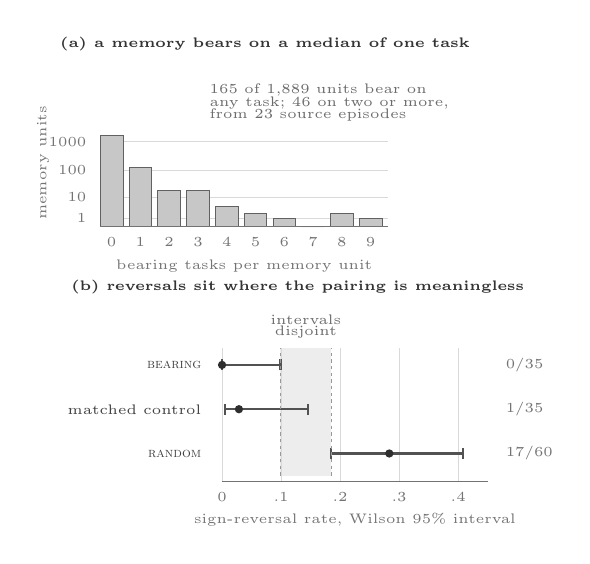
\begin{tikzpicture}[
  font=\scriptsize,
  bar/.style={draw=black!62, fill=black!22, line width=0.3pt},
  ax/.style={draw=black!55, line width=0.4pt},
  gl/.style={draw=black!15, line width=0.3pt},
  tk/.style={font=\tiny, text=black!55},
  note/.style={font=\tiny, text=black!58, align=left},
  hd/.style={font=\tiny\bfseries, text=black!80},
  ci/.style={draw=black!68, line width=0.8pt},
  whisk/.style={draw=black!68, line width=0.8pt},
]
\def\bw{8.2pt}
% ================= PANEL A =================
\begin{scope}
  \foreach \h/\l in {\bearTickZero/1,\bearTickOne/10,\bearTickTwo/100,\bearTickThree/1000}{
    \draw[gl] (0,\h) -- (\bearAxisW,\h);
    \node[tk, left=1.5pt] at (0,\h) {\l};
  }
  \foreach \i/\h/\n in {0/\bearHZero/\bearNZero, 1/\bearHOne/\bearNOne,
                        2/\bearHTwo/\bearNTwo, 3/\bearHThree/\bearNThree,
                        4/\bearHFour/\bearNFour, 5/\bearHFive/\bearNFive,
                        6/\bearHSix/\bearNSix, 7/\bearHSeven/\bearNSeven,
                        8/\bearHEight/\bearNEight, 9/\bearHNine/\bearNNine}{
    \pgfmathsetmacro{\xx}{\i*10.4}
    \draw[bar] (\xx pt,0) rectangle ({\xx pt+\bw},\h);
    \node[tk, below=0.5pt] at ({\xx pt+0.5*\bw},0) {\i};
  }
  \draw[ax] (0,0) -- (\bearAxisW,0);
  \node[hd, anchor=south west] at (-18pt,60pt) {(a) a memory bears on a median of one task};
  \node[note, anchor=north west] at (36pt,55pt)
    {\bearAny\ of \bearUnits\ units bear on\\[-1.5pt]any task; \bearGeTwo\ on two or more,\\[-1.5pt]from \bearEpisodes\ source episodes};
  \node[tk, anchor=north] at (52pt,-8.5pt) {bearing tasks per memory unit};
  \node[tk, rotate=90, anchor=south] at (-15pt,23pt) {memory units};
\end{scope}
% ================= PANEL B =================
\begin{scope}[yshift=-86pt, xshift=44pt]
  \foreach \x/\l in {\flipTickZero/0, \flipTickOne/.1, \flipTickTwo/.2, \flipTickThree/.3, \flipTickFour/.4}{
    \draw[gl] (\x,-6pt) -- (\x,42pt);
    \node[tk, below=0.5pt] at (\x,-6pt) {\l};
  }
  \draw[ax] (0,-6pt) -- (\flipAxisW,-6pt);
  \foreach \y/\lo/\x/\hi/\nm/\k/\n in {
      36/\flipBearXLo/\flipBearX/\flipBearXHi/{\textsc{bearing}}/\flipBearK/\flipBearN,
      20/\flipCtrlXLo/\flipCtrlX/\flipCtrlXHi/{matched control}/\flipCtrlK/\flipCtrlN,
       4/\flipRandXLo/\flipRandX/\flipRandXHi/{\textsc{random}}/\flipRandK/\flipRandN}{
    \draw[ci] (\lo,\y pt) -- (\hi,\y pt);
    \draw[whisk] (\lo,{\y pt-2pt}) -- (\lo,{\y pt+2pt});
    \draw[whisk] (\hi,{\y pt-2pt}) -- (\hi,{\y pt+2pt});
    \fill[black!82] (\x,\y pt) circle (1.5pt);
    \node[tk, text=black!75, anchor=east] at (-4pt,\y pt) {\nm};
    \node[tk, anchor=west] at ({\flipAxisW+3pt},\y pt) {\k/\n};
  }
  \node[hd, anchor=south west] at (-58pt,58pt) {(b) reversals sit where the pairing is meaningless};
  % The claim panel (b) exists to make legible: BEARING's Wilson UPPER bound
  % sits below RANDOM's Wilson LOWER bound, so the intervals do not overlap.
  % Shaded band spans exactly that gap; both edges come from figdata.tex.
  \begin{scope}[on background layer]
    \fill[black!7] (\flipBearXHi,-4pt) rectangle (\flipRandXLo,42pt);
  \end{scope}
  \draw[draw=black!40, line width=0.3pt, dash pattern=on 1.2pt off 1.2pt]
    (\flipBearXHi,-4pt) -- (\flipBearXHi,42pt);
  \draw[draw=black!40, line width=0.3pt, dash pattern=on 1.2pt off 1.2pt]
    (\flipRandXLo,-4pt) -- (\flipRandXLo,42pt);
  \node[tk, text=black!58, anchor=south, font=\tiny, align=center] at
    ($(\flipBearXHi,42pt)!0.5!(\flipRandXLo,42pt)$) {intervals\\[-2pt]disjoint};
  \node[tk, anchor=north] at (48pt,-14pt) {sign-reversal rate, Wilson 95\% interval};
\end{scope}
\end{tikzpicture}
\caption{The two structural facts behind the result. \textbf{(a)} Over all
$\bearUnits$ naturally occurring memory units screened against the
$\bearDetTasks$ deterministically scored discriminative tasks, the number of
future tasks a memory bears on is concentrated at one; the count axis is
logarithmic and a zero count is drawn as no bar. This caps the denominator of
any reversal rate at the $\bearGeTwo$ units with two or more bearing tasks,
on only $\bearEpisodes$ source episodes. \textbf{(b)} Sign-reversal rate by
stratum, Wilson $95\%$ intervals and eligible denominators.
\textsc{bearing}'s interval lies entirely below \textsc{random}'s: reversals
concentrate where memories are paired with unrelated tasks. These rates are
descriptive; we draw no inference about the memory\,$\times$\,task
interaction from them (Section~\ref{sec:metrics}).}
\label{fig:bearing}
\end{figure}

\subsection{Memory utility is sparse across future tasks}
\label{sec:scarcity}
%%% Source: docs/BEARING_SCARCITY.md; data/manifests/lmev2_leakage_small.jsonl.
%%% Re-derived by the coordinating author from the manifest, not read off a report.
Screening all 1{,}889 naturally occurring memory units against the 295
deterministically scored LongMemEval-V2 questions, with a content-only
detector that must single a memory out of its same-domain pool, yields 76
discriminative tasks, 75 of them deterministically scored. Over those 75 ---
the basis the executed design uses throughout --- 165 memories have at least
one bearing task across 266 memory--task edges, heavily concentrated at one:
119 bear on exactly one task, 18 on two, 18 on three, with a tail reaching
nine (Figure~\ref{fig:bearing}, left). \emph{A naturally occurring memory in
this corpus bears on a median of one future task out of hundreds.}
%%% BASIS, stated because the two differ and mixing them is a real error we made:
%%% over the 76 discriminative tasks the edge count is 267 and the histogram is
%%% {1:119, 2:18, 3:17, 4:5, ...}; over the 75 DETERMINISTIC ones it is 266 and
%%% {1:119, 2:18, 3:18, 4:4, ...}. The executed design (k1_screened_design.json:
%%% n_discriminative_tasks=75, n_bearing_edges_total=266) and scripts/audit_claims.py
%%% both use the 75-task basis, so the manuscript does too. An earlier draft of this
%%% paragraph quoted 267 edges and "17 on three" from the 76-task basis while
%%% describing the 75-task one. scripts/make_figures.py now pins this.

A sign change needs one memory with two bearing cells of opposite sign, so
any flip rate's denominator is the 46 memories with two or more bearing tasks
--- and those sit on only 23 distinct source trajectories, so they are not 46
independent draws. We report unit-level and episode-clustered denominators
throughout and let the clustered interval govern.

\paragraph{Indiscriminate pairing is mostly structural zeros.}
\label{sec:dilution}
%%% Source: results/ledgers/repro/{pilot,official}_cells_slim.jsonl (tracked);
%%% full artifacts' sha256 in results/ledgers/repro/MANIFEST.json.
Pairing each memory with same-domain questions chosen for question-type
spread, without requiring that the memory bear on the question, produces
cells in which the reader fails \emph{both} with and without the memory: a
structural zero whether or not the memory is useful. We measure this at
$376/479$ and $402/480$ in two prompt arms --- about $80\%$ of cells --- so a
null there is uninformative rather than negative.


\subsection{Screening makes the memory effect measurable}
\label{sec:screened}
%%% Source: results/deltau_screened/cells.jsonl (5,198 calls, 0 errors).
%%% All figures re-derived by the coordinating author from the row file; the
%%% stratum is carried natively on all 2,599 rows AND recoverable by design
%%% join, and the two routes agree exactly.
We repeat the measurement with the memory--task pairing screened by the
content-only criterion, against a matched control and the unscreened design;
all three strata contain the \emph{identical} 60 memories, so the contrast is
paired within memory.

\begin{table}[t]
\centering\small
\caption{Screened run. Both-arms-fail is the fraction of cells in which the
reader fails with \emph{and} without the memory; such cells cannot exhibit a
memory effect. The criterion for ``materially reduced'' --- the \textsc{bearing}
Wilson upper bound below the comparator's point estimate --- was fixed in code
before these numbers existed.}
\label{tab:screened}
\begin{tabular}{lrrr}
\toprule
stratum & both-arms-fail & 95\% Wilson & mean $\Delta U$ \\
\midrule
%%% The mean-dU column now reads the GENERATED macros, which are the same
%%% values Figure 4(b) plotted. They had been typed here and generated there
%%% -- the exact duplication (one display hand-entered, one generated) that
%%% this manuscript already removed once for the sign-reversal table. The
%%% figure's panel (b) is dropped and the column kept, since the table also
%%% carries both-arms-fail and the Wilson bounds the panel could not show.
\textsc{bearing}      & \textbf{0.5252} & [0.4426, \textbf{0.6064}] & \textbf{\stratBearV} \\
matched control       & 0.7877 & [0.7144, 0.8462] & \stratCtrlV \\
random (unscreened)   & 0.7007 & [0.6695, 0.7302] & \stratRandV \\
\bottomrule
\end{tabular}
\end{table}

%%% ============ FIGURE: THE SPARSITY MAP =================================
%%% THE PAPER'S CENTRAL CLAIM HAD NO FIGURE. "A global memory score is
%%% insufficient because utility is sparse across future tasks" was carried
%%% only by table rows. This draws the cell-level evidence: one square per
%%% MEASURED cell, all 1,157 of them.
%%%
%%% EVERY COORDINATE comes from \spPos / \spNeg / \spZero in figdata.tex,
%%% emitted by scripts/make_figures.py::sparsity_map(). TikZ iterates the
%%% lists and computes nothing; there is no arithmetic on a measurement here.
%%%
%%% FOUR DESIGN CONSTRAINTS, each forced by a checked property of the data:
%%%   1. dU is EXACTLY three-valued (-1/0/+1) because the reward is binary
%%%      and both replicates agree on every one of the 1,157 cells. A
%%%      continuous colour ramp would imply precision the data lacks, so
%%%      three discrete marks. The generator FAILS if a fourth level appears.
%%%   2. UNMEASURED SLOTS ARE NOT DRAWN. Rows are ragged (max 9/9/15 cells
%%%      per memory). Padding to a rectangle makes the eye read marks per
%%%      AREA -- 9.3% BEARING vs 9.1% RANDOM, indistinguishable and the
%%%      opposite of the finding. Per DRAWN square it is 36.0% vs 9.4%.
%%%      make_figures.py asserts BOTH readings and fails if they converge.
%%%   3. A MEASURED ZERO IS DRAWN (light square); an ABSENT cell is drawn as
%%%      nothing. An absence rendered as a value is this project's named
%%%      defect shape, and a measured zero is a real finding.
%%%   4. ROWS ARE SORTED by BEARING positive count, which the caption
%%%      discloses. The sort cannot manufacture the claim: the stratum
%%%      contrast is also given as positive RATES with Wilson intervals,
%%%      and the generator fails if BEARING's interval stops sitting
%%%      entirely above RANDOM's.
\begin{figure}[t]
\centering
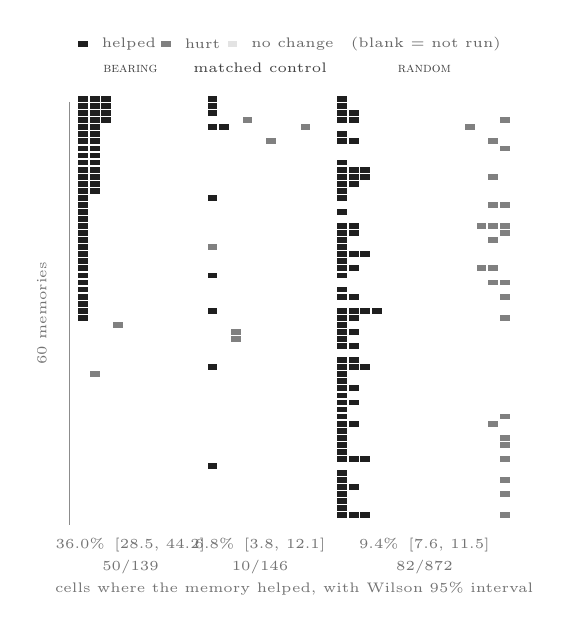
\begin{tikzpicture}[
  font=\scriptsize,
  tk/.style={font=\tiny, text=black!55},
  hd/.style={font=\tiny\bfseries, text=black!80},
  lg/.style={font=\tiny, text=black!60},
  br/.style={draw=black!45, line width=0.35pt},
]
\def\cw{3.5pt}\def\ch{2.1pt}
%% ---- the cells. Order matters: zeros first, so a non-zero mark is never
%% painted over by a neighbouring zero.
\foreach \x/\y in \spZero
  { \fill[black!11] (\x pt,\y pt) rectangle +(\cw,\ch); }
\foreach \x/\y in \spNeg
  { \fill[black!50] (\x pt,\y pt) rectangle +(\cw,\ch); }
\foreach \x/\y in \spPos
  { \fill[black!88] (\x pt,\y pt) rectangle +(\cw,\ch); }
%% ---- stratum headers and the per-block positive rate
\foreach \mi/\nm/\rt/\lo/\hi in {%
    \spBearMid/{\textsc{bearing}}/\spBearRate/\spBearLo/\spBearHi,
    \spCtrlMid/{matched control}/\spCtrlRate/\spCtrlLo/\spCtrlHi,
    \spRandMid/{\textsc{random}}/\spRandRate/\spRandLo/\spRandHi}{
  \node[tk, text=black!75, anchor=south] at (\mi,7pt) {\nm};
  \node[tk, anchor=north] at (\mi,{-\spTotH-1pt})
    {\rt\%\ \,{\tiny[\lo, \hi]}};
}
\node[tk, anchor=north] at (\spBearMid,{-\spTotH-9pt}) {\spBearPos/\spBearN};
\node[tk, anchor=north] at (\spCtrlMid,{-\spTotH-9pt}) {\spCtrlPos/\spCtrlN};
\node[tk, anchor=north] at (\spRandMid,{-\spTotH-9pt}) {\spRandPos/\spRandN};
\node[tk, anchor=north] at (78pt,{-\spTotH-17pt})
  {cells where the memory helped, with Wilson 95\% interval};
%% ---- the memory axis
\draw[br] (-3pt,0pt) -- (-3pt,{-\spTotH});
\node[tk, rotate=90, anchor=south] at (-8pt,{-0.5*\spTotH})
  {\spMems\ memories};
%% ---- legend, raised clear of the stratum headers
\fill[black!88] (0pt,20pt) rectangle +(\cw,\ch);
\node[lg, anchor=west] at (5pt,21pt) {helped};
\fill[black!50] (30pt,20pt) rectangle +(\cw,\ch);
\node[lg, anchor=west] at (35pt,21pt) {hurt};
\fill[black!11] (54pt,20pt) rectangle +(\cw,\ch);
\node[lg, anchor=west] at (59pt,21pt) {no change};
\node[lg, anchor=west] at (95pt,21pt) {(blank $=$ not run)};
\end{tikzpicture}
\caption{\textbf{Utility is sparse over future tasks, and the sparsity is
structured.} One square per \emph{measured} cell --- all $\spCells$ of them,
$\spMems$ memories $\times$ their own future tasks, one representation and
one frozen reader. $\Delta U$ takes exactly three values here, so the marks
are discrete rather than shaded. Only $\spNonzero$ cells move at all:
$\spZeroPct\%$ of measured cells are an exact zero, which is the quantity a
single global memory score has to summarise. The three blocks are the same $\spMems$
memories against bearing, matched-control and unscreened tasks, so the
comparison is paired within memory. Rows are ordered by \textsc{bearing}
count; that arranges the rows but cannot create the block contrast, which is
$\spBearRate\%$ against $\spRandRate\%$ with disjoint Wilson intervals. A row's squares are that memory's own tasks in its
own order, so a \emph{column is not a task}: the blocks span $\spBearTasks$,
$\spCtrlTasks$ and $\spRandTasks$ distinct tasks against widths of 9, 9 and
15. Unrun cells are blank rather than padded --- the rows are ragged, and
padding them would spread the same marks over more area and collapse the
contrast to about $1\times$.}
\label{fig:sparsity}
\end{figure}

The pre-committed rule returns that the screen bought measurement capacity
(Table~\ref{tab:screened}). Figure~\ref{fig:sparsity} shows the same
measurement one cell at a time: $\spZeroPct\%$ of the $\spCells$ measured
cells are an exact zero, and the cells that are not concentrate in the
\textsc{bearing} block --- $\spBearRate\%$ of bearing cells against
$\spRandRate\%$ unscreened, on the same $\spMems$ memories. This is what a
single global score per memory has to stand in for. The matched control
reproduces the prior
unscreened design ($0.7850$) almost exactly: the objection that screening
merely selected easier tasks predicts an easier control, and it is not
easier; combined with the within-memory pairing, the gap is hard to attribute
to anything but whether the memory bears on the task.

\paragraph{The paired effect.}
Each memory contributes one difference, its mean $\Delta U$ on bearing cells
minus its mean on control cells. Over all 60 memories the mean is $+0.3349$;
over the 35 with a non-zero contribution it is $+0.5740$. The bootstrap over
memories gives $[+0.2085, +0.4606]$ and the episode-clustered bootstrap,
which governs, gives $[+0.1974, +0.4736]$; both exclude zero. We report all
three because the all-memory mean is diluted by memories failing in both
arms, while the contributors-only mean conditions on an outcome.


\paragraph{The bottleneck is the pairing, not the reader.}
\label{sec:notreader}
%%% Source: results/j2_escalation/needle_summary.json (22/22, and 0/17 negative
%%% control); docs/PAIRING_VERDICT.md.
Planting a per-cell unique code inside the target memory, in the real
$\sim$27k-token context, and asking for it back recovers it in $22/22$ cells
under the base reader and $0/17$ when nothing is planted; two larger models
also recover $22/22$ and solve no cell the base reader missed. The reader can
locate and use memory content at full context length, so low accuracy on
unscreened cells is not a capability ceiling.

\paragraph{The same contrast in the two earlier, unscreened arms.}
\label{sec:effect}
%%% Source: coordinating author's re-derivation from the two slim artifacts and
%%% results/ledgers/j1b_discriminative_oracle_thr8.json (sweep key
%%% max_pool_hits<=8, NOT the file's <=5 default).
On bearing cells --- a subgroup defined by content, with no outcome entering
its definition --- mean $\Delta U$ is $+0.0909$ and $+0.1818$ in the two
arms, against $-0.0066$ and $-0.0153$ elsewhere. Pooled, $+0.1364$ versus
$-0.0109$: a difference of $+0.1473$, permutation $p = 0.0029$ over
20{,}000 shuffles. Accuracy is monotone in how discriminatively the memory
matches the task: $0.1429 \rightarrow 0.4545 \rightarrow 0.5000$.

\paragraph{Position is a confound, and we hold it fixed.}
\label{sec:position}
%%% Source: docs/POSITION_EFFECT.md. PROVISIONAL: n=12.
Holding the memory, question, filler, model, decoding and seed fixed and
varying \emph{only} the position of the target memory changes the answer in
$8$ of $12$ cells. The with-memory arm necessarily holds one more item, so
some rule must place it, and that rule is not neutral: a comparison not
controlling position measures position together with presence. Provisional at
$n=12$; we hold position fixed across replicates, vary it across cells, and
record it on every row --- which is also what makes
Section~\ref{sec:readertransfer} a reader comparison and not a position one.

%%% ===================== FIGURE 3: similarity vs the content screen ============
%%% ALL VALUES GENERATED into figdata.tex by scripts/make_figures.py from
%%% results/ledgers/repro/screened_cells_slim.jsonl. Nothing typed by hand.
%%%
%%% WHY PANEL (a) CARRIES TWO SERIES. BEARING cells concentrate in the high
%%% similarity bins -- 54 of 139 in the top sextile against 5 in the bottom --
%%% so the pooled trend is PARTLY the content screen showing through, and
%%% plotting it alone would credit the embedding with the screen's work. The
%%% unscreened-only series is the same axis with no bearing cells in it. The
%%% generator asserts that concentration, so the confound cannot silently go
%%% away without this comment going stale loudly.
\begin{figure}[t]
\centering
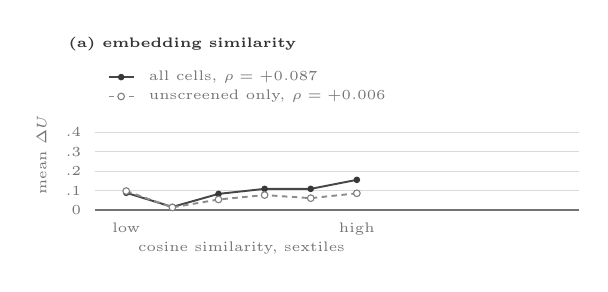
\begin{tikzpicture}[
  font=\scriptsize,
  ax/.style={draw=black!55, line width=0.4pt},
  gl/.style={draw=black!15, line width=0.3pt},
  tk/.style={font=\tiny, text=black!55},
  note/.style={font=\tiny, text=black!58, align=left},
  hd/.style={font=\tiny\bfseries, text=black!80},
  simline/.style={draw=black!72, line width=0.7pt},
  randline/.style={draw=black!45, line width=0.7pt, dash pattern=on 2pt off 1.6pt},
  stratbar/.style={draw=black!68, line width=0.35pt},
]
% ---- y axis (shared) ----
\foreach \y/\l in {\simTickZero/0, \simTickOne/.1, \simTickTwo/.2, \simTickThree/.3, \simTickFour/.4}{
  \draw[gl] (-3pt,\y) -- (172pt,\y);
  \node[tk, left=1.5pt] at (-3pt,\y) {\l};
}
\draw[ax] (-3pt,0) -- (172pt,0);
\node[tk, rotate=90, anchor=south] at (-17pt,20pt) {mean $\Delta U$};
% ================= LEFT: similarity sextiles =================
\draw[simline]
  (\simXZero,\simPooledYZero) -- (\simXOne,\simPooledYOne) -- (\simXTwo,\simPooledYTwo)
  -- (\simXThree,\simPooledYThree) -- (\simXFour,\simPooledYFour) -- (\simXFive,\simPooledYFive);
\draw[randline]
  (\simXZero,\simRandYZero) -- (\simXOne,\simRandYOne) -- (\simXTwo,\simRandYTwo)
  -- (\simXThree,\simRandYThree) -- (\simXFour,\simRandYFour) -- (\simXFive,\simRandYFive);
\foreach \x/\y in {\simXZero/\simPooledYZero, \simXOne/\simPooledYOne, \simXTwo/\simPooledYTwo,
                   \simXThree/\simPooledYThree, \simXFour/\simPooledYFour, \simXFive/\simPooledYFive}
  \fill[black!78] (\x,\y) circle (1.2pt);
\foreach \x/\y in {\simXZero/\simRandYZero, \simXOne/\simRandYOne, \simXTwo/\simRandYTwo,
                   \simXThree/\simRandYThree, \simXFour/\simRandYFour, \simXFive/\simRandYFive}
  \draw[draw=black!50, fill=white, line width=0.4pt] (\x,\y) circle (1.2pt);
\node[tk, anchor=north] at (\simXZero,-1pt) {low};
\node[tk, anchor=north] at (\simXFive,-1pt) {high};
\node[tk, anchor=north] at (50pt,-8pt) {cosine similarity, sextiles};
\node[hd, anchor=south west] at (-16pt,54pt) {(a) embedding similarity};
% inline legend, placed in the empty upper-left where no series runs
\draw[simline] (2pt,48pt) -- (11pt,48pt); \fill[black!78] (6.5pt,48pt) circle (1.2pt);
\node[tk, anchor=west] at (13pt,48pt) {all cells, $\rho=\simRhoAll$};
\draw[randline] (2pt,41pt) -- (11pt,41pt);
\draw[draw=black!50, fill=white, line width=0.4pt] (6.5pt,41pt) circle (1.2pt);
\node[tk, anchor=west] at (13pt,41pt) {unscreened only, $\rho=\simRhoRand$};
\end{tikzpicture}
\caption{Similarity does not locate a useful memory. Mean $\Delta U$ by
equal-count sextile of memory--task cosine similarity is nearly flat ---
Spearman $\rho=\simRhoAll$ over all $\simCells$ cells --- against the
content-based bearing criterion, which uses no embedding at all and separates
$\stratBearV$ from $\stratCtrlV$ (Table~\ref{tab:screened}). Because
\textsc{bearing} cells concentrate in the upper sextiles the pooled series
partly reflects the content screen rather than the embedding; the
unscreened-only series isolates similarity and is flatter still
($\rho=\simRhoRand$). Similarity is computed on a truncated prefix for most
memories, which attenuates any relationship toward zero, so this is a lower
bound on what this embedding could do.}
\label{fig:similarity}
\end{figure}

\subsection{Semantic similarity poorly locates utility}
\label{sec:similarity}
Cosine similarity between the memory and the task, under the pinned embedding
model, is nearly uninformative about $\Delta U$, reaching Spearman
$\rho = +0.164$ even within \textsc{bearing}, while the content-based
criterion separates the strata (Figure~\ref{fig:similarity}). What makes a
memory useful is visible to a detector asking what it \emph{contains} and
largely invisible to one asking what it resembles --- on one embedding model
and corpus, with $96.6\%$ of the executed cells' similarities computed from a
truncated prefix at the adopted embedding budget, which attenuates the
relationship toward zero.



%%% ===================== FIGURE 4: the utility--efficiency frontier ===========
%%% EVERY NUMBER GENERATED, NOT TYPED. All coordinates, endpoints, token counts
%%% and ratios come from %%% GENERATED by scripts/make_figures.py in the code repository.
%%% DO NOT EDIT BY HAND, and do not edit a value here to make a
%%% figure look right -- regenerate. Every value is recomputed from
%%% a tracked artifact and cross-checked against the audited value;
%%% the generator exits non-zero on any disagreement, and a planted
%%% sign flip in one BEARING cell is verified to make it fail.
%%% Sources: data/manifests/lmev2_leakage_small.jsonl
%%%          results/ledgers/repro/screened_cells_slim.jsonl
%%%          results/ledgers/k1_screened_design.json (basis pin)

%% --- sparsity map (fig 1b): one square per MEASURED cell ---
%% The paper's central claim, drawn at cell level. dU is exactly
%% three-valued (-1/0/+1) and the generator FAILS if a fourth
%% level appears. Unmeasured slots are drawn as NOTHING: the
%% rows are ragged, and padding them to a rectangle collapses
%% the BEARING/RANDOM contrast from 3.83x to 1.02x -- both
%% readings are asserted so a padded redraw cannot pass.
\def\spPos{0.00/0.00,4.20/0.00,8.40/0.00,46.80/0.00,93.60/0.00,0.00/-2.55,4.20/-2.55,8.40/-2.55,46.80/-2.55,93.60/-2.55,0.00/-5.10,4.20/-5.10,8.40/-5.10,46.80/-5.10,93.60/-5.10,97.80/-5.10,0.00/-7.65,4.20/-7.65,8.40/-7.65,93.60/-7.65,97.80/-7.65,0.00/-10.20,4.20/-10.20,46.80/-10.20,51.00/-10.20,0.00/-12.75,4.20/-12.75,93.60/-12.75,0.00/-15.30,4.20/-15.30,93.60/-15.30,97.80/-15.30,0.00/-17.85,4.20/-17.85,0.00/-20.40,4.20/-20.40,0.00/-22.95,4.20/-22.95,93.60/-22.95,0.00/-25.50,4.20/-25.50,93.60/-25.50,97.80/-25.50,102.00/-25.50,0.00/-28.05,4.20/-28.05,93.60/-28.05,97.80/-28.05,102.00/-28.05,0.00/-30.60,4.20/-30.60,93.60/-30.60,97.80/-30.60,0.00/-33.15,4.20/-33.15,93.60/-33.15,0.00/-35.70,46.80/-35.70,93.60/-35.70,0.00/-38.25,0.00/-40.80,93.60/-40.80,0.00/-43.35,0.00/-45.90,93.60/-45.90,97.80/-45.90,0.00/-48.45,93.60/-48.45,97.80/-48.45,0.00/-51.00,93.60/-51.00,0.00/-53.55,93.60/-53.55,0.00/-56.10,93.60/-56.10,97.80/-56.10,102.00/-56.10,0.00/-58.65,93.60/-58.65,0.00/-61.20,93.60/-61.20,97.80/-61.20,0.00/-63.75,46.80/-63.75,93.60/-63.75,0.00/-66.30,0.00/-68.85,93.60/-68.85,0.00/-71.40,93.60/-71.40,97.80/-71.40,0.00/-73.95,0.00/-76.50,46.80/-76.50,93.60/-76.50,97.80/-76.50,102.00/-76.50,106.20/-76.50,0.00/-79.05,93.60/-79.05,97.80/-79.05,93.60/-81.60,93.60/-84.15,97.80/-84.15,93.60/-86.70,93.60/-89.25,97.80/-89.25,93.60/-94.35,97.80/-94.35,46.80/-96.90,93.60/-96.90,97.80/-96.90,102.00/-96.90,93.60/-99.45,93.60/-102.00,93.60/-104.55,97.80/-104.55,93.60/-107.10,93.60/-109.65,97.80/-109.65,93.60/-112.20,93.60/-114.75,93.60/-117.30,97.80/-117.30,93.60/-119.85,93.60/-122.40,93.60/-124.95,93.60/-127.50,93.60/-130.05,97.80/-130.05,102.00/-130.05,46.80/-132.60,93.60/-135.15,93.60/-137.70,93.60/-140.25,97.80/-140.25,93.60/-142.80,93.60/-145.35,93.60/-147.90,93.60/-150.45,97.80/-150.45,102.00/-150.45}
\def\spNeg{59.40/-7.65,152.40/-7.65,80.40/-10.20,139.80/-10.20,67.80/-15.30,148.20/-15.30,152.40/-17.85,148.20/-28.05,148.20/-38.25,152.40/-38.25,144.00/-45.90,148.20/-45.90,152.40/-45.90,152.40/-48.45,148.20/-51.00,46.80/-53.55,144.00/-61.20,148.20/-61.20,148.20/-66.30,152.40/-66.30,152.40/-71.40,152.40/-79.05,12.60/-81.60,55.20/-84.15,55.20/-86.70,4.20/-99.45,152.40/-114.75,148.20/-117.30,152.40/-122.40,152.40/-124.95,152.40/-130.05,152.40/-137.70,152.40/-142.80,152.40/-150.45}
\def\spZero{12.60/0.00,16.80/0.00,21.00/0.00,25.20/0.00,29.40/0.00,33.60/0.00,51.00/0.00,55.20/0.00,59.40/0.00,63.60/0.00,67.80/0.00,72.00/0.00,76.20/0.00,80.40/0.00,97.80/0.00,102.00/0.00,106.20/0.00,110.40/0.00,114.60/0.00,118.80/0.00,123.00/0.00,127.20/0.00,131.40/0.00,135.60/0.00,139.80/0.00,144.00/0.00,148.20/0.00,12.60/-2.55,16.80/-2.55,21.00/-2.55,25.20/-2.55,29.40/-2.55,51.00/-2.55,55.20/-2.55,59.40/-2.55,63.60/-2.55,67.80/-2.55,72.00/-2.55,76.20/-2.55,80.40/-2.55,97.80/-2.55,102.00/-2.55,106.20/-2.55,110.40/-2.55,114.60/-2.55,118.80/-2.55,123.00/-2.55,127.20/-2.55,131.40/-2.55,135.60/-2.55,139.80/-2.55,12.60/-5.10,51.00/-5.10,55.20/-5.10,59.40/-5.10,102.00/-5.10,106.20/-5.10,110.40/-5.10,114.60/-5.10,118.80/-5.10,123.00/-5.10,127.20/-5.10,131.40/-5.10,135.60/-5.10,139.80/-5.10,144.00/-5.10,148.20/-5.10,152.40/-5.10,46.80/-7.65,51.00/-7.65,55.20/-7.65,102.00/-7.65,106.20/-7.65,110.40/-7.65,114.60/-7.65,118.80/-7.65,123.00/-7.65,127.20/-7.65,131.40/-7.65,135.60/-7.65,139.80/-7.65,144.00/-7.65,148.20/-7.65,8.40/-10.20,12.60/-10.20,16.80/-10.20,21.00/-10.20,25.20/-10.20,29.40/-10.20,55.20/-10.20,59.40/-10.20,63.60/-10.20,67.80/-10.20,72.00/-10.20,76.20/-10.20,93.60/-10.20,97.80/-10.20,102.00/-10.20,106.20/-10.20,110.40/-10.20,114.60/-10.20,118.80/-10.20,123.00/-10.20,127.20/-10.20,131.40/-10.20,135.60/-10.20,8.40/-12.75,12.60/-12.75,16.80/-12.75,46.80/-12.75,51.00/-12.75,55.20/-12.75,59.40/-12.75,63.60/-12.75,67.80/-12.75,97.80/-12.75,102.00/-12.75,106.20/-12.75,110.40/-12.75,114.60/-12.75,118.80/-12.75,123.00/-12.75,127.20/-12.75,131.40/-12.75,135.60/-12.75,139.80/-12.75,144.00/-12.75,148.20/-12.75,8.40/-15.30,12.60/-15.30,16.80/-15.30,46.80/-15.30,51.00/-15.30,55.20/-15.30,59.40/-15.30,63.60/-15.30,102.00/-15.30,106.20/-15.30,110.40/-15.30,114.60/-15.30,118.80/-15.30,123.00/-15.30,127.20/-15.30,131.40/-15.30,135.60/-15.30,139.80/-15.30,144.00/-15.30,8.40/-17.85,46.80/-17.85,51.00/-17.85,55.20/-17.85,59.40/-17.85,93.60/-17.85,97.80/-17.85,102.00/-17.85,106.20/-17.85,110.40/-17.85,114.60/-17.85,118.80/-17.85,123.00/-17.85,127.20/-17.85,131.40/-17.85,135.60/-17.85,139.80/-17.85,144.00/-17.85,148.20/-17.85,8.40/-20.40,46.80/-20.40,51.00/-20.40,55.20/-20.40,93.60/-20.40,97.80/-20.40,102.00/-20.40,106.20/-20.40,110.40/-20.40,114.60/-20.40,118.80/-20.40,123.00/-20.40,127.20/-20.40,131.40/-20.40,135.60/-20.40,139.80/-20.40,144.00/-20.40,148.20/-20.40,152.40/-20.40,8.40/-22.95,46.80/-22.95,51.00/-22.95,55.20/-22.95,97.80/-22.95,102.00/-22.95,106.20/-22.95,110.40/-22.95,114.60/-22.95,118.80/-22.95,123.00/-22.95,127.20/-22.95,131.40/-22.95,135.60/-22.95,139.80/-22.95,144.00/-22.95,148.20/-22.95,152.40/-22.95,8.40/-25.50,46.80/-25.50,51.00/-25.50,55.20/-25.50,106.20/-25.50,110.40/-25.50,114.60/-25.50,118.80/-25.50,123.00/-25.50,127.20/-25.50,131.40/-25.50,135.60/-25.50,139.80/-25.50,144.00/-25.50,148.20/-25.50,8.40/-28.05,46.80/-28.05,51.00/-28.05,55.20/-28.05,106.20/-28.05,110.40/-28.05,114.60/-28.05,118.80/-28.05,123.00/-28.05,127.20/-28.05,131.40/-28.05,135.60/-28.05,139.80/-28.05,144.00/-28.05,46.80/-30.60,51.00/-30.60,102.00/-30.60,106.20/-30.60,110.40/-30.60,114.60/-30.60,118.80/-30.60,123.00/-30.60,127.20/-30.60,131.40/-30.60,135.60/-30.60,139.80/-30.60,144.00/-30.60,148.20/-30.60,152.40/-30.60,46.80/-33.15,51.00/-33.15,97.80/-33.15,102.00/-33.15,106.20/-33.15,110.40/-33.15,114.60/-33.15,118.80/-33.15,123.00/-33.15,127.20/-33.15,131.40/-33.15,135.60/-33.15,139.80/-33.15,144.00/-33.15,148.20/-33.15,4.20/-35.70,8.40/-35.70,12.60/-35.70,51.00/-35.70,55.20/-35.70,59.40/-35.70,97.80/-35.70,102.00/-35.70,106.20/-35.70,110.40/-35.70,114.60/-35.70,118.80/-35.70,123.00/-35.70,127.20/-35.70,131.40/-35.70,135.60/-35.70,139.80/-35.70,144.00/-35.70,4.20/-38.25,8.40/-38.25,46.80/-38.25,51.00/-38.25,55.20/-38.25,59.40/-38.25,93.60/-38.25,97.80/-38.25,102.00/-38.25,106.20/-38.25,110.40/-38.25,114.60/-38.25,118.80/-38.25,123.00/-38.25,127.20/-38.25,131.40/-38.25,135.60/-38.25,139.80/-38.25,144.00/-38.25,4.20/-40.80,46.80/-40.80,51.00/-40.80,97.80/-40.80,102.00/-40.80,106.20/-40.80,110.40/-40.80,114.60/-40.80,118.80/-40.80,123.00/-40.80,127.20/-40.80,131.40/-40.80,135.60/-40.80,139.80/-40.80,144.00/-40.80,148.20/-40.80,4.20/-43.35,46.80/-43.35,51.00/-43.35,93.60/-43.35,97.80/-43.35,102.00/-43.35,106.20/-43.35,110.40/-43.35,114.60/-43.35,118.80/-43.35,123.00/-43.35,127.20/-43.35,131.40/-43.35,135.60/-43.35,139.80/-43.35,144.00/-43.35,148.20/-43.35,4.20/-45.90,46.80/-45.90,51.00/-45.90,102.00/-45.90,106.20/-45.90,110.40/-45.90,114.60/-45.90,118.80/-45.90,123.00/-45.90,127.20/-45.90,131.40/-45.90,135.60/-45.90,139.80/-45.90,4.20/-48.45,46.80/-48.45,51.00/-48.45,102.00/-48.45,106.20/-48.45,110.40/-48.45,114.60/-48.45,118.80/-48.45,123.00/-48.45,127.20/-48.45,131.40/-48.45,135.60/-48.45,139.80/-48.45,144.00/-48.45,148.20/-48.45,4.20/-51.00,46.80/-51.00,51.00/-51.00,97.80/-51.00,102.00/-51.00,106.20/-51.00,110.40/-51.00,114.60/-51.00,118.80/-51.00,123.00/-51.00,127.20/-51.00,131.40/-51.00,135.60/-51.00,139.80/-51.00,144.00/-51.00,97.80/-53.55,102.00/-53.55,106.20/-53.55,110.40/-53.55,114.60/-53.55,118.80/-53.55,123.00/-53.55,127.20/-53.55,131.40/-53.55,135.60/-53.55,139.80/-53.55,144.00/-53.55,148.20/-53.55,152.40/-53.55,46.80/-56.10,106.20/-56.10,110.40/-56.10,114.60/-56.10,118.80/-56.10,123.00/-56.10,127.20/-56.10,131.40/-56.10,135.60/-56.10,139.80/-56.10,144.00/-56.10,148.20/-56.10,152.40/-56.10,46.80/-58.65,97.80/-58.65,102.00/-58.65,106.20/-58.65,110.40/-58.65,114.60/-58.65,118.80/-58.65,123.00/-58.65,127.20/-58.65,131.40/-58.65,135.60/-58.65,139.80/-58.65,144.00/-58.65,148.20/-58.65,152.40/-58.65,46.80/-61.20,102.00/-61.20,106.20/-61.20,110.40/-61.20,114.60/-61.20,118.80/-61.20,123.00/-61.20,127.20/-61.20,131.40/-61.20,135.60/-61.20,139.80/-61.20,97.80/-63.75,102.00/-63.75,106.20/-63.75,110.40/-63.75,114.60/-63.75,118.80/-63.75,123.00/-63.75,127.20/-63.75,131.40/-63.75,135.60/-63.75,139.80/-63.75,144.00/-63.75,148.20/-63.75,46.80/-66.30,93.60/-66.30,97.80/-66.30,102.00/-66.30,106.20/-66.30,110.40/-66.30,114.60/-66.30,118.80/-66.30,123.00/-66.30,127.20/-66.30,131.40/-66.30,135.60/-66.30,139.80/-66.30,144.00/-66.30,46.80/-68.85,97.80/-68.85,102.00/-68.85,106.20/-68.85,110.40/-68.85,114.60/-68.85,118.80/-68.85,123.00/-68.85,127.20/-68.85,131.40/-68.85,135.60/-68.85,139.80/-68.85,144.00/-68.85,148.20/-68.85,152.40/-68.85,46.80/-71.40,102.00/-71.40,106.20/-71.40,110.40/-71.40,114.60/-71.40,118.80/-71.40,123.00/-71.40,127.20/-71.40,131.40/-71.40,135.60/-71.40,139.80/-71.40,144.00/-71.40,148.20/-71.40,46.80/-73.95,93.60/-73.95,97.80/-73.95,102.00/-73.95,106.20/-73.95,110.40/-73.95,114.60/-73.95,118.80/-73.95,123.00/-73.95,127.20/-73.95,131.40/-73.95,135.60/-73.95,139.80/-73.95,144.00/-73.95,148.20/-73.95,110.40/-76.50,114.60/-76.50,118.80/-76.50,123.00/-76.50,127.20/-76.50,131.40/-76.50,135.60/-76.50,139.80/-76.50,144.00/-76.50,148.20/-76.50,152.40/-76.50,46.80/-79.05,102.00/-79.05,106.20/-79.05,110.40/-79.05,114.60/-79.05,118.80/-79.05,123.00/-79.05,127.20/-79.05,131.40/-79.05,135.60/-79.05,139.80/-79.05,144.00/-79.05,148.20/-79.05,0.00/-81.60,4.20/-81.60,8.40/-81.60,46.80/-81.60,51.00/-81.60,55.20/-81.60,59.40/-81.60,97.80/-81.60,102.00/-81.60,106.20/-81.60,110.40/-81.60,114.60/-81.60,118.80/-81.60,123.00/-81.60,127.20/-81.60,131.40/-81.60,135.60/-81.60,139.80/-81.60,144.00/-81.60,148.20/-81.60,152.40/-81.60,0.00/-84.15,4.20/-84.15,8.40/-84.15,46.80/-84.15,51.00/-84.15,102.00/-84.15,106.20/-84.15,110.40/-84.15,114.60/-84.15,118.80/-84.15,123.00/-84.15,127.20/-84.15,131.40/-84.15,135.60/-84.15,139.80/-84.15,144.00/-84.15,148.20/-84.15,0.00/-86.70,4.20/-86.70,8.40/-86.70,46.80/-86.70,51.00/-86.70,97.80/-86.70,102.00/-86.70,106.20/-86.70,110.40/-86.70,114.60/-86.70,118.80/-86.70,123.00/-86.70,127.20/-86.70,131.40/-86.70,135.60/-86.70,139.80/-86.70,144.00/-86.70,148.20/-86.70,152.40/-86.70,0.00/-89.25,4.20/-89.25,8.40/-89.25,46.80/-89.25,51.00/-89.25,55.20/-89.25,102.00/-89.25,106.20/-89.25,110.40/-89.25,114.60/-89.25,118.80/-89.25,123.00/-89.25,127.20/-89.25,131.40/-89.25,135.60/-89.25,139.80/-89.25,144.00/-89.25,148.20/-89.25,0.00/-91.80,4.20/-91.80,8.40/-91.80,46.80/-91.80,51.00/-91.80,55.20/-91.80,93.60/-91.80,97.80/-91.80,102.00/-91.80,106.20/-91.80,110.40/-91.80,114.60/-91.80,118.80/-91.80,123.00/-91.80,127.20/-91.80,131.40/-91.80,135.60/-91.80,139.80/-91.80,144.00/-91.80,148.20/-91.80,152.40/-91.80,0.00/-94.35,4.20/-94.35,8.40/-94.35,46.80/-94.35,51.00/-94.35,55.20/-94.35,102.00/-94.35,106.20/-94.35,110.40/-94.35,114.60/-94.35,118.80/-94.35,123.00/-94.35,127.20/-94.35,131.40/-94.35,135.60/-94.35,139.80/-94.35,144.00/-94.35,148.20/-94.35,152.40/-94.35,0.00/-96.90,4.20/-96.90,8.40/-96.90,51.00/-96.90,55.20/-96.90,106.20/-96.90,110.40/-96.90,114.60/-96.90,118.80/-96.90,123.00/-96.90,127.20/-96.90,131.40/-96.90,135.60/-96.90,139.80/-96.90,144.00/-96.90,148.20/-96.90,0.00/-99.45,46.80/-99.45,51.00/-99.45,97.80/-99.45,102.00/-99.45,106.20/-99.45,110.40/-99.45,114.60/-99.45,118.80/-99.45,123.00/-99.45,127.20/-99.45,131.40/-99.45,135.60/-99.45,139.80/-99.45,144.00/-99.45,0.00/-102.00,4.20/-102.00,46.80/-102.00,51.00/-102.00,97.80/-102.00,102.00/-102.00,106.20/-102.00,110.40/-102.00,114.60/-102.00,118.80/-102.00,123.00/-102.00,127.20/-102.00,131.40/-102.00,135.60/-102.00,139.80/-102.00,144.00/-102.00,148.20/-102.00,152.40/-102.00,0.00/-104.55,4.20/-104.55,46.80/-104.55,51.00/-104.55,102.00/-104.55,106.20/-104.55,110.40/-104.55,114.60/-104.55,118.80/-104.55,123.00/-104.55,127.20/-104.55,131.40/-104.55,135.60/-104.55,139.80/-104.55,144.00/-104.55,148.20/-104.55,0.00/-107.10,4.20/-107.10,46.80/-107.10,51.00/-107.10,97.80/-107.10,102.00/-107.10,106.20/-107.10,110.40/-107.10,114.60/-107.10,118.80/-107.10,123.00/-107.10,127.20/-107.10,131.40/-107.10,135.60/-107.10,139.80/-107.10,144.00/-107.10,148.20/-107.10,0.00/-109.65,4.20/-109.65,46.80/-109.65,51.00/-109.65,102.00/-109.65,106.20/-109.65,110.40/-109.65,114.60/-109.65,118.80/-109.65,123.00/-109.65,127.20/-109.65,131.40/-109.65,135.60/-109.65,139.80/-109.65,144.00/-109.65,148.20/-109.65,152.40/-109.65,0.00/-112.20,4.20/-112.20,46.80/-112.20,51.00/-112.20,97.80/-112.20,102.00/-112.20,106.20/-112.20,110.40/-112.20,114.60/-112.20,118.80/-112.20,123.00/-112.20,127.20/-112.20,131.40/-112.20,135.60/-112.20,139.80/-112.20,144.00/-112.20,148.20/-112.20,152.40/-112.20,0.00/-114.75,4.20/-114.75,46.80/-114.75,51.00/-114.75,97.80/-114.75,102.00/-114.75,106.20/-114.75,110.40/-114.75,114.60/-114.75,118.80/-114.75,123.00/-114.75,127.20/-114.75,131.40/-114.75,135.60/-114.75,139.80/-114.75,144.00/-114.75,148.20/-114.75,0.00/-117.30,46.80/-117.30,102.00/-117.30,106.20/-117.30,110.40/-117.30,114.60/-117.30,118.80/-117.30,123.00/-117.30,127.20/-117.30,131.40/-117.30,135.60/-117.30,139.80/-117.30,144.00/-117.30,0.00/-119.85,46.80/-119.85,97.80/-119.85,102.00/-119.85,106.20/-119.85,110.40/-119.85,114.60/-119.85,118.80/-119.85,123.00/-119.85,127.20/-119.85,131.40/-119.85,135.60/-119.85,139.80/-119.85,144.00/-119.85,148.20/-119.85,152.40/-119.85,0.00/-122.40,46.80/-122.40,97.80/-122.40,102.00/-122.40,106.20/-122.40,110.40/-122.40,114.60/-122.40,118.80/-122.40,123.00/-122.40,127.20/-122.40,131.40/-122.40,135.60/-122.40,139.80/-122.40,144.00/-122.40,148.20/-122.40,0.00/-124.95,46.80/-124.95,97.80/-124.95,102.00/-124.95,106.20/-124.95,110.40/-124.95,114.60/-124.95,118.80/-124.95,123.00/-124.95,127.20/-124.95,131.40/-124.95,135.60/-124.95,139.80/-124.95,144.00/-124.95,148.20/-124.95,0.00/-127.50,46.80/-127.50,97.80/-127.50,102.00/-127.50,106.20/-127.50,110.40/-127.50,114.60/-127.50,118.80/-127.50,123.00/-127.50,127.20/-127.50,131.40/-127.50,135.60/-127.50,139.80/-127.50,144.00/-127.50,148.20/-127.50,152.40/-127.50,0.00/-130.05,46.80/-130.05,106.20/-130.05,110.40/-130.05,114.60/-130.05,118.80/-130.05,123.00/-130.05,127.20/-130.05,131.40/-130.05,135.60/-130.05,139.80/-130.05,144.00/-130.05,148.20/-130.05,0.00/-132.60,93.60/-132.60,97.80/-132.60,102.00/-132.60,106.20/-132.60,110.40/-132.60,114.60/-132.60,118.80/-132.60,123.00/-132.60,127.20/-132.60,131.40/-132.60,135.60/-132.60,139.80/-132.60,144.00/-132.60,148.20/-132.60,152.40/-132.60,0.00/-135.15,46.80/-135.15,97.80/-135.15,102.00/-135.15,106.20/-135.15,110.40/-135.15,114.60/-135.15,118.80/-135.15,123.00/-135.15,127.20/-135.15,131.40/-135.15,135.60/-135.15,139.80/-135.15,144.00/-135.15,148.20/-135.15,152.40/-135.15,0.00/-137.70,46.80/-137.70,97.80/-137.70,102.00/-137.70,106.20/-137.70,110.40/-137.70,114.60/-137.70,118.80/-137.70,123.00/-137.70,127.20/-137.70,131.40/-137.70,135.60/-137.70,139.80/-137.70,144.00/-137.70,148.20/-137.70,0.00/-140.25,46.80/-140.25,102.00/-140.25,106.20/-140.25,110.40/-140.25,114.60/-140.25,118.80/-140.25,123.00/-140.25,127.20/-140.25,131.40/-140.25,135.60/-140.25,139.80/-140.25,144.00/-140.25,148.20/-140.25,152.40/-140.25,0.00/-142.80,46.80/-142.80,97.80/-142.80,102.00/-142.80,106.20/-142.80,110.40/-142.80,114.60/-142.80,118.80/-142.80,123.00/-142.80,127.20/-142.80,131.40/-142.80,135.60/-142.80,139.80/-142.80,144.00/-142.80,148.20/-142.80,0.00/-145.35,46.80/-145.35,97.80/-145.35,102.00/-145.35,106.20/-145.35,110.40/-145.35,114.60/-145.35,118.80/-145.35,123.00/-145.35,127.20/-145.35,131.40/-145.35,135.60/-145.35,139.80/-145.35,144.00/-145.35,148.20/-145.35,152.40/-145.35,0.00/-147.90,46.80/-147.90,97.80/-147.90,102.00/-147.90,106.20/-147.90,110.40/-147.90,114.60/-147.90,118.80/-147.90,123.00/-147.90,127.20/-147.90,131.40/-147.90,135.60/-147.90,139.80/-147.90,144.00/-147.90,148.20/-147.90,152.40/-147.90,0.00/-150.45,46.80/-150.45,106.20/-150.45,110.40/-150.45,114.60/-150.45,118.80/-150.45,123.00/-150.45,127.20/-150.45,131.40/-150.45,135.60/-150.45,139.80/-150.45,144.00/-150.45,148.20/-150.45}
\def\spCW{4.20pt}
\def\spRH{2.55pt}
\def\spTotW{156.60pt}
\def\spTotH{153.00pt}
\def\spBearX{0.00pt}
\def\spBearW{37.80pt}
\def\spBearMid{18.90pt}
\def\spBearN{139}
\def\spBearPos{50}
\def\spBearNeg{2}
\def\spBearRate{36.0}
\def\spBearLo{28.5}
\def\spBearHi{44.2}
\def\spCtrlX{46.80pt}
\def\spCtrlW{37.80pt}
\def\spCtrlMid{65.70pt}
\def\spCtrlN{146}
\def\spCtrlPos{10}
\def\spCtrlNeg{6}
\def\spCtrlRate{6.8}
\def\spCtrlLo{3.8}
\def\spCtrlHi{12.1}
\def\spRandX{93.60pt}
\def\spRandW{63.00pt}
\def\spRandMid{125.10pt}
\def\spRandN{872}
\def\spRandPos{82}
\def\spRandNeg{26}
\def\spRandRate{9.4}
\def\spRandLo{7.6}
\def\spRandHi{11.5}
\def\spCells{1{,}157}
\def\spMems{60}
\def\spNonzero{176}
\def\spZeroPct{84.8}
\def\spDrawnRatio{3.8}
\def\spBearTasks{56}
\def\spBearHelps{32}
\def\spCtrlTasks{100}
\def\spCtrlHelps{9}
\def\spRandTasks{147}
\def\spRandHelps{51}

%% --- bearing breadth: counts, and log-scaled bar heights in pt ---
\def\bearNZero{1724}
\def\bearHZero{33.00pt}
\def\bearNOne{119}
\def\bearHOne{21.20pt}
\def\bearNTwo{18}
\def\bearHTwo{13.04pt}
\def\bearNThree{18}
\def\bearHThree{13.04pt}
\def\bearNFour{4}
\def\bearHFour{7.13pt}
\def\bearNFive{2}
\def\bearHFive{4.86pt}
\def\bearNSix{1}
\def\bearHSix{3.07pt}
\def\bearNSeven{0}
\def\bearHSeven{0.00pt}
\def\bearNEight{2}
\def\bearHEight{4.86pt}
\def\bearNNine{1}
\def\bearHNine{3.07pt}
\def\bearUnits{1{,}889}
\def\bearAny{165}
\def\bearGeTwo{46}
\def\bearEpisodes{23}
\def\bearDetTasks{75}
\def\bearTickZero{3.07pt}
\def\bearTickOne{10.62pt}
\def\bearTickTwo{20.43pt}
\def\bearTickThree{30.59pt}

%% --- sign reversal: rate and Wilson bounds, as x-offsets in pt ---
\def\flipBearN{35}
\def\flipBearK{0}
\def\flipBearRate{0.0000}
\def\flipBearX{0.00pt}
\def\flipBearXLo{0.00pt}
\def\flipBearXHi{21.10pt}
\def\flipCtrlN{35}
\def\flipCtrlK{1}
\def\flipCtrlRate{0.0286}
\def\flipCtrlX{6.10pt}
\def\flipCtrlXLo{1.08pt}
\def\flipCtrlXHi{31.00pt}
\def\flipRandN{60}
\def\flipRandK{17}
\def\flipRandRate{0.2833}
\def\flipRandX{60.44pt}
\def\flipRandXLo{39.48pt}
\def\flipRandXHi{86.97pt}
\def\flipTickZero{0.00pt}
\def\flipTickOne{21.33pt}
\def\flipTickTwo{42.67pt}
\def\flipTickThree{64.00pt}
\def\flipTickFour{85.33pt}
\def\flipAxisW{96.00pt}
\def\bearAxisW{104.00pt}

%% --- similarity sextiles: y-offsets in pt, DU_MAX = 0.40 ---
\def\simPooledYZero{6.20pt}
\def\simPooledVZero{0.0885}
\def\simRandYZero{6.83pt}
\def\simRandVZero{0.0976}
\def\simXZero{8.33pt}
\def\simPooledYOne{1.09pt}
\def\simPooledVOne{0.0155}
\def\simRandYOne{0.91pt}
\def\simRandVOne{0.0130}
\def\simXOne{25.00pt}
\def\simPooledYTwo{5.80pt}
\def\simPooledVTwo{0.0829}
\def\simRandYTwo{3.78pt}
\def\simRandVTwo{0.0541}
\def\simXTwo{41.67pt}
\def\simPooledYThree{7.62pt}
\def\simPooledVThree{0.1088}
\def\simRandYThree{5.38pt}
\def\simRandVThree{0.0769}
\def\simXThree{58.33pt}
\def\simPooledYFour{7.62pt}
\def\simPooledVFour{0.1088}
\def\simRandYFour{4.26pt}
\def\simRandVFour{0.0608}
\def\simXFour{75.00pt}
\def\simPooledYFive{10.88pt}
\def\simPooledVFive{0.1554}
\def\simRandYFive{6.02pt}
\def\simRandVFive{0.0859}
\def\simXFive{91.67pt}
\def\stratBearY{24.17pt}
\def\stratBearV{+0.3453}
\def\stratBearN{139}
\def\stratCtrlY{1.92pt}
\def\stratCtrlV{+0.0274}
\def\stratCtrlN{146}
\def\stratRandY{4.50pt}
\def\stratRandV{+0.0642}
\def\stratRandN{872}
\def\simTickZero{0.00pt}
\def\simTickOne{7.00pt}
\def\simTickTwo{14.00pt}
\def\simTickThree{21.00pt}
\def\simTickFour{28.00pt}
\def\simAxisW{100.00pt}
\def\simRhoAll{+0.087}
\def\simRhoRand{+0.006}
\def\simCells{1{,}157}
\def\simLoEdge{0.56}
\def\simHiEdge{0.83}

%% --- frontier (fig 4): ONE basis, 277 cells / 57 memories ---
%% x = log10(tokens per cell), y = paired BEARING-control dU.
%% Efficiency is the slope from the origin; it is not a separate
%% number and so cannot disagree with the plotted point.
\def\frRawDU{+0.3174}
\def\frRawLo{+0.192}
\def\frRawHi{+0.448}
\def\frRawY{28.09pt}
\def\frRawYLo{21.25pt}
\def\frRawYHi{35.17pt}
\def\frRawXExp{82.35pt}
\def\frRawXChg{82.35pt}
\def\frRawTokExp{9{,}228}
\def\frRawTokChg{9{,}228}
\def\frRawEffExp{+0.034}
\def\frRawEffChg{+0.034}
\def\frRawNZ{33}
\def\frSumDU{+0.0613}
\def\frSumLo{-0.042}
\def\frSumHi{+0.164}
\def\frSumY{14.19pt}
\def\frSumYLo{8.58pt}
\def\frSumYHi{19.74pt}
\def\frSumXExp{21.33pt}
\def\frSumXChg{54.15pt}
\def\frSumTokExp{323}
\def\frSumTokChg{1{,}960}
\def\frSumEffExp{+0.190}
\def\frSumEffChg{+0.031}
\def\frSumNZ{26}
\def\frStrDU{-0.0498}
\def\frStrLo{-0.143}
\def\frStrHi{+0.038}
\def\frStrY{8.15pt}
\def\frStrYLo{3.07pt}
\def\frStrYHi{12.94pt}
\def\frStrXExp{15.77pt}
\def\frStrXChg{53.71pt}
\def\frStrTokExp{238}
\def\frStrTokChg{1{,}913}
\def\frStrEffExp{-0.209}
\def\frStrEffChg{-0.026}
\def\frStrNZ{20}
\def\frXTickTwo{0.00pt}
\def\frXTickThree{41.90pt}
\def\frXTickFour{83.81pt}
\def\frYTickMinusTwo{0.00pt}
\def\frYTickZero{10.86pt}
\def\frYTickTwo{21.71pt}
\def\frYTickFour{32.57pt}
\def\frZeroY{10.86pt}
\def\frW{88.00pt}
\def\frH{38.00pt}
\def\frCells{277}
\def\frMems{57}
\def\frReuse{4.86}
\def\frRatioExp{5.5}
\def\frRatioChg{1.10}
\def\frFormSum{1{,}637}
\def\frFormStr{1{,}676}

\def\xbSRLmM{-0.1408}
\def\xbSRLmLo{-0.2211}
\def\xbSRLmHi{-0.0601}
\def\xbSRLmN{277}
\def\xbSRScM{+0.0246}
\def\xbSRScLo{-0.0342}
\def\xbSRScHi{+0.0991}
\def\xbSRScN{122}
\def\xbSRSwM{-0.1000}
\def\xbSRSwLo{-0.2250}
\def\xbSRSwHi{+0.0000}
\def\xbSRSwN{40}
\def\xbTRLmM{-0.1625}
\def\xbTRLmLo{-0.2454}
\def\xbTRLmHi{-0.0798}
\def\xbTRLmN{277}
\def\xbTRScM{+0.0328}
\def\xbTRScLo{-0.0342}
\def\xbTRScHi{+0.1200}
\def\xbTRScN{122}
\def\xbTRSwM{-0.0500}
\def\xbTRSwLo{-0.1750}
\def\xbTRSwHi{+0.0750}
\def\xbTRSwN{40}
\def\xbSRLmXM{-20.02pt}
\def\xbSRLmXLo{-31.44pt}
\def\xbSRLmXHi{-8.55pt}
\def\xbSRScXM{3.50pt}
\def\xbSRScXLo{-4.86pt}
\def\xbSRScXHi{14.09pt}
\def\xbSRSwXM{-14.22pt}
\def\xbSRSwXLo{-32.00pt}
\def\xbSRSwXHi{0.00pt}
\def\xbTRLmXM{-23.10pt}
\def\xbTRLmXLo{-34.90pt}
\def\xbTRLmXHi{-11.36pt}
\def\xbTRScXM{4.66pt}
\def\xbTRScXLo{-4.86pt}
\def\xbTRScXHi{17.07pt}
\def\xbTRSwXM{-7.11pt}
\def\xbTRSwXLo{-24.89pt}
\def\xbTRSwXHi{10.67pt}
\def\sciPairs{154}
\def\sciMems{34}
\def\sciTasks{40}
\def\sciArmRuns{924}
\def\sciMatched{122}
\def\sciDiag{0.0}
\def\sciMedTasks{4}
\def\sweMatched{40}
\def\sweLocMiss{38}
\def\sweBafRaw{13/40}
\def\sweRepos{2}
\def\sweDomRepoPct{92}
\def\rgSmDiff{+0.0982}
\def\rgSmLo{+0.0247}
\def\rgSmHi{+0.1730}
\def\rgSmN{550}
\def\rgSmCells{275}
\def\rgSmTasks{123}
\def\rgSmWithout{-0.0364}
\def\rgSmWith{+0.0618}
\def\gfWithoutPct{15.6}
\def\gfWithPct{50.0}
\def\gfN{64}
\def\gfCtlWithoutPct{14.3}
\def\gfCtlWithPct{11.9}
\def\gfCtlN{84}
\def\gfDiff{+0.3676}
\def\gfCells{32}
\def\gfLexBaf{0.744}
\def\gfLlmBaf{0.310}
\def\rgSmWithoutShare{59}
\def\rgSmOss{+0.2182}
\def\rgSmGem{+0.3164}
\def\xbFloorLm{0.025}
\def\xbFloorLmK{7}
\def\xbFloorLmN{285}
\def\xbFloorSc{0.037}
\def\xbFloorScK{5}
\def\xbFloorScN{135}
\def\xbAxisW{64.0pt}
\def\xbAxisMax{0.45}

%% --- reader generalization (fig 6): gpt-oss vs Gemma readers ---
%% Matched cells only: interpretable under BOTH readers at the
%% same replicate depth. Memory text is byte-identical across
%% the two runs (1694/1694 verified), so only the reader differs.
\def\rgRawN{276}
\def\rgRawTasks{124}
\def\rgRawOss{+0.1884}
\def\rgRawGem{+0.3152}
\def\rgRawDiff{+0.1268}
\def\rgRawLo{+0.0496}
\def\rgRawHi{+0.2050}
\def\rgRawXOss{37.49pt}
\def\rgRawXGem{53.98pt}
\def\rgRawXLo{19.45pt}
\def\rgRawXHi{39.64pt}
\def\rgRawXDiff{29.49pt}
\def\rgRawXCiLo{43.94pt}
\def\rgRawXCiHi{64.14pt}
\def\rgRawExcl{yes}
\def\rgRawRAll{+0.520}
\def\rgRawRNz{+0.213}
\def\rgRawNNz{109}
\def\rgRawZeroBoth{167}
\def\rgRawSignK{49}
\def\rgRawSignN{50}
\def\rgRawLabK{216}
\def\rgRawLabN{276}
\def\rgSumN{274}
\def\rgSumTasks{124}
\def\rgSumOss{+0.0511}
\def\rgSumGem{+0.0547}
\def\rgSumDiff{+0.0036}
\def\rgSumLo{-0.0484}
\def\rgSumHi{+0.0612}
\def\rgSumXOss{19.64pt}
\def\rgSumXGem{20.12pt}
\def\rgSumXLo{6.70pt}
\def\rgSumXHi{20.96pt}
\def\rgSumXDiff{13.47pt}
\def\rgSumXCiLo{13.34pt}
\def\rgSumXCiHi{27.60pt}
\def\rgSumExcl{no}
\def\rgSumRAll{+0.370}
\def\rgSumRNz{+0.187}
\def\rgSumNNz{36}
\def\rgSumZeroBoth{238}
\def\rgSumSignK{10}
\def\rgSumSignN{11}
\def\rgSumLabK{248}
\def\rgSumLabN{274}
\def\rgStrN{269}
\def\rgStrTasks{122}
\def\rgStrOss{+0.0186}
\def\rgStrGem{+0.0297}
\def\rgStrDiff{+0.0112}
\def\rgStrLo{-0.0536}
\def\rgStrHi{+0.0833}
\def\rgStrXOss{15.42pt}
\def\rgStrXGem{16.87pt}
\def\rgStrXLo{6.04pt}
\def\rgStrXHi{23.83pt}
\def\rgStrXDiff{14.45pt}
\def\rgStrXCiLo{8.45pt}
\def\rgStrXCiHi{26.25pt}
\def\rgStrExcl{no}
\def\rgStrRAll{-0.008}
\def\rgStrRNz{-0.070}
\def\rgStrNNz{35}
\def\rgStrZeroBoth{234}
\def\rgStrSignK{2}
\def\rgStrSignN{4}
\def\rgStrLabK{236}
\def\rgStrLabN{269}
\def\rgTickZero{13.00pt}
\def\rgTickTwo{39.00pt}
\def\rgTickFour{65.00pt}
\def\rgTickSix{91.00pt}
\def\rgZeroX{13.00pt}
\def\rgW{104.00pt}
\def\rgH{36.00pt}
\def\rgRows{1{,}694}
\def\rgBmcRawOss{+0.3462}
\def\rgBmcRawOssLo{+0.2210}
\def\rgBmcRawOssHi{+0.4761}
\def\rgBmcRawOssMem{59}
\def\rgBmcRawGem{+0.6002}
\def\rgBmcRawGemLo{+0.4787}
\def\rgBmcRawGemHi{+0.7144}
\def\rgBmcRawGemMem{59}
\def\rgWithoutShare{54}
\def\rgWithDelta{+0.0580}
\def\rgWithoutDelta{-0.0688}

%% --- reader transfer, SESSION-MATCHED (fig 6a) ------------
%% CANONICAL. 275 cells / 123 tasks / 550 replicate rows, both
%% arms in ONE session. The superseded cross-session +0.1268 is
%% NOT drawn. Exactly ONE interval is drawn, the PAIRED one:
%% the two readers' marginal intervals overlap by 0.0689, so
%% drawing them would invite a false 'no difference' reading.
\def\smXOss{50.18pt}
\def\smXGem{72.76pt}
\def\smXCiLo{55.86pt}
\def\smXCiHi{89.97pt}
\def\smTickZero{0.00pt}
\def\smTickOne{23.00pt}
\def\smTickTwo{46.00pt}
\def\smTickThree{69.00pt}
\def\smTickFour{92.00pt}
\def\smW{92.00pt}
\def\smCPosPos{55}
\def\smCPosZero{10}
\def\smCPosNeg{1}
\def\smCZeroPos{32}
\def\smCZeroZero{170}
\def\smCZeroNeg{1}
\def\smCNegPos{2}
\def\smCNegZero{4}
\def\smCNegNeg{0}
\def\smAgree{55}
\def\smBoth{58}
\def\smZeroBoth{170}
\def\smIdentN{570}
\def\smIdentK{570}

%% --- coverage (tab 2): eligible / attempted / completed ---
\def\covLmElig{1{,}157}
\def\covLmAtt{1{,}157}
\def\covLmDone{1{,}157}
\def\covLmExcl{0}
\def\covLmPct{100.0}
\def\covScElig{462}
\def\covScAtt{462}
\def\covScDone{391}
\def\covScExcl{71}
\def\covScPct{84.6}
\def\covSwElig{321}
\def\covSwAtt{321}
\def\covSwDone{141}
\def\covSwExcl{180}
\def\covSwPct{43.9}
\def\covScMatched{122}
\def\covSwMatched{40}
\def\covSwRepos{2}
\def\covSwLocMiss{116}
\def\covSwUnscored{62}
\def\covSwUnavail{2}

, written by scripts/make_figures.py
%%% from results/deltau_screened/cells.jsonl + results/repr_scaleup/cells.jsonl
%%% + results/repr_scaleup/memories.jsonl. The generator recomputes every value
%%% independently of scripts/audit_claims.py and exits non-zero if the two
%%% disagree; a planted one-cell sign flip and a planted swap of the two
%%% formation constants were both verified to make it fail.
%%%
%%% ONE BASIS, AND IT IS THE POINT. Both axes are computed over the SAME 277
%%% cells and 57 memories. y is the PAIRED within-memory effect (+0.3174 raw),
%%% not the unpaired BEARING mean (+0.3453) that Table 1's neighbours use --
%%% different estimands, and plotting one against the other's tokens would be
%%% the mixed-basis defect. Efficiency is the SLOPE FROM THE ORIGIN, so it is
%%% not a separate number and cannot drift from the plotted point.
%%%
%%% CAPTION CONSTRAINT: Summary's interval spans zero, so no clause may present
%%% it as a superior operating point. The caption states the TRADE and names
%%% the accounting each ranking depends on. It also may not claim Raw wins by
%%% ~5x when charged -- that is Raw vs Structured, or Raw vs Summary only if
%%% the writer call is charged to every read instead of amortized over the
%%% 4.86 cells that reuse it. Charged and amortized the margin is 1.10x, and
%%% audit_claims.py fails if the manuscript says otherwise.
\begin{figure}[t]
\centering
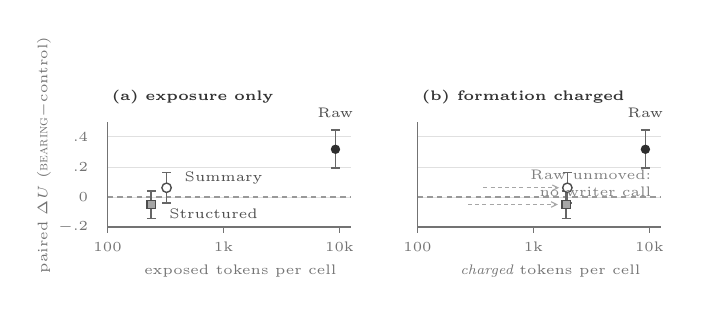
\begin{tikzpicture}[
  font=\scriptsize,
  ax/.style={draw=black!55, line width=0.4pt},
  gl/.style={draw=black!12, line width=0.3pt},
  zl/.style={draw=black!40, line width=0.4pt, dash pattern=on 2pt off 1.5pt},
  tk/.style={font=\tiny, text=black!55},
  hd/.style={font=\tiny\bfseries, text=black!80},
  lb/.style={font=\tiny, text=black!70},
  whisk/.style={draw=black!60, line width=0.6pt},
]
%% ---------- shared y axis, drawn once on the left ----------
\foreach \y/\l in {\frYTickMinusTwo/{$-$.2}, \frYTickZero/{0}, \frYTickTwo/{.2}, \frYTickFour/{.4}}
  \node[tk, left=1.5pt] at (-2pt,\y) {\l};
\node[tk, rotate=90, anchor=south] at (-17pt,26pt) {paired $\Delta U$ (\textsc{bearing}$-$control)};

%% ================= LEFT PANEL: exposure only =================
\begin{scope}
  \foreach \y in {\frYTickMinusTwo, \frYTickZero, \frYTickTwo, \frYTickFour}
    \draw[gl] (0,\y) -- (\frW,\y);
  \draw[zl] (0,\frZeroY) -- (\frW,\frZeroY);
  \draw[ax] (0,0) -- (0,\frH);
  \foreach \x/\l in {\frXTickTwo/{100}, \frXTickThree/{1k}, \frXTickFour/{10k}}{
    \draw[ax] (\x,0) -- (\x,-2pt);
    \node[tk, anchor=north] at (\x,-2pt) {\l};
  }
  \draw[ax] (0,0) -- (\frW,0);
  \node[tk, anchor=north] at (48pt,-10pt) {exposed tokens per cell};
  \node[hd, anchor=south west] at (-2pt,\frH+3pt) {(a) exposure only};
  % whiskers then markers, so the marker sits on top of its interval
  \draw[whisk] (\frRawXExp,\frRawYLo) -- (\frRawXExp,\frRawYHi);
  \draw[whisk] (\frSumXExp,\frSumYLo) -- (\frSumXExp,\frSumYHi);
  \draw[whisk] (\frStrXExp,\frStrYLo) -- (\frStrXExp,\frStrYHi);
  \foreach \x/\y in {\frRawXExp/\frRawYLo, \frRawXExp/\frRawYHi, \frSumXExp/\frSumYLo,
                     \frSumXExp/\frSumYHi, \frStrXExp/\frStrYLo, \frStrXExp/\frStrYHi}
    \draw[whisk] (\x-1.6pt,\y) -- (\x+1.6pt,\y);
  \fill[black!82] (\frRawXExp,\frRawY) circle (1.7pt);
  \draw[draw=black!70, fill=white, line width=0.5pt] (\frSumXExp,\frSumY) circle (1.7pt);
  \draw[draw=black!70, fill=black!35, line width=0.4pt]
    (\frStrXExp-1.5pt,\frStrY-1.5pt) rectangle (\frStrXExp+1.5pt,\frStrY+1.5pt);
  \node[lb, anchor=south] at (\frRawXExp,\frRawYHi+1pt) {Raw};
  \node[lb, anchor=west] at (\frSumXExp+3pt,\frSumY+3.5pt) {Summary};
  \node[lb, anchor=west] at (\frStrXExp+3pt,\frStrY-3.5pt) {Structured};
\end{scope}

%% ================= RIGHT PANEL: formation charged =================
\begin{scope}[xshift=112pt]
  \foreach \y in {\frYTickMinusTwo, \frYTickZero, \frYTickTwo, \frYTickFour}
    \draw[gl] (0,\y) -- (\frW,\y);
  \draw[zl] (0,\frZeroY) -- (\frW,\frZeroY);
  \draw[ax] (0,0) -- (0,\frH);
  \foreach \x/\l in {\frXTickTwo/{100}, \frXTickThree/{1k}, \frXTickFour/{10k}}{
    \draw[ax] (\x,0) -- (\x,-2pt);
    \node[tk, anchor=north] at (\x,-2pt) {\l};
  }
  \draw[ax] (0,0) -- (\frW,0);
  \node[tk, anchor=north] at (48pt,-10pt) {{\itshape charged} tokens per cell};
  \node[hd, anchor=south west] at (-2pt,\frH+3pt) {(b) formation charged};
  % the shift each model-written arm takes when its writer call is billed
  \draw[draw=black!35, line width=0.4pt, -{Straight Barb[length=2pt,width=2pt]},
        dash pattern=on 1.4pt off 1.2pt]
    (\frSumXExp+2.5pt,\frSumY) -- (\frSumXChg-3pt,\frSumY);
  \draw[draw=black!35, line width=0.4pt, -{Straight Barb[length=2pt,width=2pt]},
        dash pattern=on 1.4pt off 1.2pt]
    (\frStrXExp+2.5pt,\frStrY) -- (\frStrXChg-3pt,\frStrY);
  \draw[whisk] (\frRawXChg,\frRawYLo) -- (\frRawXChg,\frRawYHi);
  \draw[whisk] (\frSumXChg,\frSumYLo) -- (\frSumXChg,\frSumYHi);
  \draw[whisk] (\frStrXChg,\frStrYLo) -- (\frStrXChg,\frStrYHi);
  \foreach \x/\y in {\frRawXChg/\frRawYLo, \frRawXChg/\frRawYHi, \frSumXChg/\frSumYLo,
                     \frSumXChg/\frSumYHi, \frStrXChg/\frStrYLo, \frStrXChg/\frStrYHi}
    \draw[whisk] (\x-1.6pt,\y) -- (\x+1.6pt,\y);
  \fill[black!82] (\frRawXChg,\frRawY) circle (1.7pt);
  \draw[draw=black!70, fill=white, line width=0.5pt] (\frSumXChg,\frSumY) circle (1.7pt);
  \draw[draw=black!70, fill=black!35, line width=0.4pt]
    (\frStrXChg-1.5pt,\frStrY-1.5pt) rectangle (\frStrXChg+1.5pt,\frStrY+1.5pt);
  \node[lb, anchor=south] at (\frRawXChg,\frRawYHi+1pt) {Raw};
  \node[tk, anchor=north east, text=black!50, align=right] at (\frW,\frRawY-4pt)
    {Raw unmoved:\\no writer call};
\end{scope}
\end{tikzpicture}
\caption{Utility against cost for the same $\frMems$ memories on the same
$\frCells$ cells, under the two cost accountings, \emph{single-model
throughout}. Points are the paired within-memory effect; whiskers are $95\%$
bootstrap intervals over memories; the $x$ axis is logarithmic, so
\emph{efficiency is the slope from the origin}. \textbf{(a)} Counting only
the tokens the reader is shown, Summary sits $\frRatioExp\times$ above Raw
per exposed token. \textbf{(b)} Charging the writer's own call, amortized
over the $\frReuse$ cells that reuse each memory, moves the model-written
arms right by $\frFormSum$ and $\frFormStr$ tokens per cell and leaves Raw
exactly where it was, since it makes no extraction call --- so the ordering
\emph{depends on which cost is counted}. Neither panel licenses Summary as an
operating point: its interval spans zero in both ($\frSumLo$ to $\frSumHi$),
as does Structured's, and only Raw's excludes it. The figure establishes the
\emph{trade}, not a winner.}
\label{fig:frontier}
\end{figure}

\subsection{Representation changes downstream utility}
\label{sec:repr}
%%% Source: docs/REPRESENTATION_RESULT.md; results/repr_scaleup/cells.jsonl.
%%% Join key is (memory_unit_locator, future_task_id) -- memory_id is a
%%% per-representation content hash and matches zero rows across arms.
Repeating the measurement on the same experiences and tasks, changing only
how the experience is written down, separates the three representations. On
the 277 cells evaluated under all three, the paired \textsc{bearing}$-$control
effect is $+0.3174$ for Raw (95\% CI $[+0.19, +0.45]$), $+0.0613$ for Summary
($[-0.04, +0.16]$) and $-0.0498$ for Structured ($[-0.14, +0.04]$). Only Raw
excludes zero: at compression ratios of $0.063$ and $0.037$, rewriting the
experience removes the benefit, and the loss falls in \textsc{bearing}, where
there was an effect to lose. Against cost (Figure~\ref{fig:frontier}),
compression buys a smaller context, not a better return.



\subsection{Cost changes the apparent efficiency tradeoff}
\label{sec:cost}
%%% MOVED here beside the frontier figure, 2026-10-01. No number is typed:
%%% \frRatioExp, \frRatioChg, \frReuse, \frFormSum and \frFormStr are generated
%%% macros, and audit_claims.py pins BOTH ratios (5.52 uncharged, 1.10 charged)
%%% and FAILS the build on the withdrawn "roughly 5x" wording -- charged,
%%% Summary is INDISTINGUISHABLE from Raw, not five times worse, and the
%%% understatement was the defect the audit was extended to catch.
Utility per exposed token is not the same quantity as utility per token the
system had to pay for. Counting only what the reader is shown, Summary sits
$\frRatioExp\times$ above Raw and compression looks like the efficient
choice. Charging each representation for writing itself --- amortized over
the $\frReuse$ cells that reuse one memory --- moves the two model-written
arms right by $\frFormSum$ and $\frFormStr$ tokens per cell and leaves Raw
exactly where it was, since Raw makes no extraction call
(Figure~\ref{fig:frontier}). Raw's charged margin over Summary is then
$\frRatioChg\times$: compression's apparent advantage does not reverse into a
large one, it \emph{disappears}. Which representation looks efficient
therefore depends on which cost is counted, and neither accounting licenses
Summary as an operating point --- its interval spans zero in both ($\frSumLo$
to $\frSumHi$).

\subsection{Cross-benchmark boundary}
\label{sec:crossbench}
%%% MOVED out of Limitations, 2026-10-01: this is a RESULT about the SCOPE of
%%% the representation ordering, reported as a bound rather than a caveat.
%%% Every value is the same figdata.tex macro as before; make_figures.py still
%%% fails the build if any SciCode or SWE-bench interval stops crossing zero,
%%% and audit_claims.py fails if the manuscript ever implies all three
%%% benchmarks show one effect.
The one quantity all three benchmarks define identically is the paired
representation contrast, and it separates from zero on LongMemEval-V2 alone
(Table~\ref{tab:crossbench}). On SciCode and on SWE-bench Verified every
interval crosses zero, and doubling the SciCode cell count separated none of
them. We therefore state a boundary rather than a second confirmation:
\emph{LongMemEval-V2's Raw-dominant ordering does not generalize as an
established ordering to either benchmark.} The two secondary runs bound the
primary result; the three benchmarks are not evidence of one common effect.

%%% ============ TABLE: cross-benchmark paired representation contrasts =====
%%% WAS A FOREST FIGURE. Converted to a table 2026-10-01: six intervals in a
%%% ruled plot cost ~62pt of float height that the 8-page body could not pay
%%% for once the reader-generalization figure was added, and the plot's only
%%% visual claim -- which intervals cross zero -- is read as fast from the
%%% printed endpoints. EVERY VALUE IS THE SAME MACRO from figdata.tex; no
%%% number changed in the conversion, and make_figures.py still FAILS the
%%% build if any SciCode or SWE-bench interval stops crossing zero, if
%%% either ORDERING_VERDICT changes, if the defect-21 correction is reverted,
%%% or if SWE-bench ever acquires a WITHOUT-arm floor (0 by construction).
\begin{table}[t]
\centering\small
\setlength{\tabcolsep}{4pt}
\caption{The paired representation contrast, the one quantity these
benchmarks define identically: $\Delta U$ under one representation minus
$\Delta U$ under Raw, \emph{per cell} on the same memory and task,
task-clustered 95\% intervals. Only LongMemEval-V2 separates from zero, in
both rows. \textbf{Every SciCode and every SWE-bench interval crosses zero},
so the differing point-estimate ordering is not an established reversal, and
doubling the SciCode cell count did not separate any contrast. We compare
contrasts rather than per-representation $\Delta U$ because each benchmark
carries its own nondeterminism --- the no-memory arm, where the question is
identical across representations, still disagrees on
$\xbFloorLmK/\xbFloorLmN{=}\xbFloorLm$ of LongMemEval-V2 cells and
$\xbFloorScK/\xbFloorScN{=}\xbFloorSc$ on SciCode --- and a paired contrast
differences that term out.}
\label{tab:crossbench}
\begin{tabular}{@{}llrrr@{}}
\toprule
contrast & benchmark & $n$ & mean & 95\% CI \\
\midrule
Summary $-$ Raw
 & LongMemEval-V2 & \xbSRLmN & \xbSRLmM & [\xbSRLmLo, \xbSRLmHi] \\
 & SciCode        & \xbSRScN & \xbSRScM & [\xbSRScLo, \xbSRScHi] \\
 & SWE-bench      & \xbSRSwN & \xbSRSwM & [\xbSRSwLo, \xbSRSwHi] \\
\midrule
Structured $-$ Raw
 & LongMemEval-V2 & \xbTRLmN & \xbTRLmM & [\xbTRLmLo, \xbTRLmHi] \\
 & SciCode        & \xbTRScN & \xbTRScM & [\xbTRScLo, \xbTRScHi] \\
 & SWE-bench      & \xbTRSwN & \xbTRSwM & [\xbTRSwLo, \xbTRSwHi] \\
\bottomrule
\end{tabular}
\end{table}

%%% ============ FIGURE 6: READER TRANSFER (CANONICAL, SESSION-MATCHED) ====
%%% REDESIGNED. The previous version drew \rgRawDiff -- the SUPERSEDED
%%% cross-session contrast (+0.1268, arms 11 hours apart) -- while the prose
%%% beside it quoted the canonical session-matched +0.0982. A reader
%%% comparing the marker to the paragraph found two different numbers for
%%% one claim, and no check could fail. This figure draws ONLY the canonical
%%% arm, and scripts/make_figures.py::reader_session_matched() fails the
%%% build if the two estimates ever become indistinguishable, if the arms
%%% stop sharing one session, or if the verdict changes.
%%%
%%% WHY ONE INTERVAL AND NOT TWO. The two readers' OWN 95% intervals overlap
%%% by 0.0689 (gpt-oss tops at +0.3025, Gemma starts at +0.2336). Drawing
%%% both would invite "the intervals overlap, so no difference" -- which is
%%% FALSE: the cells are paired and the paired interval excludes zero. The
%%% generator asserts that overlap, so if the marginals ever separate the
%%% rationale stated in this caption must be re-argued rather than silently
%%% outliving its reason.
%%%
%%% PANEL B is the matched per-cell cross-tabulation, which answers the
%%% question Panel A cannot: not "is the mean higher" but "is it the same
%%% cells". It is reported on cells that CAN move -- 170 of 275 are zero
%%% under both readers, and counting those as agreement would report ~82%
%%% agreement for cells that could not have disagreed.
\begin{figure}[t]
\centering
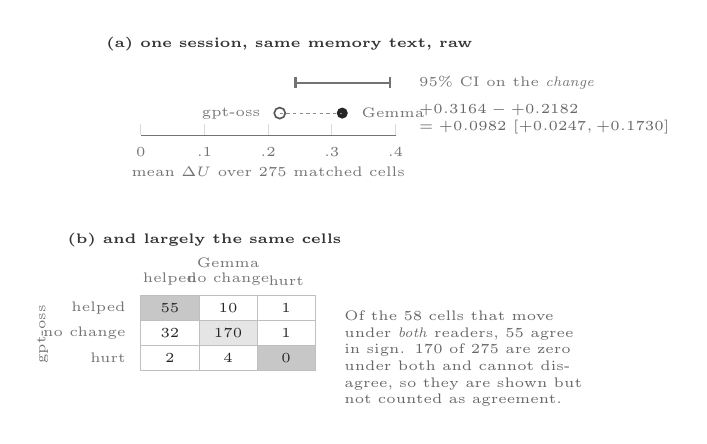
\begin{tikzpicture}[
  font=\scriptsize,
  ax/.style={draw=black!55, line width=0.4pt},
  gl/.style={draw=black!15, line width=0.3pt},
  tk/.style={font=\tiny, text=black!55},
  hd/.style={font=\tiny\bfseries, text=black!80},
  lg/.style={font=\tiny, text=black!60},
  wh/.style={line width=0.8pt},
]
%% ================= PANEL A: the canonical reader contrast =================
\node[hd, anchor=south west] at (-16pt,23pt)
  {(a) one session, same memory text, \textsc{raw}};
\foreach \x/\l in {\smTickZero/0, \smTickOne/{.1}, \smTickTwo/{.2},
                   \smTickThree/{.3}, \smTickFour/{.4}}{
  \draw[gl] (\x,-4pt) -- (\x,0pt);
  \node[tk, anchor=north] at (\x,-5pt) {\l};
}
\draw[ax] (0pt,-4pt) -- (\smW,-4pt);
\node[tk, anchor=north] at (46pt,-12pt) {mean $\Delta U$ over \rgSmCells\ matched cells};
%% the paired interval, anchored at the gpt-oss point. Legitimate because the
%% mean of the per-cell differences IS the gap between the means on a paired
%% set; make_figures.py asserts that identity exactly.
\draw[wh, black!55] (\smXCiLo,15pt) -- (\smXCiHi,15pt);
\draw[wh, black!55] (\smXCiLo,13pt) -- (\smXCiLo,17pt);
\draw[wh, black!55] (\smXCiHi,13pt) -- (\smXCiHi,17pt);
\node[tk, anchor=west] at (\smW+5pt,15pt)
  {95\% CI on the \emph{change}};
%% the two reader points, on one row so the gap IS the effect
\draw[draw=black!65, fill=white, line width=0.6pt] (\smXOss,4pt) circle (2.0pt);
\fill[black!85] (\smXGem,4pt) circle (2.0pt);
\draw[draw=black!45, line width=0.4pt, dash pattern=on 1.2pt off 1.2pt]
  (\smXOss,4pt) -- (\smXGem,4pt);
\node[tk, anchor=east] at (\smXOss-3.5pt,4pt) {gpt-oss};
\node[tk, anchor=west] at (\smXGem+3.5pt,4pt) {Gemma};
\node[lg, anchor=west] at (\smW+5pt,5pt)
  {$\rgSmGem-\rgSmOss$};
\node[lg, anchor=west] at (\smW+5pt,-1pt)
  {$=\rgSmDiff$ $[\rgSmLo,\rgSmHi]$};
%% ================= PANEL B: is it the SAME cells? =========================
\begin{scope}[yshift=-62pt]
\node[hd, anchor=south west] at (-30pt,14pt) {(b) and largely the same cells};
\def\cwd{21pt}\def\cht{9pt}
%% column headers = Gemma's verdict, row headers = gpt-oss's
\foreach \c/\lab in {0/helped, 1/no change, 2/hurt}
  \node[tk, anchor=south] at ({\c*\cwd+0.5*\cwd},{0.2pt}) {\lab};
\node[tk, anchor=south] at (31.5pt,6.5pt) {Gemma};
\foreach \r/\lab in {0/helped, 1/{no change}, 2/hurt}
  \node[tk, anchor=east] at (-2pt,{-\r*\cht-0.5*\cht}) {\lab};
\node[tk, rotate=90, anchor=south] at (-30pt,-14pt) {gpt-oss};
%% the nine counts. Diagonal cells are shaded: those are the agreements.
\foreach \r/\c/\v/\sh in {%
   0/0/\smCPosPos/22, 0/1/\smCPosZero/0, 0/2/\smCPosNeg/0,
   1/0/\smCZeroPos/0, 1/1/\smCZeroZero/10, 1/2/\smCZeroNeg/0,
   2/0/\smCNegPos/0, 2/1/\smCNegZero/0, 2/2/\smCNegNeg/22}{
  \fill[black!\sh] ({\c*\cwd},{-\r*\cht-\cht}) rectangle ++(\cwd,\cht);
  \draw[draw=black!25, line width=0.3pt]
    ({\c*\cwd},{-\r*\cht-\cht}) rectangle ++(\cwd,\cht);
  \node[tk, text=black!85] at ({\c*\cwd+0.5*\cwd},{-\r*\cht-0.5*\cht}) {\v};
}
\node[lg, anchor=north west, align=left, text width=86pt] at (70pt,-2pt)
  {Of the \smBoth\ cells that move under \emph{both} readers,
   \smAgree\ agree in sign. \smZeroBoth\ of \rgSmCells\ are zero under both
   and cannot disagree, so they are shown but not counted as agreement.};
\end{scope}
\end{tikzpicture}
\caption{\textbf{The Raw memory effect survives a second reader.}
\textbf{(a)} Both readers re-executed \emph{in one session}, with the memory
text, the filler pool and the whole rendered request hash-identical on
$\smIdentK/\smIdentN$ joinable rows, so only the reader differs --- this is
the measurement we quote. Mean $\Delta U$ rises from $\rgSmOss$ to
$\rgSmGem$ over $\rgSmCells$ matched cells on $\rgSmTasks$ tasks
($\rgSmN$ replicate rows; the three counts are different units and are not
interchangeable). The single interval is the \emph{paired}
one, $\rgSmDiff$ $[\rgSmLo, \rgSmHi]$, anchored at the gpt-oss point so it
clears that point exactly when the change excludes zero; the readers' own
intervals overlap, and plotting those would invite a ``no difference''
reading the paired design rules out. \textbf{(b)} The same
cells, cross-tabulated. The readers agree in sign on $\smAgree$ of the
$\smBoth$ cells where both move; the $\smZeroBoth$ cells that are zero under
both are shown but excluded from that rate, since a cell that cannot move
cannot disagree. Gemma also helps on $\smCZeroPos$ cells gpt-oss left
unchanged, which is why its mean is higher.}
\label{fig:readertransfer}
\end{figure}

\subsection{Memory utility survives a change of reader}
\label{sec:readertransfer}
%%% Source: docs/READER_TRANSFER_RESULT.md; artifacts
%%% results/ledgers/gemma_reader/reader_transfer_analysis.json and the slim
%%% row slice results/ledgers/repro/gemma_reader/transfer_cells_slim.jsonl.
%%% Pre-registered in docs/READER_TRANSFER_PRECOMMITMENT.md BEFORE any
%%% design-cell call was issued: no transfer, same ordering with different
%%% magnitude, and a different representation preference were all committed
%%% as valid outcomes, so this is a test rather than a confirmation.
%%% RAW MAY BE STATED AS A POSITIVE FINDING -- its interval excludes zero.
%%% SUMMARY AND STRUCTURED SPAN ZERO AND MUST NOT BE. make_figures.py fails
%%% the build if either half of that inverts; verified by planting both.
%%% Every number here is a macro from figdata.tex; none is typed.
Is the representation result an artifact of one model reading memories the
same model wrote? It is not. We re-executed the representation sub-universe
with a second, unrelated reader on the \emph{same memory text}: the memory
file, prompt, filler pool, every rendered request and each cell's target
position were hash-asserted against the first run at call time, and the text
re-verified $\rgRows/\rgRows$ byte-identical.

\textbf{The effect transfers, and on Raw it is larger}
(Figure~\ref{fig:readertransfer}). With both readers run \emph{in one
session} --- the measurement we quote, this endpoint not being deterministic
across them --- the second reader's $\Delta U$ exceeds the first's on Raw by
$\rgSmDiff$ $[\rgSmLo$, $\rgSmHi]$, which excludes zero
($\rgSmCells$ cells, $\rgSmTasks$ tasks). The
within-memory bearing$-$control contrast rises from $\rgBmcRawOss$
$[\rgBmcRawOssLo$, $\rgBmcRawOssHi]$ to $\rgBmcRawGem$ $[\rgBmcRawGemLo$,
$\rgBmcRawGemHi]$, and the Raw-dominant ordering holds. Summary $\rgSumDiff$
$[\rgSumLo$, $\rgSumHi]$ and Structured $\rgStrDiff$ $[\rgStrLo$, $\rgStrHi]$
span zero, but with only $\rgSumNNz$ and $\rgStrNNz$ cells non-zero under
either reader those are \emph{underpowered}, not \emph{no difference}. Part
of the gain is a weaker reader rather than a better memory --- the no-memory
arm moves $\rgWithoutDelta$ --- but it does not divide cleanly. A
first execution a day apart returned $\rgRawDiff$ $[\rgRawLo$, $\rgRawHi]$,
inside the session-matched interval; re-run together, that arm splits
$-0.0327$ by session against $-0.0364$ by reader, halving the apparent
reader share.

\paragraph{The readers agree on ordering and direction, not cell by cell.}
Over all matched Raw cells the readers' per-cell $\Delta U$ correlate at
$r{=}\rgRawRAll$, but $\rgRawZeroBoth$ of $\rgRawN$ cells are exactly zero
under both, and a cell that could not move counts there as perfect agreement.
Restricted to the $\rgRawNNz$ non-zero under either, $r$ falls to
$\rgRawRNz$ --- the honest figure, given beside the inflated one
($\rgSumRNz$, $\rgStrRNz$ on Summary and Structured). Where both move they move
together: signs agree on $\rgRawSignK$ of $\rgRawSignN$ Raw cells, labels on
$\rgRawLabK$ of $\rgRawLabN$. The zeros are structural (Section~\ref{sec:scarcity}), but a reviewer asking
whether it is \emph{the same} memories that help does not yet have a clean
yes. Cost is not pooled
across models: the second reports no reasoning-token counts, so
Figure~\ref{fig:frontier}'s axis is single-model throughout. A pre-registered writer
$\times$ reader factorial, all four arms in one session, returns a null:
every one of its eight contrasts spans zero --- writer, reader, same-family
and interaction, on Summary ($n{=}274$) and Structured ($n{=}268$). The
intervals are informative rather than underpowered, excluding writer and
same-family effects beyond $0.0380$ against the $\rgSmDiff$ reader effect
this apparatus does detect; but Raw has no writer and is not in the factorial, and
two checkpoints are a $2\times2$, not a population.
\textsc{bearing} contains 2 negative cells against 50 positive, but we
report no harmful-memory rate: the design screened \emph{for} bearing, so a
harm rate here would be a selected-subgroup estimate, and the unscreened
stratum's $26/872$ is no natural base rate either, the pairing being ours.


\subsection{What the instrument did not find}
\label{sec:r0}
%%% Source: docs/THE_HONEST_HEADLINE.md and
%%% docs/ADDITIVE_NULL_AND_DECOMPOSITION.md; re-derived by the coordinating
%%% author from results/deltau_screened/cells.jsonl. This subsection LEADS the
%%% results deliberately: it reports a negative on the hypothesis the study was
%%% built around, and burying it would misrepresent what the measurement found.
%%%
%%% TABLE 1 (sign reversal by stratum) WAS REMOVED HERE, 2026-09-30. It plotted
%%% the same three strata, rates, Wilson intervals and denominators as
%%% Figure~\ref{fig:bearing}(b) -- whose values are GENERATED into figdata.tex
%%% by scripts/make_figures.py, whereas the table's were typed. Two displays of
%%% a DEMOTED metric, one of them hand-entered, is the wrong allocation of an
%%% eight-page budget. Removing it paid for the Discussion rewrite. The numbers
%%% survive in the figure and in scripts/audit_claims.py, which re-derives every
%%% one of them; nothing became unciteable.
%%%
%%% THE SECOND NEGATIVE (the additive null) IS NEW HERE. Only its SIGN is
%%% quoted, never its magnitude: two implementations agree the excess is
%%% negative in all three strata but disagree on how negative (Master Agent
%%% -0.3854/-0.5830/-0.7133 vs Sub-agent K -0.2286/-0.6857/-0.7167; neither is
%%% audited as canonical). The sign is what the claim turns on.
We set out to measure a rate of sign reversal: the frequency with which one
memory helps one future task and harms another. On cells where the memory
demonstrably bears on the task, that rate is zero (Figure~\ref{fig:bearing}b).
Two features of it matter more than the zero. It is \emph{bounded}: with 35
flip-eligible memories over 21 source episodes the Wilson upper bound is
$0.0989$, so the rate is below about ten percent rather than merely
unobserved. And the reversals that do occur concentrate in the unscreened
stratum, where memories are paired with tasks they have no relationship to
($17/60$, against $0/35$ and $1/35$; the \textsc{bearing} and \textsc{random}
intervals are disjoint, Fisher one-sided $p = 1.5\times10^{-4}$). A sign
reversal between a memory and an unrelated task is weak evidence that utility
is task-conditional and strong evidence that both executions sat near the
reader's failure floor. A study pairing indiscriminately will measure a reversal rate near $0.28$,
this run's own \textsc{random} stratum, substantially an artifact of the
pairing. Our two earlier unscreened arms, paired by a different rule, reverse
on $8/60$ memories ($0.133$) each, so the inflation is a property of the
pairing rule and not a constant.

\paragraph{Fewer reversals than additivity alone predicts.}
The pre-registered standard (Section~\ref{sec:metrics}) asked for the excess
of the observed reversal rate over a fitted additive model with the
interaction removed. Fitting $\mu + a_m + b_t$ and simulating from it, that
excess is \emph{negative in all three strata}; two implementations disagree
on the magnitude and agree on the sign, so we quote only the sign. The
standard is not merely unmet but met in the wrong direction, and its other
leg is not estimable here.

\paragraph{What this leaves.}
A single scalar $\mathrm{Value}(m)$ remains inadequate, but for a different
reason than we hypothesised: not because a memory's sign varies with the
task, but because its value is \emph{sparse}, concentrated on the rare tasks
it bears on and averaged away over the majority on which it is inert.

\section{Reproducibility}
Every number here is registered in a results ledger naming the artifact that
produced it and the date it was measured, and every figure's values are
recomputed from those artifacts by a generator that fails the build when one
stops supporting the caption written over it --- each guard verified by
planting its defect, which is how the scoring error in
Section~\ref{sec:setup} and one vacuous check of our own were found. The
released dataset is one row per evaluated cell over memory $\times$ task
$\times$ representation $\times$ replicate, carrying utility, full output
text and per-family cost. Four properties are enforced by a validator rather
than documented: the retention of full text rather than a digest, so a cell
can be re-scored under a corrected verifier; continuous rewards; reader and
writer cluster never null; and content-hash identifiers the validator
recomputes. \textbf{Text retention holds for 5{,}641 of the 5{,}924 released
rows, and the 283 exceptions have two different causes, marked by two
different sentinels.} On 154 SciCode rows the reader output was never
persisted by the run that produced it --- the rewards are valid, the text is
gone, and it cannot be regenerated, because this endpoint is deterministic
within a session and not across one; on 127 SWE-bench rows the text exists
and we may not redistribute it. A persistence gap and a licence withholding
are not the same fact and the release does not spell them the same way.

\section{Limitations}
\label{sec:limitations}
%%% Sources: docs/MASTER_TODO.md P1-116/127/128/129, docs/LEAKAGE_AUDIT.md,
%%% docs/MEMORY_REPRESENTATIONS.md Sec. 5 and 7, docs/BENCHMARK_DECISIONS.md,
%%% docs/ANALYSIS_PREREGISTRATION.md Sec. 5.

\paragraph{The matrix is constructed, not harvested.}
The memories are naturally occurring spans of real past trajectories
(Section~\ref{sec:setup}), but the \emph{pairing} to future tasks is ours: we
checked for natural (memory, task) co-occurrences, found none usable, and
construct the grid by a deterministic seeded rule fixed before measurement. Every rate is therefore \textbf{over a defined task set}, never
an unqualified natural base rate: the task set is part of the estimand.

\paragraph{Leakage rates are lower bounds, from a bug in the official scorer.}
Our detector reuses the benchmark's own phrase matcher, whose normalizer
strips punctuation without inserting a space: a gold phrase abutting a quote
or an equals sign is glued to its neighbour and the match fails. Such leaks
are \emph{missed}, and punctuation is constant in accessibility trees, so
every leakage rate we report is a lower bound. It is pinned as an
expected-failure control, so a future upstream fix fails loudly. The 156 LLM-judged questions are
\emph{undecidable} without an inference call and recorded as such rather than
clean; 69 multiple-choice questions with one-to-five-character gold answers
are structurally un-auditable and never folded into a pooled rate.

\paragraph{Our reader is deterministic within a session, not across sessions.}
Every floor we report is a \emph{within-session} floor: $F_{\mathrm{exec}}$
replicates are issued seconds apart in one run and agree on 1{,}157 of 1{,}157
cells, and $F_{\mathrm{judge}}$ is six re-scorings in one run agreeing on 240
of 240. Both are correct at that scope and neither licenses cross-session
reproducibility --- re-issuing byte-identical \emph{no-memory} requests a day
later returned different text in 554 of 1{,}124 cases and moved the no-memory
baseline by $-0.030$, the same order as the effects we measure, while a second
reader drifted $0$ of $1{,}124$, making this a property of the model rather
than the serving stack. We therefore compare arms executed in one session, under an amendment
pre-registered before any contrast was computed, and re-ran both readers
together where a comparison already spanned sessions --- which inflated that
decomposition though not the effect (Section~\ref{sec:readertransfer}). We
have no cross-session floor for any arm and presume it non-zero here. A zero
floor is also a fact about the apparatus before it is one about the subject:
our judge returned byte-identical text, free-text reason included, on all 288
floor re-scorings, so $F_{\mathrm{judge}}{=}0$ measures greedy decoding rather
than an unambiguous rubric --- and SciCode's equivalent control disagrees on 5
of 135 cells \emph{within} one session, so determinism may not be assumed of a
new benchmark either.

\paragraph{Two axes we cannot yet rely on.}
We intended semantic type as a second axis, but in our representation pilot
the two labelling passes agreed on 3 of 8 segments at \textbf{Cohen's
$\kappa = 0.000$}: the structured writer's native pass called every segment
\texttt{episodic}, a degenerate marginal whose agreement carries no
information beyond the classifier's prior, so we report no semantic-type
breakdown. Separately, exactly one deterministically scorable \emph{errors-gotchas}
question exists benchmark-wide, accounting alone for 865 of 6,920 web cells,
so any per-stratum result there is a single-question result.

\paragraph{One cluster, one domain --- and pilot-scale representation
evidence.}
%%% UPDATED. An earlier version of this paragraph said the results come from
%%% a single reader and that we cannot tell whether the effect is a property
%%% of memory or of that reader. Section 8.8 now answers the reader half
%%% directly, so leaving the sentence would understate what was measured; the
%%% cluster and domain halves are unchanged and still hold.
Every cell runs on a single serving cluster, since pooling across serving
configurations would confound; the failover configuration is a separate arm,
not extra data. The reader half of this limitation is now answered --- a second reader on
the identical memories reproduces the ordering and the effect
(Section~\ref{sec:readertransfer}) --- and the \emph{writer} half returns a
null across a pre-registered $2\times2$
(Section~\ref{sec:readertransfer}). Two limits on that null are structural:
Raw, the representation that wins, is written by no model and so has no
writer axis to vary, and two checkpoints on one cluster establish nothing
about model families. Our cross-domain evidence remains a case study rather
than a second main table (Table~\ref{tab:crossbench}). The structured writer
failed on $3$ of $60$ segments, all three by exhausting the token budget
mid-value rather than malforming output, and $0$ of the $57$ writes that
finished; an 8-segment pilot had put that at $0$ of $8$ and could not have
seen it, never having met the cap. Our faithfulness measures are a screen, not a guarantee: a low score is
strong evidence of a problem, a high score weak evidence of its absence, and
they are blind to recombination, omission, unsupported inference and prose
negation. Two exclusions are stated
rather than silently taken: 17 of the 295 deterministically scored questions
have no memory unit carrying their gold answer, so their cells can only yield
$\Delta U \le 0$; and 23 of 1,889 units (1.2\%) are their entire trajectory.


\section*{Use of AI-Assisted Technologies}
%%% REQUIRED by AAMAS 2027 where AI contributed to hypotheses or experimental
%%% design; the stronger clause applies here because AI shaped DESIGN, not
%%% only code and polishing. Source: docs/AI_ASSISTANCE_DISCLOSURE.md, which
%%% quotes the verified policy text. Prompts go to supplementary material,
%%% which the policy permits.
This work used AI coding and research assistants (Claude Opus~5 via Claude
Code, 2026) under human direction, beyond text polishing: they implemented the
measurement harness, benchmark adapters, cell construction and analysis code,
executed the inference campaigns, and proposed elements of the experimental
design --- including the discriminative screening criterion and the
stratified bearing/matched-control/random design. We therefore disclose under
the stronger clause of the policy. Every quantitative claim was re-derived
from the row-level artifact by a verification pass independent of the agent
that produced it, and every citation was verified against a fetched primary
source. Prompts and the full defect register are in the supplementary
material.

\section{Discussion}
\label{sec:discussion}
%%% Sources: docs/THE_HONEST_HEADLINE.md (the reframing this section states),
%%% docs/ADDITIVE_NULL_AND_DECOMPOSITION.md (both negatives, with the excess's
%%% SIGN -- not its magnitude, which two implementations disagree on),
%%% docs/PROJECT_GOAL.md (the kill criterion, and why it did NOT fire).
%%% BINDING: no clause here may imply a sign change evidences interaction, and
%%% no variance share may be quoted -- it is not estimable on this design.
We propose no retention policy, gate, or memory system, and note that a
learned gate over these measurements may be a domain transfer of a known
result~\cite{when2tool}; our argument concerns the quantity such a system
needs. The component we
built the study around did not survive (Section~\ref{sec:r0}): clean per-cell
utilities and a variance decomposition are in tension, because a reader with
no execution noise leaves no residual scale to identify components against.
Sparsity, which replaces it, cuts three ways. On measurement, pairing
indiscriminately puts most cells where neither arm can succeed, reporting a
null indistinguishable from an absence. On retrieval
(Figure~\ref{fig:similarity}), what located the effect asks
what a memory \emph{contains} rather than what it resembles --- but it asks
using the gold answer, so it is an instrument and not a method. The honest
statement of the gap is that a deployable retriever would have to approximate,
without ground truth, a quantity that generic similarity currently tracks
poorly. And since one
experience written three ways does not carry the same benefit, a memory's
value belongs to the experience together with how it was written --- a
pairing that survives a second reader of the same bytes, and a writer
$\times$ reader factorial in which no contrast separates from zero
(Section~\ref{sec:readertransfer}), so it is evidence about the experience
rather than about one model --- though Raw, which wins, has no writer to
vary. Taken together: a global memory score is insufficient for a
task-specific keep-or-drop decision, because utility is sparse over future
tasks, concentrated on the few a memory bears on, and moved by how the
experience was written down and what its formation cost.


\balance
\bibliographystyle{ACM-Reference-Format}
\bibliography{p1refs}

\end{document}
